\providecommand{\lukufilter}[2]{#2} % ylikirjoitetaan kaanna_luku.sh -skriptistä.
\newcommand{\osa}[1]{\chapter{#1}} % osa
\newcommand{\nosa}[1]{\chapter*{#1} \addcontentsline{toc}{chapter}{#1}} %numeroimaton osa
\newcommand{\luku}[2]{\section{#2} \lukufilter{#1}{\input{maa1/TEORIA_#1} \input{maa1/TEHT_#1}}} % luku
\newcommand{\nluku}[2]{\section*{#2} \addcontentsline{toc}{section}{#2} \lukufilter{#1}{\input{maa1/#1}}} % numeroimaton luku
\newcommand{\vast}{\section*{Vastaukset} \addcontentsline{toc}{section}{Vastaukset} \begin{vastaussivu} \begin{Vastaus}{1}
		\alakohdat{
			§ $-16-(-8)=-16+8=-8$
			§ $\frac{8}{5} + \frac{2}{5}=\frac{10}{5} = 2$
			§ $\frac{2}{5} \cdot \frac{2}{3}=\frac{4}{15}$
			§ $-8x^2+x$
			§ $\frac{b}{a^2}$
		}
	
\end{Vastaus}
\begin{Vastaus}{2}
		\alakohdat{
			§ $20$, sillä $1\,\text{l}=1\,\text{dm}^3$
			§ $20\,\text{dm}^3=20\cdot(\text{dm})^3=20\cdot\text{d}^3\cdot\text{m}^3=20\cdot (\frac{1}{10})^3\,\text{m}^3=20\cdot\frac{1}{1\,000}\, \text{m}^3=\frac{20}{1\,000}\,\text{m}^3=\frac{2}{100}\,\text{m}^3=0,02\,\text{m}^3$
		}
	
\end{Vastaus}
\begin{Vastaus}{3}
		\alakohdat{
			§ $x=-\frac{11}{4}$
			§ $x=-3$ tai $x=3$
			§ $x=-\frac{1}{\sqrt[3]{3}}$
		}
	
\end{Vastaus}
\begin{Vastaus}{4}
		\alakohdat{
			§ $(-3)^2+3\cdot(-3)=0$
 	%		§ \begin{kuvaajapohja}{0.7}{-4}{4}{-4}{4
%		\kuvaaja{2x-8}{\qquad $g(x)=2x-8$}{black}
 %			      \end{kuvaajapohja}}
			§ $x=4$
		}
	
\end{Vastaus}
\begin{Vastaus}{5}
		\alakohdat{
		§ Aika kaksinkertaistuu.
		§ Aika puolittuu. %RATKAISUT
		}
	
\end{Vastaus}
\begin{Vastaus}{6}
		\alakohdat{
			§ Alennettu hinta on $25,95\,€-25,95\cdot0,15=25,95\,€\cdot(1-0,15)=25,95\,€\cdot0,75=22,06\,€\approx 22,05$ euroa
			§ Merkataan tuotteen alkuperäistä hintaa (esimerkiksi) $x$:llä, jolloin saadaan yhtälö $x\cdot 0,75=21,25\,€$. Tästä saadaan ratkaistua jakolaskulla alkuperäiseksi hinnaksi $x=\frac{21,25\,€}{0,75}=25,00\,€$
		}
	
\end{Vastaus}
\begin{Vastaus}{7}
	\alakohdatm{
	§ $37\,616,003$
	§ $-67\,360\,008$
	}
	
\end{Vastaus}
\begin{Vastaus}{8}
	\alakohdat{
		§ Kukaan ei ole itsensä sisar, joten relaatio ei ole refleksiivinen.
		§ Sisaruus on aina molemminpuolista (jos $a$ on $b$:n sisar, niin myös $b$ on $a$:n sisar), joten relaatio on symmetrinen.
		§ Jokainen mielivaltaisen henkilön sisar on myös muiden kyseisen henkilön sisarten sisar (sisaruus ''välittyy eteenpäin''), joten relaatio on transitiivinen.
	}
	
\end{Vastaus}
\begin{Vastaus}{9}
	\alakohdat{
	§ refleksiivinen ja transitiivinen
	§ transitiivinen
	§ ei mikään vaihtoehdoista
	§ symmetrinen (ei transitiivinen, koska oma työkaveri voi olla töissä lisäksi jossain muualla)
	}
	
\end{Vastaus}
\begin{Vastaus}{10}
	Relaatio on symmetrinen, symmetrinen ja transitiivinen.
	
\end{Vastaus}
\begin{Vastaus}{11}
    	\alakohdatm{
        § epätosi
        § epätosi
        § tosi
        § tosi
        § tosi
        }
    
\end{Vastaus}
\begin{Vastaus}{12}
    	Pisteeseen
        \alakohdat{
            § $-2+(-3)=-5$
            § $-2+6+(-2)=2$
            § $-2+2+(-6)=-6$
        }
    
\end{Vastaus}
\begin{Vastaus}{13}
        \alakohdat{
            § $17-5=12$
            § $5+6=11$
            § $-10+(-2)=-12$
            § $-20-(-3)=-17$
        }
    
\end{Vastaus}
\begin{Vastaus}{14}
    \alakohdatm{
        § $h$
        § $-h$
        § $0$
        § $0$
    }
	
\end{Vastaus}
\begin{Vastaus}{15}
    \alakohdatm{
        § $-5$
        § $12$
        § $-3$
        § $3$
        § $0$
    }
	
\end{Vastaus}
\begin{Vastaus}{16}
    \alakohdatm{
        § $-36$
        § $-49$
        § $40$
        § $-64$
        § $-40$
        § $-80$
    }
	
\end{Vastaus}
\begin{Vastaus}{17}
	\alakohdat{
		§ $5:(-15)=-\frac{1}{3}$
		§ $-(2\cdot8)=-16$
		§ $\frac{-(-2)}{x-y}=\frac{2}{x-y}$
	}
	
\end{Vastaus}
\begin{Vastaus}{18}
		\alakohdat{
		§ Sivulle $92$. Luku saadaan laskutoimituksesta $47+3\cdot 15$.
		§ $490$ riviä. Luku saadaan laskutoimituksesta $2\,450:5$. (Kirjoitettujen rivien laskeminen on muuten oikeasti \textit{erittäin} huono tapa seurata työn tehokkuutta.)
		§ $121$ sivua
		§ $58$ sivua
		§ $60$ sivua
		§ $17$ pistettä. Luku saadaan laskutoimituksesta $8+(20-11)$. (Sulkeet selkeyden vuoksi.)
		§ $8$ minuuttia. Vastaukseen päädytään laskemalla ensin kulunut aika minuuteissa $32-15$ ja vähentämällä tämä $25$ minuutista: $25-(32-15)$. (Tai $25-7$, kun $32-15$ on jo laskettu.)
		}
	
\end{Vastaus}
\begin{Vastaus}{19}
	\alakohdat{
	§ Aseta herätysajaksi $9.30$. Jos puhelimesi näyttää Ruotsin aikaa, ongelmaa ei ole. Jos puhelimesi on Suomen ajassa, puhelimesi herättää sinut tuntia aiemmin, mutta tällöin et ainakaan myöhästy. Sitä aikaisemmaksi on turha herätystä asettaa -- se vie vain unelta tunteja.
	§ Herätysajaksi kannattaa asettaa $7.30$. Jos puhelimesi näyttää Suomen aikaa, Moskovassa on kello tällöin juuri sopivasti $9.30$. Jos puhelimesi näyttää Moskovan aikaa (tai välissä olevaa tunnin Suomesta edellä olevaa aikaa), herätys on aikaisintaan kello $7.30$, jolloin olet kuitenkin ajoissa.
	}
	
\end{Vastaus}
\begin{Vastaus}{20}
$(49-33):4=16:4=4$ eli $4$ pistettä
	
\end{Vastaus}
\begin{Vastaus}{21}
	\alakohdatm{
	§ $36$ minuuttia
	§ $48$ minuuttia
	}
	
\end{Vastaus}
\begin{Vastaus}{22}
	\alakohdat{
		§ $130+5$
		§ $-4+(-7)$
		§ $2a+(-b)$ ($a$:n ja $b$:n tarkempi määrittely teki laskutoimituksesta ylipäätään hyvin määritellyn, mutta tehtävän suorituksen kannalta ei ole olennaista, minkälaisia lukuja $a$ ja $b$ ovat.)
	}
	
\end{Vastaus}
\begin{Vastaus}{23}
	\alakohdat{
		§ $31-(-4)$
		§ $-15-92$
		§ $-a-(-2b)$ ($a$:n ja $b$:n tarkempi määrittely teki laskutoimituksesta ylipäätään hyvin määritellyn, mutta tehtävän suorituksen kannalta ei ole olennaista, minkälaisia lukuja $a$ ja $b$ ovat.)
	}
	
\end{Vastaus}
\begin{Vastaus}{24}
$240:14$ on hiukan yli seitsemäntoista, eli jokaiseen ryhmään tulee (alustavasti) seitsemäntoista oppilasta. $14\cdot 17=238$, eli $240-238=2$ oppilasta ''jää yli''. Kun nämä kaksi sijoitetaan johonkin olemassaolevista ryhmistä, ryhmään tulee $19$ oppilasta.
	
\end{Vastaus}
\begin{Vastaus}{25}
	\alakohdat{
	§ Molempien lausekkeiden lukuarvo on $66$.
	§ Ei -- ensimmäisestä tulee $1$ ja jälkimmäisestä $4$.
	§ Ei -- ensimmäisestä tulee $-22$ ja jälkimmäisestä $0$.
	}
	
\end{Vastaus}
\begin{Vastaus}{26}
	\alakohdatm{
	    § $9$
	    § $48$
	    § $6$
	}
\end{Vastaus}
\begin{Vastaus}{27}
		\alakohdat{
			§ $(5-1)\cdot3+2=(1+4)\cdot(4-2)-(4-8)$
			§ $2\cdot(-1:8+3)\cdot4=(2+1)\cdot8-1$
			§ $7-9+25\cdot(5-1):(61-6-5)=(3+4)\cdot7\cdot(1-5)+14\cdot(6+8)$
		}
    
\end{Vastaus}
\begin{Vastaus}{28}
	$96$ erilaista
	
\end{Vastaus}
\begin{Vastaus}{29}
		\alakohdat{
			§ Ei ole jaollinen luvulla $4$
			§ On jaollinen luvulla $4$, sillä $12 = 4 \cdot 3$
			§ Ei ole jaollinen luvulla $4$
			§ Ei ole jaollinen luvulla $4$
			§ On jaollinen luvulla $4$, sillä $-20 = 4 \cdot (-5)$
			§ On jaollinen luvulla $4$, sillä $0 = 4 \cdot 0$
		}
    
\end{Vastaus}
\begin{Vastaus}{30}
	\alakohdatm{
	§ tosi
	§ epätosi
	§ tosi
	§ epätosi
	}
	
\end{Vastaus}
\begin{Vastaus}{31}
		\alakohdat{
			§ $12 = 2\cdot 2 \cdot 3$
			§ $15 = 3 \cdot 5$
			§ $28 = 2\cdot 2 \cdot 7$
			§ $30 = 2 \cdot 3 \cdot 5$
			§ $64 = 2\cdot2\cdot2\cdot2\cdot2\cdot2$
			§ $90 = 2 \cdot 3 \cdot 3 \cdot 5$
			§ $100 = 2\cdot 2 \cdot 5\cdot 5$
		}
    
\end{Vastaus}
\begin{Vastaus}{32}
	  \alakohdat{
	   § Luku $111$ voidaan kirjoittaa tulona $3 \cdot 37$, joten $111$ ei ole alkuluku.
	   § Luku $74$ voidaan kirjoittaa tulona $3 \cdot 5 \cdot 5$, joten $74$ ei ole alkuluku.
	   § $97$ on alkuluku.
	   § Luku $360$ voidaan kirjoittaa tulona (esimerkiksi) $2 \cdot 5 \cdot 6 \cdot 6 $, joten $360$ ei ole alkuluku.
	  }
	 
\end{Vastaus}
\begin{Vastaus}{33}
	Vuodet 800, 1960, 1996, 2000 ja 10000
	
\end{Vastaus}
\begin{Vastaus}{34}
		Saavuttamattomissa olevat annoskoot ovat $1$, $2$, $3$, $5$, $7$ ja $11$. Jos neljän pakkaukset eivät innosta, mahdottomia annoskokoja on paljon enemmän: $1$, $2$, $3$, $4$, $5$, $7$, $8$, $10$, $11$, $13$, $14$, $16$, $17$, $19$, $22$ ja $23$.
	
\end{Vastaus}
\begin{Vastaus}{35}
	\alakohdatm{
	§ kyllä
	§ ei
	§ kyllä
	}
	
\end{Vastaus}
\begin{Vastaus}{36}
\alakohdat{
§ $28=1+2+4+7+14$
§ Eivät voi olla. Jos negatiivisella kokonaisluvulla on tekijä $a$, niin myös sen vastaluku $-a$ on tekijä. Jos nämä tekijäparit lasketaan yhteen, summaksi tulee nolla. Koska negatiivisen luvun tekijä on on myös sen positiivinen vastaluku, kaikkien (alkuperäisestä luvusta poikkeavien) tekijöiden summaksi tulee välttämättä tuo alkuperäisen luvun vastaluku. Koska negatiivisen luvun vastaluku ei voi olla luku itse, negatiiviset luvut eivät voivat olla täydellisiä lukuja.
}
	
\end{Vastaus}
\begin{Vastaus}{38}
	\alakohdatm{
	    § $(-6)\cdot 3$
	    § $5\cdot (6+7)$
	    § $(7+6)\cdot 5$
	    § $5\cdot 7 + 5\cdot 6)$
	    § $-8\cdot ((-5)\cdot 2)$
	}
    
\end{Vastaus}
\begin{Vastaus}{39}
    	\alakohdat{
        §
            \begin{align*}
	    & 350\cdot 271-272\cdot 350 \\
	    =& 350\cdot 271-350\cdot 272 &\text{(vaihdantalaki)} \\
	    =& 350\cdot (271-272) &\text{(osittelulaki)} \\
	    =& 350\cdot (-1) \\
	    =& -350
	    \end{align*}
        §
            \begin{align*}
	    & 370\cdot 1\,010 \\
	    =& 370\cdot (1\,000+10) \\
	    =& 370\cdot 1\,000 + 370\cdot 10 &\text{(osittelulaki)} \\
	    =& 370\,000 + 3\,700 \\
	    =& 373\,700
	    \end{align*}
		§
            \begin{align*}
	    & 594+368+3-368 \\
	    =& 594+368+(3-368) &\text{(liitäntälaki)} \\
	    =& 594+368+(-368+1) &\text{(vaihdantalaki)} \\
	    =& 594+(368+(-368))+1 &\text{(liitäntälaki)} \\
	    =& 594+0+1 \\
	    =& 595
	    \end{align*}
		}
    
\end{Vastaus}
\begin{Vastaus}{40}
	\alakohdatm{
	    § $-1$
	    § $12$
	    § $3$
	}
	
\end{Vastaus}
\begin{Vastaus}{41}
	\alakohdatm{
		§ $a+2b$
		§ $8a+4b$
		§ $-a+b$
		§ $0$
	}
\end{Vastaus}
\begin{Vastaus}{42}
	\alakohdat{
		§ $bc-b-c+1$
		§ $bc-2b-ac+2a$
		§ $1-2y-2x+4xy$
	}
\end{Vastaus}
\begin{Vastaus}{43}
	\alakohdat{
		§ $3\cdot2 = 6$, koska $2+2+2=2+4=6$
		§ $6-4=2$, koska $2+4=6$
		§ $3x+x=3\cdot x+1\cdot x=(3+1)\cdot x=4x$
		§ $xy+yx=xy+xy=1\cdot (xy)+1\cdot (xy)=(1+1)\cdot (xy)=2(xy)=2xy$
	}
\end{Vastaus}
\begin{Vastaus}{44}
	Olkoon $a$ mainittu mielivaltainen kokonaisluku. Väite $6\mid a$ on yhtäpitävä sen kanssa, että on olemassa kokonaisluku $b$ siten, että $a=6b$. Koska $6=2\cdot3$, ehto voidaan kirjoittaa $a=2\cdot3\cdot b$. Koska kahden kokonaisluvun tulo on aina kokonaisluku, niin sekä $2b$ että $3b$ ovat myös kokonaislukuja. Siis voidaan kirjoittaa $a=2\cdot (3b)=2\cdot k$, missä $k$ on kokonaisluku: $a$ on jaollinen kahdella. Toisaalta voidaan kirjoittaa $a=3\cdot (2b)=3\cdot l$, missä $l$ on kokonaisluku: $a$ on jaollinen kolmella. $a$ on siis jaollinen sekä kahdella että kolmella.
	
\end{Vastaus}
\begin{Vastaus}{45}
	\alakohdatm{
§ $\frac{3}{4}$
§ $3+b$
§ $3ab$
}
	
\end{Vastaus}
\begin{Vastaus}{46}
	\alakohdatm{
		§ $\frac{3}{4}$
		§ $\frac{9}{10}$
		§ $\frac{1}{16}$
		§ $\frac{13}{21}$
		§ $\frac{16}{27}$
	}
	
\end{Vastaus}
\begin{Vastaus}{47}
\alakohdatm{
§ $\frac{10}{15}$ ja $\frac{12}{15}$
§ $\frac{15a}{18}$ ja $\frac{14b}{18}$
§ $\frac{4}{6a}$ ja $\frac{15ab}{6a}$
}
	
\end{Vastaus}
\begin{Vastaus}{48}
\alakohdat{
§ $-7, \frac{-19}{9}, \frac{-15}{11}, \frac{3}{4}, \frac{11}{12}$
§ $\frac{5}{-2}, \frac{7}{-3}, \frac{15}{21}, \frac{-3}{-4}, \frac{8}{9}$
}
	
\end{Vastaus}
\begin{Vastaus}{49}
		\alakohdatm{
			§ $\frac{8}{11}$
			§ $\frac{3}{5}$
			§ $\frac{7}{6}$
			§ $\frac{19}{12}$
		}
	
\end{Vastaus}
\begin{Vastaus}{50}
\alakohdatm{
§ $7\frac{1}{2}$
§ $11\frac{1}{16}$
§ $134\frac{3}{15}$
}
	
\end{Vastaus}
\begin{Vastaus}{51}
\alakohdatm{
§ $\frac{17}{5}$
§ $\frac{137}{34}$
§ $\frac{6\,296}{3\,145}$
}
	
\end{Vastaus}
\begin{Vastaus}{52}
		\alakohdatm{
			§ $\frac{16}{9}$ tai $1\frac{7}{9}$  %kaikki vastaukset sekä murtona että sekana!? (kirjoitetaanko alkuun, että oletusarvoisesti käytämme murtolukuja?)
			§ $\frac{8}{3}$
			§ $\frac{7}{1}$
			§ $1\frac{2}{3}$
		}
	
\end{Vastaus}
\begin{Vastaus}{53}
		\alakohdatm{
			§ $\frac{8}{15}$
			§ $\frac{15}{20}=\frac{3}{4}$
			§ $\frac{3}{7}$
			§ $12$
		}
	
\end{Vastaus}
\begin{Vastaus}{54}
		$5$ (Vihje: on varsin työlästä laskea osoittajien ja nimittäjien tulot ennen sieventämistä supistamalla. Huomaa sen sijaan heti aluksi yhteiset (eli supistettavat) tekijät, kun murtoluvut yhdistetään yhdeksi.)
    
\end{Vastaus}
\begin{Vastaus}{55}
	\alakohdatm{
		§ $1\frac{1}{21}$
		§ $-\frac{16}{39}$
		§ $\frac{7}{32}$
		§ ei määritelty (nollalla jakaminen)
	}
\end{Vastaus}
\begin{Vastaus}{56}
		\alakohdat{
			§ $\frac{-3}{4}$
			§ $\frac{4}{3}$
			§ $\frac{3}{4}$
			§ $-\frac{4}{3}$
			§ $-\frac{4}{3}$
			§ $\frac{3}{4}$
			§ kohdat c ja f; Luvun vastaluvun vastaluku on sama kuin luku itse -- samoin käänteisluvun käänteisluku.
			§ kohdat d ja e: käänteisluvun vastaluku on sama kuin vastaluvun käänteisluku.
		}
	
\end{Vastaus}
\begin{Vastaus}{57}
		\alakohdatm{
			§ $\frac{-11}{8}$
			§ $8\frac{5}{4}=9\frac{1}{4}$
			§ $-\frac{11}{8}$
			§ $-\frac{8}{11}$
		}
	
\end{Vastaus}
\begin{Vastaus}{58}
            $1-(\frac{1}{3}+\frac{1}{4}+\frac{1}{5})
            = \frac{60}{60}-\frac{20}{60}-\frac{15}{60}-\frac{12}{60}
            = \frac{60}{60}-\frac{47}{60}
            = \frac{13}{60}$
        
\end{Vastaus}
\begin{Vastaus}{59}
			Yksi kahdeksasosa
        
\end{Vastaus}
\begin{Vastaus}{60}
            Muut saivat piirakasta kuudesosan.
        
\end{Vastaus}
\begin{Vastaus}{61}
		\alakohdatm{
			§ $50$ euroa
			§ $50$ euroa
			§ $37,50$ euroa
		}
    
\end{Vastaus}
\begin{Vastaus}{62}
		$40\cdot \frac{1}{2} \cdot \frac{4}{5}=40\cdot \frac{4}{10}= 16$.
	
\end{Vastaus}
\begin{Vastaus}{63}
		Toisena päivänä aamulla kakkua on jäljellä puolet, kolmantena päivänä aamulla
		$1-\left(\frac{1}{2} + \frac{1}{4}\right) = \frac{1}{4}$,
		neljäntenä päivänä
		$1-\left(\frac{1}{2} + \frac{1}{4} + \frac{1}{8}\right)
		= \frac{1}{8}$, jne.
		Siis seitsemän päivän jälkeen kakkua on jäljellä
		$1-\left(\frac{1}{2} + \frac{1}{4} + \frac{1}{8} +
		\frac{1}{16} + \frac{1}{32} + \frac{1}{64} + \frac{1}{128}\right)
		= \frac{1}{128}$.
	
\end{Vastaus}
\begin{Vastaus}{64}
		Vanhin sai $6$ esinettä, keskimmäinen $3$ esinettä ja nuorin $2$ esinettä. Vanha matemaatikko pitää yhden palkinnon itsellään, sillä $\frac{1}{2} + \frac{1}{4} + \frac{1}{6} = \frac{11}{12}$. (Tämä vastaus on oikein. Jos ihmetyttää, kannattaa lukea tarkkaan, mitä tehtävässä oikein sanotaan.)
	
\end{Vastaus}
\begin{Vastaus}{65}
\alakohdatm{
§ $\frac{7}{10}$
§ $\frac{29}{30}$
§ $-\frac{1}{9}$
§ $-\frac{25}{4}$ eli $-6\frac{1}{4}$
}
	
\end{Vastaus}
\begin{Vastaus}{66}
\alakohdatm{
§ $\frac{5}{8}$
§ $\frac{19}{30}$
}
	
\end{Vastaus}
\begin{Vastaus}{67}
\alakohdatm{
§ $\frac{6+b}{2}$
§ $ab$
}
	
\end{Vastaus}
\begin{Vastaus}{68}
\alakohdatm{
§ $\frac{2}{11}$
§ $5\frac{2}{3}$
}
	
\end{Vastaus}
\begin{Vastaus}{69}
	\alakohdatm{
	§ $ -\frac{x}{6}$
	§ $ \frac{2}{3} x - \frac{17}{6}$
	§ $\frac{x}{4}$
	}
\end{Vastaus}
\begin{Vastaus}{70}
\alakohdat{
§ Kun $x=0$ (ja vain silloin; tulosta tulee nolla vain nollalla)
§ $\frac{8}{3}$ (käänteisluvun määritelmä)
§ $\frac{26}{23}$
}
	
\end{Vastaus}
\begin{Vastaus}{71}
\alakohdatm{
§ $-\frac{2}{5}$
§ $-\frac{1}{7}$
§ $-7$
}
\end{Vastaus}
\begin{Vastaus}{72}
Kaikilla paitsi nollalla, sillä jos $a \neq 0$, $-\frac{1}{a} = \frac{1}{-a}$
	
\end{Vastaus}
\begin{Vastaus}{73}
		$\frac{81}{10}$
	
\end{Vastaus}
\begin{Vastaus}{74}
        		\alakohdatm{
        			§ $\frac{4}{5}$
        			§ $\frac{9}{7} = 1 \frac{2}{7}$
        			§ $2 \frac{2}{3} = \frac{8}{3}$
        			§ $4$
        		}
            
\end{Vastaus}
\begin{Vastaus}{75}
        		\alakohdatm{
        			§ $\frac{18}{5}$
        			§ $\frac{5}{8}$
        			§ $3$
        			§ $\frac{1}{4}$
        		}
            
\end{Vastaus}
\begin{Vastaus}{76}
        		\alakohdatm{
        			§ $\frac{4}{5}$
        			§ $\frac{4}{3} = 1 \frac{1}{3}$
        			§ $\frac{15}{2} = 7 \frac{1}{2}$
        			§ $\frac{3}{28}$
        		}
            
\end{Vastaus}
\begin{Vastaus}{77}
        		\alakohdatm{
        			§ $\frac{2}{5}$
        			§ $-\frac{5}{6}$
        			§ $\frac{1}{2}$
        			§ $\frac{1}{8}$
        		}
            
\end{Vastaus}
\begin{Vastaus}{78}
        		\alakohdatm{
        			§ $\frac{47}{84}$
        			§ $\frac{1}{2}$
        			§ $-\frac{2}{15}$
        			§ $\frac{27}{5}$
        		}
            
\end{Vastaus}
\begin{Vastaus}{79}
		\alakohdatm{
			§ $\frac{20}{9}$
			§ $\frac{18}{35}$
			§ $\frac{1}{2}$
		}
	
\end{Vastaus}
\begin{Vastaus}{80}
\alakohdatm{
§ $1$
§ $-\frac{1}{7}$
}
	
\end{Vastaus}
\begin{Vastaus}{81}
\alakohdat{
    § Sarjalippu on kannattavampi. (Liput maksaisivat erikseen ostettuina $48$\,euroa.)
    § $7,60$\,euroa
}
	
\end{Vastaus}
\begin{Vastaus}{82}
  Luku $\frac{3+a}{a}$, sillä $3>\frac{5}{3}$. Vakio a on molemmissa sama luku, joten se vaikuttaa samalla tavalla molempien lukujen suuruuteen.
 
\end{Vastaus}
\begin{Vastaus}{83}
		Summa on $\frac{rs}{r+s}$. Jos $r=\frac{2}{3}$ ja $s=3$, niin lausekkeen arvo on $\frac{6}{11}$.
	
\end{Vastaus}
\begin{Vastaus}{84}
		\alakohdatm{
			§ $\frac{1}{n(n+1)}$
			§ $1-\frac{1}{n}$
		}
	
\end{Vastaus}
\begin{Vastaus}{85}
	 Kun $x>1$
	
\end{Vastaus}
\begin{Vastaus}{86}
	\alakohdatm{
		§ $a+1$
		§ $4a$
	}
 
\end{Vastaus}
\begin{Vastaus}{87}
		Luvut ovat sievennettynä peräkkäisten Fibonaccin lukujen osamääriä:
		\[\frac{1}{2}, \ \frac{2}{3}, \ \frac{3}{5}, \frac{5}{8} \ldots  \]
	
\end{Vastaus}
\begin{Vastaus}{88}
 \alakohdat{
 	§ kantaluku $5$, eksponentti $3$, potenssin arvo $125$
	§ kantaluku $2$, eksponentti $5$, potenssin arvo $32$
	§ kantaluku $9$, eksponentti $1$, potenssin arvo $9$
	§ kantaluku $1$, eksponentti $1$, potenssin arvo $1$
	§ kantaluku $-4$, eksponentti $3$, potenssin arvo $-64$
	§ kantaluku $-1$, eksponentti $10$, potenssin arvo $1$
	§ kantaluku $6$, eksponentti $-1$, potenssin arvo $\frac{1}{36}$
 }
	
\end{Vastaus}
\begin{Vastaus}{89}
        \alakohdatm{
            § $a^3$
            § $a^3b^4$
            § $a^4b^3$
        }
        
\end{Vastaus}
\begin{Vastaus}{90}
        \alakohdatm{
            § $a^5$
            § $a^6$
            § $a^2$
            § $1$, ei määritelty kun $a=0$
            § $a^{10}$
            § $a^{20}$
        }
        
\end{Vastaus}
\begin{Vastaus}{91}
        \alakohdatm{
            § $64$
            § $64$
            § $64$
            § $64$
            }
        
\end{Vastaus}
\begin{Vastaus}{92}
        \alakohdatm{
            § $16$
            § $16$
            § $-16$
        }
        
\end{Vastaus}
\begin{Vastaus}{93}
        \alakohdatm{
            § $-49$
            § $49$
            § $\frac{1}{7^2}=\frac{1}{49}$
            § $\frac{1}{(-7)^2}=\frac{1}{49}$
        }
        
\end{Vastaus}
\begin{Vastaus}{94}
        \alakohdatm{
            § $\frac{1}{3}$
            § $\frac{1}{25}$
            § $\frac{7}{1}$
            § $\frac{4}{3}$
        }
        
\end{Vastaus}
\begin{Vastaus}{95}
        \alakohdatm{
            § $a^2b^3$
            § $1$
            § $a^{17}$
        }
        
\end{Vastaus}
\begin{Vastaus}{96}
                \alakohdatm{
            § $a$
            § $b^2$
            § $c^2$
            § $d^3$
            § $e^{-1}$
            § $f^{-2}$
            § $k^8$
            }
        
\end{Vastaus}
\begin{Vastaus}{97}
	\alakohdatm{
	§ $x^3-x^2$
	§ $k^5-3k^4$
	§ $t^2-t^{102}-t^{100}$
	}
	
\end{Vastaus}
\begin{Vastaus}{98}
	\alakohdatm{
	§ $2x^2$
	§ $3x^2y$
	§ $\frac{xz}{y}$
	§ $3y^3z$
	}
	
\end{Vastaus}
\begin{Vastaus}{99}
        \alakohdatm{
            § $\frac{1}{a^4}$
            § $\frac{a^3}{b^3}$
        }
        
\end{Vastaus}
\begin{Vastaus}{100}
        \alakohdatm{
            § $\frac{1}{10}$
            § $5^5 = 3\,125$
            § $2^{2n-3}$
            § $2^{6i+12}$
        }
        
\end{Vastaus}
\begin{Vastaus}{101}
        \alakohdatm{
            § $b^9$
            § $-\frac{1}{3}a = -\frac{a}{3}$
            § $\frac{10\,000}{b^6}$
        }
        
\end{Vastaus}
\begin{Vastaus}{102}
        \alakohdatm{
            § $-a^6$
            § $1$
            § $27a^3$
            § $a^{15}b^9$
        }
        
\end{Vastaus}
\begin{Vastaus}{103}
                \alakohdatm{
            § $-\frac{b^3}{a^3}$
            § $a^8b^8$
            § $\frac{a^8}{b^8}$
            }
        
\end{Vastaus}
\begin{Vastaus}{104}
	\alakohdatm{
	§ $y^2-1$
	§ $-2s^3+2s^2+s-1$
	§ $z^4+4z^2+4$
	}
	
\end{Vastaus}
\begin{Vastaus}{105}
	\alakohdatm{
	§ $2x^3+3x$
	§ $3+4 \frac{y}{x^2}$
	§ $\frac{3}{y} - 2xy^2$
	§ $\frac{x}{y^2z} + \frac{3}{2} + \frac{2}{y^2}$
	}
\end{Vastaus}
\begin{Vastaus}{106}
	\alakohdat{
	§ $7x^2+3x$
	§ $4(x^2+x^3)$ tai $4x^2+4x^3$
	§ $ax^2+(b+c)x$ tai $ax^2+bx+cx$
	§ $(a+f)x^3+(b+d)x+(c+e)y^3$
	}
	
\end{Vastaus}
\begin{Vastaus}{107}
		\alakohdat{
			§ kaikilla kokonaisluvuilla
			§ parillisilla kokonaisluvuilla
			§ parittomilla kokonaisluvuilla
			§ ei millään kokonaisluvulla
		}
	
\end{Vastaus}
\begin{Vastaus}{108}
		\alakohdatm{
			§ $8$
			§ $\left(\frac{2\cdot 3}{7}\right)^4 = \frac{1\,296}{2\,401}$
		}
	
\end{Vastaus}
\begin{Vastaus}{109}
	\alakohdat{
	§ Kolmas alkuluku on $5$, sijoittamalla alkulukukaavaan $n=5$, saadaan $p=2^5-1=31$, josta edelleen täydelliseksi luvuksi $p(p+1)/2=31(31+1)/2=31\cdot32/2=496$.
	§ Sijoitetaan $p=2^n-1$ kaavaan $p(p+1)/2$, niin saadaan sieventämällä $p(p+1)/2=(2^n-1)(2^n-1+1)/2=(2^n-1)2^n/2=2^n(2^n-1)/2=\frac{2^n}{2}(2^n-1)=2^{n-1}(2^n-1)$.
	}
	
\end{Vastaus}
\begin{Vastaus}{110}
                \alakohdatm{
            § $a^3$
            § $4a^2$
            § $-8a^3b^3c^3$
            § $91a^4$
            }
        
\end{Vastaus}
\begin{Vastaus}{111}
                \alakohdatm{
            § $a^5$
            § $a^2b$
            § $-a^4$
            }
        
\end{Vastaus}
\begin{Vastaus}{112}
                \alakohdatm{
            § $a^6b^4$
            § $a^9b^{12}$
            § $a^{20}b^{10}$
            § $8a^3b^7$
            }
        
\end{Vastaus}
\begin{Vastaus}{113}
        \alakohdatm{
            § $ab$
            § $b$
            § $1$
            § $1$
            § $-\frac{a}{b}$
            }
        
\end{Vastaus}
\begin{Vastaus}{114}
        \alakohdatm{
            § $\frac{1}{a^3}$
            § $\frac{1}{a^2}$
            § $a^3$
            § $\frac{1}{a^4b^3}$
            § $a^8$
            }
        
\end{Vastaus}
\begin{Vastaus}{115}
                \alakohdat{
            § $1$  ($a\neq0$, koska $0^0$ ei ole määritelty)
            § $1$ ($a\neq0$, koska $0^0$ ei ole määritelty)
            § $a^2$
            § $a$ ($a\neq0$, koska $0^0$ ei ole määritelty)
            § $a$ ($a\neq0$, koska $0^0$ ei ole määritelty)
            }
        
\end{Vastaus}
\begin{Vastaus}{116}
        \alakohdatm{
            § $\frac{1}{4}$
            § $\frac{1}{27}$
            § $\frac{a^4}{b^4}$
            § $\frac{a^4}{b^6}$
            § $\frac{a^2}{b^4}$
            }
        
\end{Vastaus}
\begin{Vastaus}{117}
        \alakohdatm{
            § $a^7$
            § $a^2$
            § $a^6$
            § $1$
        }
        
\end{Vastaus}
\begin{Vastaus}{118}
        \alakohdatm{
            § $\frac{1}{4}$
            § $a^2$
            § $\frac{1}{9} $
            § $\frac{1}{a^{12}b^{16}}$ tai $a^{-12}b^{-16}$
        }
        
\end{Vastaus}
\begin{Vastaus}{119}
                \alakohdatm{
            § $a^8b^2$
            § $a^2b^6$
            § $a^{15}b^{12}$
            § $10^8 = 100\,000\,000$
            }
        
\end{Vastaus}
\begin{Vastaus}{120}
                \alakohdatm{
            § $a^2$
            § $-a^2b^3$
            § $-a^4$
            }
        
\end{Vastaus}
\begin{Vastaus}{121}
        \alakohdatm{
            § $a^5$
            § $a^5$
            § $a^3$
            § $a^4$
            § $a^6$
            }
        
\end{Vastaus}
\begin{Vastaus}{122}
                \alakohdatm{
            § $a^4$
            § $a^4$
            § $a^5b$
            § $a^2b^2$
            }
        
\end{Vastaus}
\begin{Vastaus}{123}
    	Onnettoman elämän. Jotain kaksi.\footnote{Ketosen ja Myllyrinteen mukaan: https://www.youtube.com/watch?v=NwNzYJuXzZY \\ Joidenkin mielestä sievin muoto onkin $\frac{x^2y^2-(x-y^2)\cdot 8}{\pi}=\frac{1}{\pi}(x^2y^2-8x+8y^2)=\frac{y^2}{\pi}(x^2-8x+8)$}
    	
\end{Vastaus}
\begin{Vastaus}{124}
	      \alakohdat{
		    § $2^4 = 16$
		    § $2^{63}$
		    § $2^{n-1}$
		    § $2^{64} - 1$ \\ $= 18\,446\,744\,073\,709\,551\,615$ (Huomataan, että kullakin ruudulla on yksi jyvä vähemmän kuin kaikilla edellisillä ruuduilla yhteensä.)
	      }
	
\end{Vastaus}
\begin{Vastaus}{125}
	$2b$
	
\end{Vastaus}
\begin{Vastaus}{126}
	\alakohdatm{
§ $^42 = 2^{2^{2^2}}$ \\ $=2^{2^4}=2^{16}$ \\ $=65\ 536$
§ $^35 = 4^{4^4}$ \\ $= 4^{256}$ \\ $\approx 1,34 \cdot 10^{154}$
%§
%§
	}
	
\end{Vastaus}
\begin{Vastaus}{127}
	$a^{20}c^2$
	
\end{Vastaus}
\begin{Vastaus}{128}
	\alakohdatm{
§ $-i$
§ $1$
§ $i$
§ $i$
§ $-i$
§ $2$
§ $x^2+y^2$
}
	
\end{Vastaus}
\begin{Vastaus}{130}
\alakohdatm{
§ $\frac{1}{2}$
§ $\frac{1}{3}$
§ $\frac{1\,234}{1\,000}$ \\ $=\frac{617}{500}$
§ $-\frac{1}{5}$
}
	
\end{Vastaus}
\begin{Vastaus}{131}
\alakohdatm{
§ $-1,5$
§ $0,75$
§ $0,6$
§ $-1,1666\ldots$
}
	
\end{Vastaus}
\begin{Vastaus}{132}
	\alakohdatm{
		§ $ \frac{43\,532}{1\,000}$
		§ $ \frac{5\,031}{1\,000}$
		§ $ \frac{23}{100}$
		§ $ \frac{3\,002}{1\,000}$
		§ $ \frac{101}{1\,000}$
	}
	
\end{Vastaus}
\begin{Vastaus}{133}
	\alakohdatm{
		§ $ \frac{1}{100}$
		§ $ \frac{49}{200}$
		§ $ \frac{1}{250}$
		§ $ \frac{251}{250\,000}$
	}
	
\end{Vastaus}
\begin{Vastaus}{134}
	\alakohdatm{
		§ $\frac{7}{9}$
		§ $\frac{15}{99}=\frac{5}{33}$
		§ $\frac{205\,426}{99\,900} = \frac{102\,713}{49\,950}$
		§ $\frac{9}{9} = 1$
	}
	
\end{Vastaus}
\begin{Vastaus}{135}
	\alakohdatm{
		§ $0,604$
		§ $0,4016$
		§ $0,3088$
		§ $0,986$
	}
	
\end{Vastaus}
\begin{Vastaus}{136}
	\alakohdat{
		§ $\frac{649}{999}$
		§ $\frac{718}{3\,333}$.
	}
	
\end{Vastaus}
\begin{Vastaus}{137}
	\alakohdatm{
		§ $3,\overline{81}$
		§ $2,\overline{846153}$
		§ $0,\overline{38}$
		§ $0,9\overline{3}$
	}
	
\end{Vastaus}
\begin{Vastaus}{138}
Koska tunnetusti $\frac{1}{3}=0,3333\ldots$, niin kertomalla molemmat lausekkeet kolmella saadaan toisaalta $0,9999\ldots$ ja toisaalta $3\cdot \frac{1}{3}=\frac{3}{3}=1$. Siis $0,9999\ldots=1$.
	
\end{Vastaus}
\begin{Vastaus}{139}
\alakohdatm{
§ $10$
§ $20$
§ $70$
§ $9\,000$
§ $0$
§ $-10$
§ $-10$
§ $99\,990$
}
\end{Vastaus}
\begin{Vastaus}{140}
\alakohdatm{
§ $1$
§ $2$
§ $1$
§ $3$
§ $7$
§ $2$
§ $1$
§ $2$
}
	
\end{Vastaus}
\begin{Vastaus}{141}
\alakohdatm{
§ $1,0$
§ $3,7$
§ $150$
§ $7\,000$
§ $-2,0$
§ $0,0055$
§ $-1\,300$
§ $0,000050$
}
	
\end{Vastaus}
\begin{Vastaus}{143}
\alakohdat{
§ On: joule, J tai kalori, cal
§ On: celsiusaste, \textdegree C tai kelvin, K
§ Ei ole.
§ On: gramma, g
§ On: kilogrammaa per kuutiometri, kg/m$^3$
}
\end{Vastaus}
\begin{Vastaus}{144}
\alakohdatm{
§ $0,05$\,l
§ $0,233$\,m
§ $0,33$ metriä
§ $16\,000$\,g
§ $2\,000\,000$\,J
§ $4\,096$ tavua
§ $131\,072$\,t
}
	
\end{Vastaus}
\begin{Vastaus}{145}
$4$ tuntia
	
\end{Vastaus}
\begin{Vastaus}{146}
	Näytös päättyy kello $21.07$.
	
\end{Vastaus}
\begin{Vastaus}{147}
	\alakohdat{
	§ $\frac{5}{22}\cdot 10^{-12}$\,s
	§ $227$\,ns
	}
	
\end{Vastaus}
\begin{Vastaus}{148}
\alakohdatm{
§ $12,7$\,cm
§ $7,62$\,mm
§ $72,206$\,m
§ $128,72$\,km
§ $170,28$\,cm
§ $100,65$\,m
}
	
\end{Vastaus}
\begin{Vastaus}{149}
$5\,910$\,cm$^2$
	
\end{Vastaus}
\begin{Vastaus}{150}
	$1\,000$\,litraa
	
\end{Vastaus}
\begin{Vastaus}{151}
\alakohdatm{
§ $45$\,cm$^3$
§ $50$\,s
§ $40$\,ml
§ $75$\,mg
§ $50$\,s
§ $1,5$\,g/dm$^2$
}
		
\end{Vastaus}
\begin{Vastaus}{152}
	\alakohdat{
	§ Perunoihin kuluu rahaa $0,81\,\frac{\textrm{€}}{\textrm{kg}}\cdot 3\,\textrm{kg}=2,43\,\textrm{€}$
	§ $5\,\textrm{€}-2,43\,\textrm{€}=2,57\,\textrm{€}$
	§ $2,57\,\textrm{€}: (1,04\,\frac{\textrm{€}}{\textrm{kg}})=\frac{2,57}{1,04}\,\frac{\textrm{€}}{\frac{\textrm{€}}{\textrm{kg}}}=\frac{2,57}{1,04}\,\textrm{kg}\approx 2,47\,\textrm{kg}$
	§ Käytetään edellisen kohdan \textit{tarkkaa} tulosta: $\frac{2,57}{1,04}\,\textrm{kg}: (120\,\textrm{g})=\frac{2,57}{1,04}\cdot1\,000\,\textrm{g}: (120\,\textrm{g})=\frac{2\,570}{1,04}\,\textrm{g}:(120\,\textrm{g})=\frac{2\,570}{1,04}\,\textrm{g} \cdot \frac{1}{120\,\textrm{g}}=\frac{2\,570}{1,04\cdot 120}\approx 20,6$, eli kokonaisia banaaneja saa ostettua $20$.
	§ $20\cdot 120\,\textrm{g}\cdot 1,04\,\frac{\textrm{€}}{\textrm{kg}}=20\cdot 0,120\,\textrm{kg}\cdot 1,04\,\frac{\textrm{€}}{\textrm{kg}}=20\cdot 0,120\cdot 1,04\,\textrm{€}=2,496\,\textrm{€}\approx 2,50\,\textrm{€}$
	§ $2,57\,\textrm{€}-2,496\,\textrm{€} \approx 0,07\,\textrm{€}$
	}
	
\end{Vastaus}
\begin{Vastaus}{153}
\alakohdat{
§ $[c]=\textrm{mg/ml}$ (tai sievennettynä g/l) %opeta merkintä
§ $9$\,mg/ml (tai $9$\,mg/ml)
}
	
\end{Vastaus}
\begin{Vastaus}{154}
	\alakohdatm{
	§ $25$\,m/s (tasan)
	§ $55$ metriä (tasan)
	}
	
\end{Vastaus}
\begin{Vastaus}{155}
	\alakohdat{
	§ $625$\,Mt/s
	§ USB $3.0$:n tiedonsiirtonopeus gigatavuina sekunnissa on $\frac{5}{8}$\,Gb/s$=0,625\,$Gt/s. Elokuvan koko gigatavuina on $13$\,Git$=13\cdot 2^{30}$\,t$\approx 13,959\,$Gt. Jakamalla tämä koko siirtonopeudella saadaan vastaukseksi sekunteina $13,959\,\text{Gt}:0,625\,\text{Gt/s}\approx 22,3$ sekuntia.
	}
	
\end{Vastaus}
\begin{Vastaus}{156}
Kyllä voidaan: hautakiven tilavuus on noin $0,54$\,m$^3$, joten se painaa noin $1,5$ tonnia.
	
\end{Vastaus}
\begin{Vastaus}{157}
        Viidennen pompun korkeus on $(1/2)^4\,\textrm{m}=1/16\,\textrm{m}\approx 0,06$ metriä. Pallon $13$. pompun korkeus on $(1/2)^{12}\,\textrm{m} \approx 0,0002$ metriä eli $0,2$ millimetriä.
        
\end{Vastaus}
\begin{Vastaus}{158}
        Pinta-ala on $\pi \cdot 0,6^2 \approx 1,1\,$cm$^2$.
        
\end{Vastaus}
\begin{Vastaus}{159}
	Jälkimmäisellä. (Aikaisemmalta pysäkiltä kävely kestää $180$ sekuntia. Ajaminen jälkimmäiselle pysäkille ja kävely sieltä kestää vain noin $170$ sekuntia.)
	
\end{Vastaus}
\begin{Vastaus}{160}
$943$\,$\mu$l. (Lapselle annettava Bricanyl-annos on $330$\,$\mu$l.) %UPMU?
	
\end{Vastaus}
\begin{Vastaus}{161}
Tarvitaan $6$ pakkausta. Mikstuuraa jää käyttämättä $44,3$\,ml.
 
\end{Vastaus}
\begin{Vastaus}{162}
\alakohdatm{
§ $6\,120$\,s
§ $12\,720$\,s
§ $4\,500$\,s
§ $16\,200$\,s
}
	
\end{Vastaus}
\begin{Vastaus}{163}
\alakohdatm{
§ $77$\,min
§ $165$\,min
§ $90$\,min
§ $105$\,min
}
	
\end{Vastaus}
\begin{Vastaus}{164}
		\alakohdatm{
			§ $1,217\ldots$ tuntia
			§ $0,180\ldots$ tuntia
			§ $0,264\ldots$ tuntia
			§ $0,715$ tuntia
		}
	
\end{Vastaus}
\begin{Vastaus}{165}
\alakohdatm{
§ $2$\,h $5$\,min
§ $11$\,h $7$\,min
§ $2$\,h
§ $3$\,h $14$\,min
}
	
\end{Vastaus}
\begin{Vastaus}{166}
\alakohdatm{
§ $500$\,m
§ $5$\,cm
§ $8,4$\,km
§ $4,2$\,cm
}
	
\end{Vastaus}
\begin{Vastaus}{167}
	\alakohdatm{
§ $5,0$\,km/h
§ $1,4$\,m/s
§ $11$\,s
}
	
\end{Vastaus}
\begin{Vastaus}{168}
Jasper-Korianterilla, sillä $5,9$ tuumaa = $14,986$\,cm
	
\end{Vastaus}
\begin{Vastaus}{169}
Kello $5.12$
	
\end{Vastaus}
\begin{Vastaus}{171}
$125$ pianonvirittäjää
	
\end{Vastaus}
\begin{Vastaus}{172}
\alakohdatm{§ $8$ § Ei määritelty § $4$ § $-4$ § $10$}
	
\end{Vastaus}
\begin{Vastaus}{173}
	\alakohdatm{
	§ $3$
	§ Ei määritelty
	§ $2$
	§ $-2$
	§ $10$
	}
	
\end{Vastaus}
\begin{Vastaus}{174}
\alakohdatm{
§ $9$
§ $3$
§ Ei määritelty
§ $2$
}
	
\end{Vastaus}
\begin{Vastaus}{175}
\alakohdatm{
§ $4$
§ $\sqrt{15}$ (Ei sievene enempää.)
§ $9$
§ $5$
}
	
\end{Vastaus}
\begin{Vastaus}{176}
\alakohdatm{
§ $2$
§ $\frac{3}{2}$
§ $3$
§ $\frac{1}{\sqrt[3]{2}}$
}
	
\end{Vastaus}
\begin{Vastaus}{177}
$\sqrt{8\,100}=\sqrt{81\cdot100}=\sqrt{81}\sqrt{100}=9\cdot 10=90$.
	
\end{Vastaus}
\begin{Vastaus}{178}
Pienen kuution sivu on $\sqrt[3]{64}/2=2$.
	
\end{Vastaus}
\begin{Vastaus}{179}
	\alakohdatm{
	§ $17,89$
	§ $3,87$
	§ $8,43$
	}
	
\end{Vastaus}
\begin{Vastaus}{180}
\alakohdatm{
§ $9/7$
§ $\sqrt{5}$
§ $4$
}
	
\end{Vastaus}
\begin{Vastaus}{181}
\alakohdatm{
§ $\sqrt{3}+\sqrt{5}-1$
§ $\sqrt{2}$
}
	
\end{Vastaus}
\begin{Vastaus}{182}
Korotetaan luvut toiseen potenssiin, jolloin päästään eroon juurista: $(3\sqrt{2})^2=3^2\cdot\sqrt{2}^2=9 \cdot 2=18$ ja $(2\sqrt{3})^2=2^2\cdot\sqrt{3}^2=4 \cdot 3=12$. Koska $3\sqrt{2}$ ja $2\sqrt{3}$ ovat molemmat lukua $1$ suurempia, voidaan niiden keskinäinen suuruusjärjestys lukea neliöiden suuruusjärjestyksestä. Edellisten laskujen perusteella $(3\sqrt{2})^2 > (2\sqrt{3})^2$, joten $3\sqrt{2} > 2\sqrt{3}$.
        
\end{Vastaus}
\begin{Vastaus}{183}
\alakohdatm{
§ $\sqrt[3]{8}=2<\sqrt{16}=4$
§ $\sqrt{8}=\sqrt{4}\sqrt{2}=2\sqrt{2} = 2\sqrt{2}$
§ $\sqrt[3]{64}=4>\sqrt[5]{32}=2$
§ $\sqrt[2]{121}=11 >\sqrt[5]{243}=3$
}
\end{Vastaus}
\begin{Vastaus}{184}
Neliöjuuri kasvaa $10$-kertaiseksi. Reaalilukujen $a$ ja $100a$ neliöjuuret ovat nimitäin $\sqrt{a}$ ja $\sqrt{100a}=\sqrt{100}\sqrt{a}=10\sqrt{a}$. Yleisesti jos juurrettavaa kerrotaan reaaliluvulla $k$, neliöjuuri kasvaa $\sqrt{k}$-kertaiseksi.
        
\end{Vastaus}
\begin{Vastaus}{185}
Suorakaide muodostuu kahdesta vierekkäisestä neliöstä, joiden pinta-ala on $5$. Tämän neliön sivun pituus on $\sqrt{5}$. Siis suorakaiteen korkeus on $\sqrt{5}$ ja leveys $2\sqrt{5}$.
\end{Vastaus}
\begin{Vastaus}{186}
$a=\sqrt[4]{83\,521}$
	
\end{Vastaus}
\begin{Vastaus}{187}
	\alakohdat{
	§ $\sqrt[6]{1\,000\,000}=\sqrt[6]{10^6}=10$
	§ $\sqrt[10]{10\,000\,000\,000}=\sqrt[10]{10^{10}}$ \\ $=10$
	§ $\sqrt[5]{10\,000\,000\,000}=\sqrt[5]{10^{10}}=\sqrt[5]{10^{2\cdot 5}}=\sqrt[5]{(10^2)^5}=10^2=100$
	}
	
\end{Vastaus}
\begin{Vastaus}{188}
\alakohdat{
	§ Juuri on määritelty kaikilla luvuilla $a$, koska kaikkien lukujen neliöt ovat vähintään nolla. Vastaus on aina epänegatiivinen.
	§ Juuri on määritelty vain luvulla $a = 0$. Muilla $a$:n arvoilla $-a^2$ on negatiivinen, jolloin parillinen juuri ei ole määritelty. Ainoa vastaus, joka voidaan saada, on siis $\sqrt[4]{0} = 0$.
	§ Juuri on määritelty kaikilla luvuilla $a$, koska $(-a)^2$ on aina vähintään nolla. Vastaus on aina epänegatiivinen.
	§ Juuri on määritelty kaikilla luvuilla $a$, koska kaikkien lukujen neliöt ovat vähintään nolla. Vastaus on aina ei-positiivinen, koska $\sqrt[4]{a^2}$ on aina epänegatiivinen.
}
	
\end{Vastaus}
\begin{Vastaus}{189}
\alakohdat{
	§ Juuri on määritelty kaikilla luvuilla $a$. Vastaus on aina epänegatiivinen ($\ge 0$).
	§ Juuri on määritelty kaikilla luvuilla $a$. Vastaus voi olla mikä tahansa luku.
	§ Juuri on määritelty kaikilla luvuilla $a$. Vastaus on aina epäpositiivinen ($\le 0$).
	§ Juuri on määritelty kaikilla luvuilla $a$. Vastaus on aina epäpositiivinen ($\le 0$).
}
	
\end{Vastaus}
\begin{Vastaus}{190}
\alakohdatm{
§ $a=8$
§ $a=27$
}
	
\end{Vastaus}
\begin{Vastaus}{191}
Esimerkiksi $a=-1$ ja $b=2$. Tällöin annetun ehdon vasemman lausekkeen arvoksi tulee $1$, mutta oikea ei ole reaaliluvuilla määritelty, jolloin se ei voi olla yhtä suuri vasemman puolen kanssa.
	
\end{Vastaus}
\begin{Vastaus}{192}
\alakohdatm{
§ Esimerkiksi $a=27$ ja $b=3$.
§ Esimerkiksi $a=16$ ja $b=4$.
}
	
\end{Vastaus}
\begin{Vastaus}{193}
	Lukuvakiot $2$ ja $\pi$ eivät vaikuta yksikköön. $[T]=\sqrt{\frac{\text{m}}{\frac{\text{m}}{\text{s}^2}}}=\sqrt{\text{m}\cdot \frac{\text{s}^2}{m}}=\sqrt{\text{s}^2}=\text{s}$
	
\end{Vastaus}
\begin{Vastaus}{194}
$9(3 + \sqrt{3}x)$
	
\end{Vastaus}
\begin{Vastaus}{195}
	\alakohdatm{
§ $1,41421$
§ $1,41421$
§ $1,41421$
}
Kyseessä on tietysti $\sqrt{2}$ ja annetut laskut mukailevat neliön halkaisijan suhdetta sivuun. (Tästä lisää geometrian kurssilla.)
	
\end{Vastaus}
\begin{Vastaus}{196}
Esimerkiksi $a=3$ ja $b=27$
	
\end{Vastaus}
\begin{Vastaus}{197}
		\alakohdat{
			§ Esimerkiksi $\sqrt[4]{3}^8 = 16$
			§ Esimerkiksi $(\sqrt{2} + \sqrt{3})^2 = 5 + 2 \sqrt{6}$
		}
	
\end{Vastaus}
\begin{Vastaus}{198}
		\alakohdatm{
			§ $a^\frac{1}{3}$
			§ $a^\frac{1}{6}$
			§ $a^\frac{1}{n}$
		}
	
\end{Vastaus}
\begin{Vastaus}{199}
		\alakohdatm{
			§ $z^2$
			§ $y^\frac{1}{2}$
			§ $b^\frac{2}{5}$
			§ $\ddot{o}^\frac{1}{4}$
		}
	
\end{Vastaus}
\begin{Vastaus}{200}
		\alakohdatm{
			§ $\sqrt[5]{x}$
			§ ${\sqrt[3]{x}}^4$
			§ $x^2$
			§ $\sqrt[4]{x}$
		}
	
\end{Vastaus}
\begin{Vastaus}{201}
		\alakohdatm{
			§ $3$
			§ $2$
			§ $8$
			§ $27$
		}
	
\end{Vastaus}
\begin{Vastaus}{202}
\alakohdatm{
§ $x$
§ $a(1-a)$
}
	
\end{Vastaus}
\begin{Vastaus}{203}
		\alakohdatm{
			§ $\frac{1}{\sqrt[3]{x}}$
			§ $\frac{1}{\sqrt{x^5}}$
			§ $\sqrt{x^3}$
			§ $\sqrt[7]{x^8}$
		}
	
\end{Vastaus}
\begin{Vastaus}{204}
		\alakohdatm{
			§ $2\sqrt{2}$
			§ $32$
			§ $(\sqrt[3]{16})^2$
			§ $5(\sqrt[3]{5})^2$
		}
	
\end{Vastaus}
\begin{Vastaus}{205}
		\alakohdatm{
			§ $k^\frac{1}{4}$
			§ $k^\frac{1}{12}$
			§ $m^\frac{3}{4}$
			§ $m^\frac{8}{35}$
		}
	
\end{Vastaus}
\begin{Vastaus}{206}
\alakohdatm{
 § $81$
 § $350,48$
 § $0,037$
 § $0,0029$
}
\end{Vastaus}
\begin{Vastaus}{207}
	\alakohdatm{
§ $2^x$
§ $2^{x^2 - y^2}$
§ $\sqrt[x]{x}$
}
	
\end{Vastaus}
\begin{Vastaus}{208}
		\alakohdatm{
			§ $\alpha^\frac{2}{9}$
			§ $q^\frac{1}{2}$
			§ $P^\frac{27}{4}$
		}
	
\end{Vastaus}
\begin{Vastaus}{209}
		\alakohdatm{
		 § $\sqrt{3}$
		 § $\sqrt[3]{2}$
		 § ${\sqrt[60]{42}}^{11}$
		}
	
\end{Vastaus}
\begin{Vastaus}{210}
		\alakohdatm{
			§ $\sqrt[3]{a}-1$
			§ $\frac{1}{2}a$
			§ $1$
			§ $a\sqrt{a}$
		}
	
\end{Vastaus}
\begin{Vastaus}{211}
		\alakohdat{
			§ Kun $x=1,3$, tornien arvot vakiintuvat lukuun $1,4709\ldots$;
				kun $x=1,7$, tornien arvot kasvavat mielivaltaisen suuriksi;
				kun $x=0,05$, tornien arvot vuorottelevat lukujen $0,136\ldots$
				ja $0,664\ldots$ välillä.
			§ Arvot vakiintuvat, kun $0,00659 \ldots \leq x \leq 1,444667\ldots$. Tämän voi esittää muodossa $\frac{1}{e^e} \leq x \leq \sqrt[e]{e}$, missä $e$ on irrationaalivakio nimeltään Neperin luku. Desimaalikehitelmänä $e = 2,718281828459\ldots$ (Kyseistä ratkaisua ei tämän kurssin tiedoilla voida saavuttaa.)i
		}
\end{Vastaus}
\begin{Vastaus}{212}
	$x = \sqrt{2}$
\end{Vastaus}
\begin{Vastaus}{213}
Järjestys on \mbox{$-3$,$1$,$\sqrt{2}$,$\sqrt{3}$,$\sqrt{\pi}$,$\pi,4$}
	
\end{Vastaus}
\begin{Vastaus}{214}
%\alakohdat{
%§
\begin{kuva}
	lukusuora.pohja(-0.2,1.2,6)
	lukusuora.piste(0)
	lukusuora.piste(1)
	lukusuora.vali(0,1)
\end{kuva}
%§
\begin{kuva}
	lukusuora.pohja(-0.2,1.2,6)
	lukusuora.piste(0)
	lukusuora.piste(0.1)
	lukusuora.vali(0,0.1)
\end{kuva}
%§
\begin{kuva}
	lukusuora.pohja(-0.2,1.2,6)
	lukusuora.piste(0)
	lukusuora.piste(0.01)
	lukusuora.vali(0,0.01)
\end{kuva}
%}
	
\end{Vastaus}
\begin{Vastaus}{215}
\alakohdatm{
§ $\zz$, $\qq$ ja $\rr$
§ $\nn$, $\zz$, $\qq$ ja $\rr$
§ vain $\rr$
§$\qq$ ja $\rr$
§ $\qq$ ja $\rr$
§ vain $\rr$
}
	
\end{Vastaus}
\begin{Vastaus}{216}
\alakohdatm{
§ irrationaaliluku
§ rationaaliluku (jakso on 151)
§ irrationaaliluku
}
\end{Vastaus}
\begin{Vastaus}{217}
\alakohdatm{
§ Ei ole
§ Ei ole
§ On
}
	
\end{Vastaus}
\begin{Vastaus}{218}
\alakohdat{§ $-2$ § $0$ § Sellaista ei ole. Jos nimittäin $a > -3$, niin keskiarvo $\frac{-3+a}{2}$ on vielä lähempänä lukua $-3$.}
	
\end{Vastaus}
\begin{Vastaus}{219}
\alakohdatm{
§ $4$
§ $7$
§ äärettömän monta
}
	
\end{Vastaus}
\begin{Vastaus}{220}
Vihjeitä:
\alakohdat{
§ keskiarvo
§ $\sqrt{2}$ on irrationaaliluku. Käytä painotettua keskiarvoa. (Joudut luultavasti etsimään lisätietoja.)
§ pyöristäminen
§ hyödynnä c-kohtaa
§ keskiarvot %painotettua keskiarvoa ei ole opetettu!
}
Ohjeita:
\alakohdat{
§ $\frac{a+b}{2}$
§ $\frac{\sqrt{2}a+b}{\sqrt{2}+1}$
§ Pyöristä pienempi luku ylöspäin sen desimaalin tarkkuudella, jossa lukujen kymmenjärjestelmäesitykset eroavat ensimmäisen kerran.
§ Jos rationaaliluku $r$ on irrationaalilukujen $a$ ja $b$ välissä, niin $\frac{a+r}{2}$ kelpaa.
§ Jos kahden rationaaliluvun välissä olisi vain äärellinen määrä rationaalilukuja, löytyisi kahden vierekkäisen välistä a-kohdan perusteella vielä yksi. Koska kahden rationaaliluvun välissä on ääretön määrä rationaalilukuja, b-kohdasta seuraa, että niiden välissä on äärettömän monta irrationaalilukua. Irrationaalilukujen välissä olevien rationaali- ja irrationaalilukujen äärettömyys seuraa vastaavasti.
}
	
\end{Vastaus}
\begin{Vastaus}{221}
	\alakohdatm{
    § tosi
    § epätosi
    § tosi
    § tosi
    § epätosi
    § ehdollisesti tosi (tosi, kun $x=0$)
    § tosi
    § tosi
    § tosi
    § epätosi
    § ehdollisesti tosi (tosi, kun $y=2$)
	}
    
\end{Vastaus}
\begin{Vastaus}{222}
\alakohdat{
 § esim. $x=x$
 § esim. $x=1$, tosi vain kun $x=1$
 § esim. $1=2$
}
    
\end{Vastaus}
\begin{Vastaus}{223}
Ei ole. $3(-2)-4 = -10 \ne 11=7-2(-2)$
	
\end{Vastaus}
\begin{Vastaus}{224}
    \alakohdatm{
    § kyllä
   § ei
   § kyllä
   § kyllä
   § ei
    }
  
\end{Vastaus}
\begin{Vastaus}{225}
    \alakohdatm{
 § kyllä
   § kyllä
   § ei
   § ei
   § kyllä
   § kyllä
    }
  
\end{Vastaus}
\begin{Vastaus}{226}
	\alakohdat{
		§ Pätee.
		§ Ei päde.
		§ Ehdollisesti. (Vain, kun $x=\sqrt[7]{a}$.)
	}
    
\end{Vastaus}
\begin{Vastaus}{227}
       \alakohdat{
           § On, sillä $4^3=4 \cdot 4 \cdot 4=64$.
           § Ei, sillä $2^5=2 \cdot 2 \cdot 2 \cdot 2 \cdot 2=32$.
           § On, sillä $(-1)^4-3(-1)+2=1-3+2=0$.
       } % tämä oli ennen "alakohdatrivi"
       
\end{Vastaus}
\begin{Vastaus}{228}
    \alakohdat{
   § $3+1=4$
   § $2m=42$\,kg
   § $x=\frac{1}{2} + \frac{1}{3}$
   § $p=\pi d$
   § $a\cdot \frac{1}{a}=1$ (tai $a\cdot a^{-1}=1$)
   § $k+(-k)=0$
   § $k+(-k)=1$ (Huomaa, että tämä yhtälö on aina epätosi!)
    }
  
\end{Vastaus}
\begin{Vastaus}{229}
	Kokeilemalla selviää, että $x =3$. Systemaattinen tällaisten yhtälöiden ratkaisutapa ei kuulu lukion oppimäärään.
	
\end{Vastaus}
\begin{Vastaus}{230}
Jos $b = 0$, yhtälö toteutuu kaikilla $x$:n arvoilla. Jos $b \neq 0$, yhtälö ei toteudu millään $x$:n arvolla. Periaatteessa kyseessä ei kuitenkaan enää ole ensimmäisen asteen yhtälö, mikäli $a = 0$.
	
\end{Vastaus}
\begin{Vastaus}{231}
\alakohdatm{
§ $x=1$
§ $x=4$
§ $x=35/7$
§ $x=-2$
§ $x=10/3$
§ $x=1/5$
§ $x=10$
§ $x=-1/8$
}
	
\end{Vastaus}
\begin{Vastaus}{232}
\alakohdatm{
    § $x=-\frac 5 4$
    § $x=\frac{19}{5}$
    § Yhtälö toteutuu kaikilla reaaliluvuilla.
    § $x=80\,000$
    § $x=3\,000$
    § Yhtälö ei toteudu millään reaaliluvulla.
}
	
\end{Vastaus}
\begin{Vastaus}{233}
   \alakohdat{
        § $a=6$
        § $a=-\frac{5}{2}$
      }
	
\end{Vastaus}
\begin{Vastaus}{234}
$6$ laitteessa, yhtälöstä $7x=37$ pyöristäen vastaus ylöspäin kokonaislukuun
	
\end{Vastaus}
\begin{Vastaus}{235}
$8$\,min $34$\,s
	
\end{Vastaus}
\begin{Vastaus}{236}
		\alakohdat{
			§ $350$ puheminuuttia tai tekstiviestiä
			§ $100$ tekstiviestiä
		}
	
\end{Vastaus}
\begin{Vastaus}{237}
	 $15, 17, 19, 21$
	
\end{Vastaus}
\begin{Vastaus}{238}
	Tilanne: jos kohde on tarpeeksi lähellä jälkimmäistä pysäkkiä, on nopeampaa mennä jälkimmäiselle ja kävellä takaisin tulosuuntaan. Etäisyyden kasvaessa on järkevämpää jäädä pois edellisellä pysäkillä. Merkataan etäisyyttä metreinä jälkimmäisestä pysäkistä $x$:llä. Kävelynopeus $9$\,km/h on $2,5$\,m/s, joten kävelymatka jälkimmäiseltä pysäkiltä kestää $\frac{x}{2,5}\,\textrm{s}$. Kävelymatka edelliseltä pysäkiltä on $340-x$, joten kesto on $\frac{340-x}{2,5}\,\textrm{s}$. Jälkimmäiseltä pysäkiltä jäädessä matkan kestoon lisätään vielä raitiovaunun siirtyminen pysäkkien välillä: $18\,\textrm{km/h}=5\,\textrm{m/s}$, joten pysäkinväli on $\frac{340}{5}\,\textrm{s}$. Työmatkan kestot pysäkeiltä ovat yhtä pitkät, jos yhtälö $\frac{340}{5}\,\textrm{s}+\frac{x}{2,5}\,\textrm{s}=\frac{340-x}{2,5}\,\textrm{s}$ pätee. Sekunneilla jaetun yhtälön $\frac{340}{5}+\frac{x}{2,5}=\frac{340-x}{2,5}$ ratkaisuna saadaan $x=85$ metriä. Jos siis työpaikan ovi on lähempänä kuin $85$ metriä ennen jälkimmäistä pysäkkiä, on nopeampaa jäädä pois jälkimmäisellä pysäkillä.
	
\end{Vastaus}
\begin{Vastaus}{239}
\alakohdatm{
    § $x=4\frac 1 2$
    § $x=2\frac{2}{5}$
    § $x=-1\frac{1}{15}$
    § $x = -3\frac 2 3$
    § $x=6$
    § $x=-6\frac{1}{2}$
}
	
\end{Vastaus}
\begin{Vastaus}{240}
\alakohdatm{
§ $x = \frac{1}{7}$
§ $x = 2$
§ $x = \frac{54}{5}$
§ Ei ratkaisua
§ $x = \frac{101}{7}$
}
	
\end{Vastaus}
\begin{Vastaus}{241}
\alakohdat{
     § $x=3$
     § $x=\frac{1}{8}$
}
	
\end{Vastaus}
\begin{Vastaus}{242}
\alakohdat{
§ $m=\frac{F}{a}$
§ $F=p A$
§ $r=\sqrt{\frac{A}{\pi}}$
§ $h=\frac{3V}{ \pi r^2 }$
}
	
\end{Vastaus}
\begin{Vastaus}{243}
		\alakohdat{
			§ $14,5$ kilometriä
			§ $10,4$ kilometriä
		}
	
\end{Vastaus}
\begin{Vastaus}{244}
	$0,75$\,mm/h
	
\end{Vastaus}
\begin{Vastaus}{245}
		$2$ hours
	
\end{Vastaus}
\begin{Vastaus}{246}
	\alakohdat{
§ \begin{scriptsize} \begin{tabular}{|c|c|c|c|}
\hline
desimaaliluku & murtoluku & \% & \permil \\
\hline
$0,1$ & $\frac{1}{10}$&$10$ &$100$ \\
\hline
$-0,8$ & $-\frac{4}{5}$ & $-80$ & $-800$\\
\hline
$0,999$ & $\frac{999}{1\,000}$& $99,9$ & $999$\\
\hline
$0,00042$ &$\frac{21}{50\,000}$ & $0,042$& $0,42$ \\
\hline
$1,25$ &$\frac{5}{4}$ & $125$ & $1\,250$\\
 \hline
$-7,5$ & $-\frac{15}{2}$& $-750$&$-7\,500$ \\
  \hline
\end{tabular} \end{scriptsize}

§ \begin{scriptsize} \begin{tabular}{|c|c|c|}
\hline
perusarvo & $\pm p$\,\% & lauseke \\
\hline
$a$ & $+10$\,\% & $1,10a$ \\
\hline
$b$ & $-24$\,\% &$0,76b$ \\
\hline
$5\,000$\,€ & $-1\,\%$ &$0,99\cdot5\,000\,$€ \\
\hline
$x$ &$-58\,\%$ & $0,42x$ \\
\hline
 $3$\,m&$+2\,500\,\%$ &$26\cdot3$\,m \\
 \hline
 $-7,5$ & $-99,7\,\%$ & $0,003\cdot(-7,5)$ \\
  \hline %ehkä lisää rivejä :)
\end{tabular} \end{scriptsize}

Huom.: $0,42x$ voidaan tulkita myös niin, että perusarvo on $0,42$ ja $x$ on prosenttikerroin (muotoa $1\pm \frac{p}{100})$. Sama tulkinnanvaraisuus koskee viimeisen rivin lauseketta $0,003\cdot (-7,5)$
}
	
\end{Vastaus}
\begin{Vastaus}{247}
	  \alakohdatm{
		§ $20$\,\%
		§ $150$\,\%
		§ $11\,428,6$\,\%
		§ $70,6$\,\%
		§ $240$\,\%
		§ $11\,328,6$\,\%
	  }
    
\end{Vastaus}
\begin{Vastaus}{248}
	  \alakohdatm{
		§ $67,5$
		§ $0,045b$
		§ $0,153b$
		§ $1,52b$
		§ $35,5b$
	  }
    
\end{Vastaus}
\begin{Vastaus}{249}
         $13\,\%$ sadasta eurosta on $13$ euroa -- ei $11,50$ euroa, niin kuin kuitissa todetaan. Arvonlisävero lasketaan suhteessa verottomaan hintaan, ei lopulliseen myyntihintaan.
    
\end{Vastaus}
\begin{Vastaus}{250}
	$8$ luentoa voi jättää väliin ($9$ on jo enemmän kuin $80$ prosenttia $44$:stä)
	
\end{Vastaus}
\begin{Vastaus}{251}
    \alakohdat{
    § $168,75$ euroa
    § $1\,644,63$ euroa
    }
    
\end{Vastaus}
\begin{Vastaus}{252}
	\alakohdat{
	§ Suomen Kommunistisen Puolueen, $2\,812$ ääntä
	§ Köyhien Asialla -puolueen, $46$\,\%
	}
	
\end{Vastaus}
\begin{Vastaus}{253}
        \alakohdat{
        § Kannatus kasvoi $0,2$ prosenttiyksikköä.
        § Kannatus kasvoi $40$ prosenttia.
        }
    
\end{Vastaus}
\begin{Vastaus}{254}
        \alakohdatm{
            § $95,4\,\%$
            § $104,8\,\%$
            § $4,62\,\%$
            § $4,85\,\%$
        }
    
\end{Vastaus}
\begin{Vastaus}{255}
Noin $97$ prosenttia
	
\end{Vastaus}
\begin{Vastaus}{256}
		\alakohdatm{
	§ $70$\,\%
	§ $40$\,\%
	§ Masentuneita on enemmän. %esimerkkeihin Venn-digrammi!
	}
	
\end{Vastaus}
\begin{Vastaus}{257}
	Merkitään verotonta hintaa $x$:llä, jolloin saadaan yhtälö $x+0,14x=9,99\,€$, eli $1,14x=9,99\,€$, josta ratkeaa jakolaskulla $x=\frac{9,99\,€}{1,14}\approx 8,76\,€$.
	
\end{Vastaus}
\begin{Vastaus}{258}
        Kirjan veroton hinta on $24,77$ euroa.
    
\end{Vastaus}
\begin{Vastaus}{259}
        $18,7\,\%$
    
\end{Vastaus}
\begin{Vastaus}{260}
	\alakohdat{
	§ Merkataan $a$:lla tuotteen A hintaa ja $b$:llä tuotteen B hintaa. Annetuista tiedoista saadaan yhtälö $0,75a=0,85b$. $0,75$:llä jakamalla saadaan yhtälölle muoto $a=\frac{0,85}{0,75}b=\frac{17}{15}b \approx 1,133b$, josta voidaan lukea, että tuotteen A hinta on noin $13,3$ prosenttia suurempi kuin b:n. (Tarkka suhdeluku on $\frac{17}{15}$, mutta prosentit esitetään yleensä desimaalilukuina, ja tässä tapauksessa desimaalikehitelmässä toistuu numero 3 äärettömän pitkään, joten pyöristäminen on mielekästä. Alennusprosentit $25$ ja $15$ ovat kuitenkin tarkkoja, määrättyjä arvoja eivätkä arvioita, joten on turha puhua merkitsevistä numeroista tässä tapauksessa.)
	§ Saadaan yhtälö $0,75c=0,85\cdot 555\,€$, josta jakolaskulla vastaukseksi tulee $c=\frac{0,85\cdot 555\,€}{0,75}=629$ euroa.
	}
	
\end{Vastaus}
\begin{Vastaus}{261}
	 \alakohdat{
§ Korko on $1,5$\,\% talletuksesta, eli $0,015\cdot 10\,000\,€=150$ euroa.
§ $10\,000\,€+150\,€=10\,150\,€$ (tai $1,015\cdot 10\,000\,€=150\,€$)
§ $1,015^{10}\cdot 10\,000\,€\approx 11\,605,41\,€$
§ $1,015^n \cdot 10\,000$
§ $\frac{1,015^n \cdot 10\,000-10\,000}{10\,000}$, joka sievenee muotoon $1,015^n-1$ (vastaus ei siis riipu alkuperäisen talletuksen suuruudesta).
}
	
\end{Vastaus}
\begin{Vastaus}{262}
        $22\,\%$
    
\end{Vastaus}
\begin{Vastaus}{263}
        $2$ tonnia
    
\end{Vastaus}
\begin{Vastaus}{264}
        $\approx83,3\,\%$ %pitää kertoa jossain, miten tuo ilmaisu luetaan...
    
\end{Vastaus}
\begin{Vastaus}{265}
        $16\,\%$
    
\end{Vastaus}
\begin{Vastaus}{266}
    \alakohdatm{
    § $9,60$\,€
    § $17\,\%$
    }
    
\end{Vastaus}
\begin{Vastaus}{267}
        Lipputulot vähenivät $1$ prosentilla.
    
\end{Vastaus}
\begin{Vastaus}{268}
        $50\,\%$
    
\end{Vastaus}
\begin{Vastaus}{269}
	\alakohdat{
	§ Olkoon alkuperäisen talletuksen suuruus $a$ ja pankin tarjoama korkokanta $p$\,\%. Jos sekä korko että inflaatio otetaan huomioon, talletuksen arvo on vuoden kuluttua $0,99(1+\frac{p}{100})a$. Jos prosenttikertoimet yhdessä sieventyvät suuremmaksi kuin $1$, talletuksen arvo kasvaa. Yhtälön $0,99(1+\frac{p}{100})=1$ ratkaisuna saadaan $p=\frac{100}{99}\approx1,01$. Jos siis korkokannaksi tarjotaan suurempaa kuin $p=\frac{100}{99}$\,\%, niin tällöin talletuksen reaaliarvo tulee kasvamaan.
	§ Saadaan yhtälö $0,99(1+\frac{p}{100})=1,01$, jonka ratkaisuna $p=\frac{200}{99}\approx 2,02$, eli tarjotun nettovuosikorkokannan tulee olla (sadasosien tarkkuudella niin kuin ne yleensä ilmoitetaan) $2,02$\,\%.
	}
	
\end{Vastaus}
\begin{Vastaus}{270}
	\alakohdat{
	§ Alhaisin onnistumisprosentti (eli onnistumisten suhde tehtävien kokonaismäärään), joka pyöristyy ykkösten tarkkuudella sataan prosenttiin on $99,5\,\%$. Jos vääriä vastauksia on vain mainittu yksi ja kierrosten kokonaismäärää merkataan $n$:llä, saadaan yhtälö $\frac{n-1}{n}=0,995$, josta $n=200$. Onnistuneita kierroksia täytyy siis vielä pelata $200-13=187$.
	§ Olkoon $x$ kaikkien pelaajien määrä. Ratkaistaan yhtälö $0,83x=2\,356\,504$, josta saadaan pyöristettynä kahden merkitsevän numeron tarkkuuteen $x\approx 2\,800\,000$. Tarkempaa lukumäärää ei $83$ prosentilla voida tietää.
	}
	
\end{Vastaus}
\begin{Vastaus}{271}
	Kun sekoitetaan suhteessa $1:5$, mehussa on yhteensä kuusi ''osaa''. Näistä kuudesta osasta viisi on lisättyä vettä ja puolikas tiivisteen vettä. Vettä on siis viisi ja puoli osaa kuudesta. Veden osuus sekamehusta on siis $\frac{5+\frac{1}{2}}{6}=5,5/6\approx91,7\,\%$.
	
\end{Vastaus}
\begin{Vastaus}{272}
 Hän saa $999$ prosenttia liian suuren annoksen. (Huomaa, että ''kuinka moninkertainen annos'' on eri kysymys kuin "kuinka monta kertaa enemmän/liikaa''.)
	
\end{Vastaus}
\begin{Vastaus}{273}
\alakohdat{
§ Suhteellisen hyvälläkin tarkkuudella vastaus pyöristyy $100$\,\%:iin, mutta tämä ei tietenkään pidä kokeellisesti paikkaansa, koska valo ei pysähtynyt täysin. $17$\,m/s on luultavasti hyvin tarkka arvo, ja vastaukseksi sopii esimerkiksi $99,999994$\,\%. (Prosentit voivat olla hyvin köykäisiä käyttää, kun muutokset ovat monen suuruusluokan kokoisia. Kätevämpää voisi olla ilmoittaa vastaus esimerkiksi miljoonasosina sadasosien sijaan.)
§ Noin $1,76\cdot 10^9$\,\% %anna lauseke?
§ Noin $1,76\cdot 10^9$\,\%, eli sama kuin b-kohdassa. Matkan pituudella ei ole merkitystä, vaan $x$ supistuu muutosprosentin lausekkeesta pois: $\frac{\frac{x}{17}-\frac{x}{299\,792\,458}}{\frac{x}{299\,792\,458}}=\frac{299\,792\,458}{17}-1\approx1,76\cdot 10^7=1,76\cdot 10^9$\,\%.
}
    
\end{Vastaus}
\begin{Vastaus}{274}
	\alakohdat{
	§ $95:1$
	§ $1,04\,\%$
	§ Olkoon $a$ valtion X tai Y alkuperäinen populaatio (sama molemmissa), jolloin saaren alkuperäinen populaatio on $2a$. Uusi asukasmäärä on $0,01\cdot a+0,95\cdot a$. Laskemalla vanhan ja uuden saaripopulaation erotus verrattuna alkuperäiseen saadaan: $\frac{2a-(0,01\cdot a+0,95\cdot a)}{2a}=\frac{2a-0,01a-0,95a}{2a}=\frac{1,04a}{2a}=\frac{1,04}{2}=0,52=52\,\%$. (Voi toki myös laskea vain uuden ja vanhan suhteen ja päätellä siitä tuloksen.)
	}
	
\end{Vastaus}
\begin{Vastaus}{275}
		\alakohdatm{
			§ $381\,\%$
			§ $29$
		}
	
\end{Vastaus}
\begin{Vastaus}{276}
	Valmiista liuoksesta $10\,$\% on DEPC:tä ja $90\,$\% laimennettua etanolia, josta $94\,$\% on etanolia ja $6$\,\% vettä. Vettä on siis $0,06\cdot0,90\cdot500$\,ml$=27$\,ml.
	
\end{Vastaus}
\begin{Vastaus}{277}
    Kun $r=2$ ja $a=1$, saadaan kaavasta likiarvoksi tasan $1,75$. Koska $\sqrt{3}=1,732\ldots$, likiarvo poikkeaa noin $1,04\,\%$.
    
\end{Vastaus}
\begin{Vastaus}{278}
        $200\,\%$
    
\end{Vastaus}
\begin{Vastaus}{279}
        $5,6\,\%$
    
\end{Vastaus}
\begin{Vastaus}{280}
	Pitää paikkansa
	 Tapa 1, ALV:n määritelmän ja prosenttikertoimen tulkinnan perusteella: Merkitään verotonta hintaa $x$:llä, jolloin myyntihinta saadaan arvonlisäveron määritelmän perusteella summasta $x+\frac{p}{100}x$. Tämä sievenee tuttuun muotoon $(1+\frac{p}{100})x$, josta nähdään, että verollinen myyntihinta on $p$ prosenttia suurempi kuin veroton hinta $x$. Koska myyntihinnan lauseke ja prosenttikertoimellinen lauseke ovat täsmälleen samat (vain eri muodossa), pitää väite paikkansa. Huomaa, että väite pitäisi paikkansa myös toisin päin: jos ALV-kanta on $p$ prosenttia, tuotteen myyntihinta on $p$ prosenttia suurempi kuin veroton hinta.

	Tapa 2, erotusprosentin avulla: Merkitään tuntematonta verotonta hintaa $x$:llä, tuntematonta verollista hintaa $y$:llä, ja kirjoitetaan erotusprosentin lauseke, jossa verrataan myyntihinnan ja verottoman hinnan erotusta verottomaan hintaan: $\frac{y-x}{x}$. Tästä pitäisi tulla väitteen mukaan $p$\,\%, eli saadaan yhtälö $\frac{y-x}{x}=\frac{p}{100}$.Ratkaistaan verollinen myyntihinta $y$: kertomalla yhtälö puolittain $x$:llä saadaan $y-x=\frac{p}{100}x$, ja lisäämällä puolittain $x$ saadaan $y=x+\frac{p}{100}x$ eli $y=(1+\frac{p}{100})x$. Prosenttikertoimesta nähdään, että $x$ on kasvanut $p$ prosentilla, eli verollinen myyntihinta on todellakin $p$ prosenttia suurempi kuin veroton hinta $x$.
	
\end{Vastaus}
\begin{Vastaus}{281}
	Pelkkä ''$40$ prosentin alennus'' tarkoittaa, että hinnat on kerrottu prosenttikertoimella $1-\frac{40}{100}=0,6$. Jos kyseessä on negatiivinen alennus, prosenttikerroin on $1-\frac{-40}{100}=1+\frac{40}{100}=1,4$, eli hintoja on kasvatettu!!!!11
	
\end{Vastaus}
\begin{Vastaus}{282}
	Luolassa asuu $33$ aikuista.
	
\end{Vastaus}
\begin{Vastaus}{283}
	\alakohdatm{
		§ $ x = \pm 2 $
		§ $ x = 3 $
		§ $ x = -1 $
		§ $ x = \pm\sqrt{3} $
		§ $ x = -5 $
		§ $x= 3 \sqrt[3]{3}$
		§ $x= \sqrt[5]{10}$
		§ $x= \pm 1$
	}
	
\end{Vastaus}
\begin{Vastaus}{284}
	\alakohdatm{
		§ $ x = \pm\sqrt{5} $
		§ $ x = 1 $
		§ $ x = \pm\frac{1}{\sqrt{2}} $
		§ $ x = \pm 2 $
		§ ei ratkaisua
	}
	
\end{Vastaus}
\begin{Vastaus}{285}
\alakohdatm{
§ $x = \pm\sqrt[4]{8}$
§ $x= -\sqrt[3]{\frac{7}{2}}$
§ $x= \pm\sqrt{14}$
§ $x= \pm\sqrt[4]{\frac{870}{151}}$
}
	
\end{Vastaus}
\begin{Vastaus}{286}
\alakohdat{
§ $x = \frac{23}{79}$
§ $x = -\frac{\sqrt[3]{\pi}}{3}$
§ Ei ratkaisua
}
	
\end{Vastaus}
\begin{Vastaus}{287}
	$t=\frac{20}{7}$
    
\end{Vastaus}
\begin{Vastaus}{288}
$5,46\,\%$
	
\end{Vastaus}
\begin{Vastaus}{289}
$7,1\,\%$
	
\end{Vastaus}
\begin{Vastaus}{290}
Pienen kapan sivun pituus $12,6$\,cm, ison kapan $17,1$\,cm
	
\end{Vastaus}
\begin{Vastaus}{291}
$1,5\,\%$
\end{Vastaus}
\begin{Vastaus}{292}
Noin vuonna 2020
\end{Vastaus}
\begin{Vastaus}{293}
	$5,56$\,$\mu$m
	
\end{Vastaus}
\begin{Vastaus}{294}
		\alakohdat{
		§ Kuusi kertaa
		§ Jokaisen kuntoluokan pudotuksen jälkeen pyöristämällä kuolemia voikin olla kuuden sijaan seitsemän ennen kuin kunto on pudonnut alle $50$ prosentin.
	}
	
\end{Vastaus}
\begin{Vastaus}{295}
\alakohdat{
§ $10 \sqrt[3]{5} \approx 17\,\mathrm{m}$
§ $961\,500 \sqrt[3]{25} \approx 2\,800\,000\,\mathrm{kg}$
§ $2\,115\,300 \sqrt[3]{25} \approx 6\,200\,000\,\mathrm{kg}$
}
\end{Vastaus}
\begin{Vastaus}{296}
		$k^\frac{5}{3}=1/32$
	
\end{Vastaus}
\begin{Vastaus}{297}
\alakohdat{
§ $625\,$m$^2$
§ $796\,$m$^2$
}
\end{Vastaus}
\begin{Vastaus}{298}
\alakohdat{
§ Santeri-soturille tasolla $3$, Valtteri-velholle tasolla $4$
§ Santeri-soturille tasolla $5$, Valtteri-velholle tasolla $5$
§ Santeri-soturille tasolla $7$, Valtteri-velholle tasolla $6$
}
\end{Vastaus}
\begin{Vastaus}{299}
$84\,$cm ja $47$\,cm
\end{Vastaus}
\begin{Vastaus}{300}
Näyttö on suorakulmion muotoinen, $1\,920$ pikseliä leveä ja $1\,080$ pikseliä korkea. Kuvasuhteeksi saadaan $16:9$ supistamalla pituuksien osamäärä. Näytön lävistäjän pituus on $50$ tuumaa eli $127$ senttimetriä. Lävistäjä toimii hypotenuusana suorakulmaiselle kolmiolle, jonka kateettien suhde on mainittu $16:9$. Pythagoraan lauseella saadaan yhtälö $127^2=(16a)^2+(9a)^2$, missä $a$ on näytön leveyden ja korkeuden pienin yhteinen tekijä (senttimetreissä). Yhtälö saadaan potenssit laskemalla muotoon $16\,129=256a^2+81a^2$, mistä edelleen $337a^2=16\,129$. Potenssiyhtälön positiivisena ratkaisuna (koska pituudet ovat positiivisia) saadaan $a=\sqrt{\frac{16\,129}{337}}$\,cm.

Näytön kokonaispinta-ala on tällöin $16a\cdot 9a=144a^2=144\cdot (\sqrt{\frac{16\,129}{337}}$\,cm$)^2=144\cdot\frac{16\,129}{337}$\,cm$^2\approx 6\,891,92$cm$^2$. Näytöllä on pikseleitä kokonaisuudessaan $1\,920\cdot 1\,080=2\,073\,600$ (eli reilut kaksi megapikseliä). Neliösenttimetriä kohden pikseleitä on näytöllä $2\,073\,600/6\,891,92 \approx 301$. (Pikseli on perustavanlaatuinen kuva-alkio, ja niitä ei voi hajottaa osiin. Vain luonnollinen luku kelpaa vastaukseksi.)
	
\end{Vastaus}
\begin{Vastaus}{301}
\alakohdatm{
§ $x= 3$
§ $y= 4$ ($y\neq 0$)
§ $z= \frac{7}{2}$ ($z \neq 0$)
§ $t= \frac{3}{7}$
}
	
\end{Vastaus}
\begin{Vastaus}{302}
		\alakohdatm{
			§ $\frac{32}{5}$
			§ $10$
		}
	
\end{Vastaus}
\begin{Vastaus}{303}
\alakohdatm{
§ Suoraan verrannollisia
§ Eivät ole kumpaakaan, sillä niiden tulo tai osamäärä ei ole vakio.
§ Kääntäen verrannollisia
§ Kääntäen verrannollisia
}
	
\end{Vastaus}
\begin{Vastaus}{304}
        \alakohdat{
            § Suoraan verrannolliset
            § Kääntäen verrannolliset
            § Kääntäen verrannolliset
            § Suoraan verrannolliset
            § Eivät ole kumpaakaan.
        }
    
\end{Vastaus}
\begin{Vastaus}{305}
\alakohdatm{
§ $ \frac{x}{m}=c$ tai $x=km$
§ $ xt=k $ tai $ x=\frac{k}{t}$
§ $ \frac{Fr^2}{m_1m_2}=k$ tai $ F=k\frac{m_1m_2}{r^2}$
}
	
\end{Vastaus}
\begin{Vastaus}{306}
Hiukset kasvavat vuodessa noin $18$ senttimetriä.
	
\end{Vastaus}
\begin{Vastaus}{307}
Viiden minuutin tarkkuudella $20$ minuuttia
	
\end{Vastaus}
\begin{Vastaus}{308}
        $30$\,min
    
\end{Vastaus}
\begin{Vastaus}{309}
Munia riittäisi viiteen, sokeria kuuteen ja jauhoja seitsemään kokonaiseen kakkuun. Kaikki aineksia tarvitaan, joten Timo voi leipoa vain viisi kakkua.
	
\end{Vastaus}
\begin{Vastaus}{310}
		\alakohdat{
			§ $2$\,dl maitoa, $0,8$\,dl sokeria, $6$\,dl vehnäjauhoja
			§ $24$\,pullaa
		}
	
\end{Vastaus}
\begin{Vastaus}{311}
		$40$ tuntia
	
\end{Vastaus}
\begin{Vastaus}{312}
Puoli neljältä
	
\end{Vastaus}
\begin{Vastaus}{313}
        Noin $643$ minuuttia eli $10$\,h $43$\,min
    
\end{Vastaus}
\begin{Vastaus}{314}
Seitsemällä opiskelijalla työ valmistuu noin $14$\,tunnissa. Opiskelijoita tarvitaan $12$, jolloin työ valmistuu $8$\,tunnissa ja $20$ minuutissa.
	
\end{Vastaus}
\begin{Vastaus}{315}
	\alakohdatm{
	§ Noin $46$ joulea
	§ kilogramma
	}
	
\end{Vastaus}
\begin{Vastaus}{316}
	\alakohdat{
		§ vähenee $23\,\%$ (nopeammalla veneellä aika on noin $58$\,min)
		§ vähenee $31\,\%$ (aikaa kuluu noin $52$\,min)
	}
	
\end{Vastaus}
\begin{Vastaus}{317}
	\alakohdatm{
	§ Kasvoi $45\,\%$.
	§ Laski noin $6\,\%$.
	}
	
\end{Vastaus}
\begin{Vastaus}{318}
Lankakerä sisältää $125\,000$\,km lankaa, joten kokonaisia kierroksia maapallon ympäri (isoympyrää pitkin) saadaan kolme.
	
\end{Vastaus}
\begin{Vastaus}{319}
		\alakohdatm{
§ $36$
§ $4$
}
	
\end{Vastaus}
\begin{Vastaus}{320}
		\alakohdatm{
§ Yhdeksän neliökilometriä
§ Viiden päivän päästä
}
	
\end{Vastaus}
\begin{Vastaus}{321}
		Sadasta vieraasta $20$ ei syönyt karkkeja.
	
\end{Vastaus}
\begin{Vastaus}{322}
\alakohdatm{
§ Kolme tuntia
§ $2\,500$ paria kenkiä
}
	
\end{Vastaus}
\begin{Vastaus}{323}
		${\sqrt{\frac{100}{6}}}^{3} \approx 68$
	
\end{Vastaus}
\begin{Vastaus}{324}
        Noin $10$ sekuntia
    
\end{Vastaus}
\begin{Vastaus}{325}
Funktion $f$ nollakohdat ovat $x$-koordinaatiston kohdissa $-1$, $0$ ja $1$. Funktio saa sekä positiivisia että negatiivisia arvoja.
\end{Vastaus}
\begin{Vastaus}{326}
Funktion $f$ nollakohdat ovat suunnilleen $x$:n pisteissä: $-1,5$, $-0,5$, $0,5$ ja $1,5$. Funktio saa sekä positiivisia että negatiivisia arvoja.
	
\end{Vastaus}
\begin{Vastaus}{327}
 $f(0)=-1$, $f(1)=0$, $f(x)=3$ kun $x=-2$ tai $x=2$, ja $f(x)=0$, kun $x=-1$ tai $x=1$
\end{Vastaus}
\begin{Vastaus}{329}
    \alakohdat{
      § $f(-2)=3$, $f(-1)=1$, $f(0)=1$, $f(1)=3$ ja $f(2)=7$
      § $f(-2)=12$, $f(-1)=3$, $f(0)=0$, $f(1)$ ja $f(2)=12$
      § $f(-2)=6$, $f(-1)=1$, $f(0)=2$, $f(1)=5$ ja $f(2)=14$
    }
  
\end{Vastaus}
\begin{Vastaus}{330}
   $\mathbb{R} \backslash \lbrace \frac{5}{2} \rbrace$ eli reaaliluvut pois lukien rationaaliluku $\frac{5}{2}$
  
\end{Vastaus}
\begin{Vastaus}{331}
    $x=1$
    
\end{Vastaus}
\begin{Vastaus}{332}
	  \alakohdatm{
	   § pisteessä $(0,4)$
	   § pisteessä $(3,-2)$
	   § pisteessä $(-2,8)$
	   § Funktiolla on nollakohta $t$:n arvolla $2$, eli pisteessä $(2,0)$.
	  }
	 
\end{Vastaus}
\begin{Vastaus}{333}
	\alakohdat{
	  § $20$ euroa ($f(0)=20$)
	  § $7,5$ euroa
	  § Kuuden viikon jälkeen. (Kun $f(x)=5$, $x=6$)
	  § Kahdeksan viikon jälkeen. (Kun $f(x)=0$, $x=8$)
	% §
}
  
\end{Vastaus}
\begin{Vastaus}{334}
$x=\frac{9}{8}$
  
\end{Vastaus}
\begin{Vastaus}{335}
  \alakohdatm{
  § $x\geq-6$
  § $x>-1$
  §$x\geq\frac12$
  }
  
\end{Vastaus}
\begin{Vastaus}{336}
	\alakohdatm{
	§ $\mathbb{R}$
	§ $\mathbb{R}$ $\setminus \lbrace 0 \rbrace$
	§ $\mathbb{R}_+$ (tai $\mathbb{R}_{\geq 0}$ tai $[0, \infty [$)
	§ $\mathbb{R}$
	}
	
\end{Vastaus}
\begin{Vastaus}{337}
		$p(v) = 7-\frac{3v}{4}$. Kokelas voi antaa korkeintaan $9$ väärää vastausta menemättä nollille.
	
\end{Vastaus}
\begin{Vastaus}{338}
    $A(x) = x(x+2)=x^2+2x$
      \alakohdatm{
	§ $0$\,m
	§ $35$\,m
	§ $440$\,m
	§ $x\geq0$
      }
  
\end{Vastaus}
\begin{Vastaus}{339}
      \alakohdat{
      § $s = -\frac{3}{19}$
      § $s = \frac{1}{38}$
      }
   Jos $s=1$, niin $f(6) = 3$ ja $g(3) = -\frac{11}{2}$
  
\end{Vastaus}
\begin{Vastaus}{340}
		\alakohdatm{
	  	§ $-2x-6$
	  § $-2x+3$
	  § $-6x$
  	  § $-6x$
	 }
	
\end{Vastaus}
\begin{Vastaus}{341}
	\alakohdatm{
	  § $\frac{11}{2}$
	  § $\frac{11}{2}$
	  § $\frac{11}{2}$
	}
	Vihje: Voit supistaa. $z(x) = \frac{x^2+\frac{1}{2}x}{x}-x+5$ \\ $= \frac{x(x+\frac{1}{2})}{x}-x+5$ \\ $= \frac{1}{2}+5 = \frac{11}{5}$
  
\end{Vastaus}
\begin{Vastaus}{342}
$a=68$
	
\end{Vastaus}
\begin{Vastaus}{343}
		\alakohdatm{
			§ $\frac{11}{3}$
			§ ei määritelty
			§ ei määritelty
			§ $\frac{-1}{2}$
		}
	
\end{Vastaus}
\begin{Vastaus}{344}
	\alakohdat{
		§ $f(a)>f(a+2)$
		§ $f(-a)<f(a)$
	}
    
\end{Vastaus}
\begin{Vastaus}{345}
	\alakohdatm{
		§ $f(x)=\frac{2}{3}x$
		§ $f(x)=x$
		§ $f(x)=-x$
		§ $f(x)=|x|$
	}
    
\end{Vastaus}
\begin{Vastaus}{346}
\alakohdat{
§ Esimerkiksi funktio $f, f(x)=x$ (ns. \textit{identiteettifunktio})  toteuttaa molemmat, koska jokainen luku on yhtä suuri itsensä kanssa.
§ Sopivia funktion lausekkeita (muuttajana $x$) ovat esimerkiksi $\frac{1}{x}$ tai $1-x$.
}
	
\end{Vastaus}
\begin{Vastaus}{347}
		\alakohdatm{
			§ $x = 1$
			§ kaikilla $x\in\rr$
			§ ei ratkaisuja
			§ $x = -1$
		}
	
\end{Vastaus}
\begin{Vastaus}{348}
	\alakohdatm{
		§ $1$
		§ $0$
	}
    
\end{Vastaus}
\begin{Vastaus}{349}
\alakohdatm{
    § $\frac{4}{25}$
	§ $1$
	§ $-\frac{7}{5}$
	§ $2x/5-3$
	§ $2x/5-3/5$
}
  
\end{Vastaus}
\begin{Vastaus}{350}
\alakohdatm{
§ $1$
§ $5$
§ $-1$
§ $-2$
}
\end{Vastaus}
\begin{Vastaus}{351}
\alakohdatm{
§ $-\frac{1}{8}$
§ $-32 $
§ $-32 $
§ $-\frac{1}{8}$
}
\end{Vastaus}
\begin{Vastaus}{352}
\alakohdatm{
§ $1$
§ $\frac{1}{8}$
§ $-27$
}
\end{Vastaus}
\begin{Vastaus}{353}
\alakohdatm{
§ Ei saa.
§ Saa.
§ Saa.
§ Saa.
§ Ei saa.
}
\end{Vastaus}
\begin{Vastaus}{354}
Eivät saa.
\end{Vastaus}
\begin{Vastaus}{355}
	\alakohdatm{
		§ 3
		§ 2
		§ 7
		§ 5
		§ 1
		§ 4
		§ 6
	}
	
\end{Vastaus}
\begin{Vastaus}{356}
\alakohdatm{
§ $2$
§ $5$
§ $11$
}
	
\end{Vastaus}
\begin{Vastaus}{357}
Ratkaisu on kokonaislukujen $3$ ja $4$ välissä.
	
\end{Vastaus}
\begin{Vastaus}{358}
Noin $4,5$ sekunnin päästä
	
\end{Vastaus}
\begin{Vastaus}{359}
\alakohdatm{
§ $\frac{1}{2}x^2$
§ $50$
§ $12$
}
	
\end{Vastaus}
\begin{Vastaus}{360}
Kolmion pinta-ala on $25\sqrt{3}\approx43,3$.
\end{Vastaus}
\begin{Vastaus}{361}
\alakohdat{
§ Noin $25$ minuuttia
§ Noin $6$ tuntia ja $40$ minuuttia
§ Noin $14$ sekuntia
}
\end{Vastaus}
\begin{Vastaus}{362}
$16$-kertaiseksi
\end{Vastaus}
\begin{Vastaus}{363}
Säteilyn intensiteetti Maan pinnalla vähenee noin $31$ prosenttia.
\end{Vastaus}
\begin{Vastaus}{364}
\alakohdatm{
§ $1$
§ $64$
§ $2$
}
\end{Vastaus}
\begin{Vastaus}{365}
\alakohdatm{
§ $1$
§ $\frac{1}{256}$
§ $\frac{1}{2}$
}
\end{Vastaus}
\begin{Vastaus}{366}
\alakohdatm{
§ $3$
§ $-2$
§ Ei ratkaisua.
}
\end{Vastaus}
\begin{Vastaus}{367}
\alakohdatm{
§ $8$
§ $1\,024$
§ $1\,048\,576$
}
\end{Vastaus}
\begin{Vastaus}{368}
Seitsemän taitoksen jälkeen, jolloin kerroksia on $2\,187$
\end{Vastaus}
\begin{Vastaus}{369}
Noin $1\,300$
\end{Vastaus}
\begin{Vastaus}{370}
Ajanhetkellä $t=3$ %yhdyssana?
\end{Vastaus}
\begin{Vastaus}{371}
muutetaan kerroin: $f(t) = 5 \cdot 2^t$
\end{Vastaus}
\begin{Vastaus}{372}
$f(x)=12\cdot 4^{x}$
\end{Vastaus}
\begin{Vastaus}{373}
Ratkaisu on lukujen $2$ ja $3$ välissä.
\end{Vastaus}
\begin{Vastaus}{374}
Ei voi, sillä eksponenttifunktiot ovat joko kasvavia tai väheneviä.
\end{Vastaus}
\begin{Vastaus}{375}
Kahdeksan tunnin kuluttua
\end{Vastaus}
\begin{Vastaus}{376}
Funktio on $f(t) = 200 \cdot 1,5^t$, ja kymmenen vuoden kuluttua kokoelmassa on yhteensä noin $11\,000$ levyä.
\end{Vastaus}
\begin{Vastaus}{377}
Ajanhetkellä $t = 8$
\end{Vastaus}
\begin{Vastaus}{378}
	Vähintään $4$ kesää. (Voidaan muodostaa perunasadon määrää kuvaava lauseke $S(n)=0,4\cdot6^n\cdot10$, missä $n$ kuvaa viljelyvuosien määrää. Halutaan selvittää, millä $n$:n arvolla $S(n)\geq1\,000$. Koska $6\geq1$, perunasatoa kuvaava funktio on kasvava -- riittää siis ratkaista $n$ yhtälöstä $S(n)=1\,000$. Saadaan $6^n=250$ ja kokeilemalla nähdään, että $6^3=216$ ja $6^4=1\,296$. Kun $n\geq4$, $S(n)\geq1\,000$.)
	
\end{Vastaus}
\begin{Vastaus}{379}
Esimerkiksi kohdassa $x = \frac{1}{2}$
	
\end{Vastaus}
\begin{Vastaus}{380}
$17$ päivän kuluttua
\end{Vastaus}
\begin{Vastaus}{381}
$ \frac{1}{6^{10}}\approx0,000000017$
\end{Vastaus}
\begin{Vastaus}{382}
Kääretorttua on jäljellä noin yksi kilogramma.
\end{Vastaus}
\begin{Vastaus}{383}
Kohdassa $x=0$
\end{Vastaus}
\begin{Vastaus}{384}
Viisi merkkiä riittää. Tällöin erilaisia yhdistelmiä on $20\,511\,149$.
\end{Vastaus}
\begin{Vastaus}{385}
Luvulla on suuruus, ja niitä esitetään numeroiden eli numeromerkkien avulla. Kymmenjärjestelmässä käytetyt numeromerkit ovat 0, 1, 2, 3, 4, 5, 6, 7, 8, ja 9. (Huomaa myös vakiintuneet nimitykset kuten postinumero, puhelinnumero, \ldots)
\end{Vastaus}
\begin{Vastaus}{386}
Kahden luvun $a$ ja $b$ vähennyslasku (erotus) $a-b$ määritellään summana $a+(-b)$, eli $a$:han on lisätty $b$:n vastaluku. Jakolasku (osamäärä) $\frac{a}{b}$ määritellään tulona $a\cdot \frac1b$, eli $a$ on kerrottu $b$:n käänteisluvulla.
\end{Vastaus}
\begin{Vastaus}{387}
Kaikilla luvuilla $x$ pätee $0 \cdot x = 0$, eli mikä tahansa luku kerrottuna nollalla on aina nolla. Kuitenkin, jos nollalla voisi jakaa (eli sille olisi määritelty käänteisluku $0^{-1}=\frac10$), olisi voimassa $0 \cdot\frac10 = 1$, mikä ei kuitenkaan samanaikaisesti voi pitää paikkansa sen kanssa, että, kun mikä tahansa luku kerrotaan nollalla, saadaan tuloksi nolla.
\end{Vastaus}
\begin{Vastaus}{388}
Laventaminen muuttaa lausekkeen (tavallisesti rationaaliluvun) eri muotoon, mutta pitää sen suuruuden ennallaan. Kertominen on laskutoimitus, joka voi muuttaa luvun suuruutta. Esimerkiksi $\frac34$ lavennettuna viidellä on $\frac{15}{20}$ mutta sama luku kerrottuna viidellä on $\frac{15}{4}$.
\end{Vastaus}
\begin{Vastaus}{389}
Alkuluku on luonnollinen luku, jota ei voi esittää kahden pienemmän luonnollisen tulona. Pienin alkuluku on $2$. %parempi määritelmä?
\end{Vastaus}
\begin{Vastaus}{390}
Alkutekijäkehitelmä on luvun esitys alkulukujen tulona, esimerkiksi $45=3\cdot 3 \cdot 5$ tai potenssien avulla kirjoitettuna $45=3^2\cdot 5$.
\end{Vastaus}
\begin{Vastaus}{391}
Koska $x^2 \geq 0$ kaikilla reaaliluvuilla $x$, eli ei ole olemassa reaalilukua, joka kerrottuna itsellään tuottaisi negatiivisen luvun.
\end{Vastaus}
\begin{Vastaus}{392}
Kyseessä \textit{ei} ole vaikea tapa ilmaista sana positiivinen. Reaaliluvut voivat olla joko negatiivisia, positiivisia tai nolla (joka ei ole kumpaakaan), joten epänegatiivinen-ilmaisu sulkee pois ainoastaan negatiivisen -- luku voi olla nolla tai positiivinen. Ilmaisuun törmää usein määrittelyehtojen yhteydessä. Esimerkiksi parillisia juuria voi ottaa reaalilukuja käytettäessä vain epänegatiivisista luvuista.
\end{Vastaus}
\begin{Vastaus}{393}
Koska käyttämällä potenssisääntöjä saadaan: $x^0=x^{1-1}=\frac{x^1}{x^1}=\frac{x}{x}=1$, mikä pätee kaikille luvuille paitsi $x=0$. Tämä on ainut tapa määritellä nollas potenssi niin, että se ei olisi ristiriidassa muiden potenssin ominaisuuksien (potenssisääntöjen) kanssa. (Toinen variantti: $x=x^1=x^{0+1}=x^0 \cdot x^1 = x^0 \cdot x$, mistä tulos seuraa.)
\end{Vastaus}
\begin{Vastaus}{394}
Johdannaissuure on suure, joka voidaan ilmaista (SI-järjestelmän) perussuureiden avulla niiden tuloina tai osamäärinä.
\end{Vastaus}
\begin{Vastaus}{395}
Jälkimmäisessä esityksessä on kolme merkitsevää numeroa -- ensimmäisessä vain kaksi. Jos kyseessä on mittaustulos, jälkimmäistä lukua voidaan pitää tarkempana.
\end{Vastaus}
\begin{Vastaus}{396}
Kyseessä on rationaaliluku, sillä kaikkien rationaalilukujen (ja ainoastaan rationaalilukujen) desimaaliesitys sisältää äärettömästi toistuvaan jaksoon.
\end{Vastaus}
\begin{Vastaus}{397}
Positiivisilla reaaliluvuilla $x$ pätee $\sqrt[n]{x^m} = x^{\frac{m}{n}}$. Tämä mahdollistaa potenssisääntöjen käyttämisen juurilausekkeille.
\end{Vastaus}
\begin{Vastaus}{398}
Muuttujan arvoa (tai muuttujien arvoja), jolla yhtälö on tosi
\end{Vastaus}
\begin{Vastaus}{399}
	Kyse on absoluuttisista, ei suhteellisista muutoksista. Jos lisätään jokin luku ja sitten vähennetään sama luku, laskutoimitukset kumoavat aina toisensa. Sen sijaan jos mielivaltaista lukua kasvatetaan suhtellisella osuudella, kasvun suuruus riippuu alkuperäisestä luvusta. Kun kasvatetusta luvusta otetaan sama suhteellinen osa pois, kyseinen osa onkin nyt suurempi, joten päädytään alkuperäistä pienempään lukuun.
	
\end{Vastaus}
\begin{Vastaus}{400}
Määrittelyjoukko on, kuten nimikin sanoo, joukko. Se siis esittää kaikki mahdolliset luvut (tai muunlaiset syötteet), jotka funktion muuttuja voi saada arvokseen, niin että funktion arvon laskeminen on mielekästä. Määrittelyehto kertoo määrittelyjoukon epäsuorasti antamalla jonkinlaisen ehdon muuttujalle, yleensä epäyhtälön muodossa. Esimerkiksi, jos määrittelyjoukko olisi $\mathbb{R}_+$ (positiiviset reaaliluvut), niin sitä vastaava määrittelyehto olisi $x>0$, missä $x$ on kyseisen funktion muuttuja.
\end{Vastaus}
\begin{Vastaus}{401}
Maalijoukko voi olla laajempi kuin arvojoukko, mutta sisältää aina arvojoukon kokonaisuudessaan. Arvojoukko on niiden alkioiden (yleensä lukujen) joukko, jotka funktio voi arvokseen saada. Maalijoukko koostuu alkioista, jotka funktio \textit{saattaa} saada arvokseen. Maalijoukkoa ei voi päätellä funktion mahdollisesta lausekkeesta, mutta arvojoukon voi. (Maalijoukon tärkeys ei tule kunnolla esille lukion matematiikassa -- ei huolta, vaikkei sen merkitys kunnolla aukeaisikaan. Arvojoukko sen sijaan tulee ymmärtää, ja sitä käsitellään lisää tulevilla kursseilla.)
	
\end{Vastaus}
\begin{Vastaus}{402}
	 a) $21\cdot 20-18+19$
	
\end{Vastaus}
\begin{Vastaus}{403}
	 e) $2^2\cdot3^2\cdot5$
	
\end{Vastaus}
\begin{Vastaus}{404}
	d) $x^2-2x$
    
\end{Vastaus}
\begin{Vastaus}{405}
	e) $4(p+6r)$
    
\end{Vastaus}
\begin{Vastaus}{406}
	b) $(b-2a)(c+3)$
    
\end{Vastaus}
\begin{Vastaus}{407}
	 b) $9$
    
\end{Vastaus}
\begin{Vastaus}{408}
	 a) $0,7$
    
\end{Vastaus}
\begin{Vastaus}{409}
	 d) $\frac{59}{8}$
    
\end{Vastaus}
\begin{Vastaus}{410}
	 c) Ei ehdottomasti kumpikaan edellisistä -- riippuu tilanteesta. (Huomaa, että luvut voivat olla myös negatiivisia.)
    
\end{Vastaus}
\begin{Vastaus}{411}
	 f) $2^{2^{2^2}}$
	
\end{Vastaus}
\begin{Vastaus}{412}
e) $\frac{9}{4}$
\end{Vastaus}
\begin{Vastaus}{413}
c) $12$
\end{Vastaus}
\begin{Vastaus}{414}
b) $3,4 \cdot 10^{-10}$\,m (standardimuodossa kymmenen potenssin kertoimena on luku itseisarvoltaan nollan ja kymmenen väliltä)
\end{Vastaus}
\begin{Vastaus}{415}
e) viisi
\end{Vastaus}
\begin{Vastaus}{416}
c) kolme
\end{Vastaus}
\begin{Vastaus}{417}
c) $-78,24$ (tuhannesosia pienempiä desimaaleja ei huomioida lainkaan; pyöristys nollaan päin)
\end{Vastaus}
\begin{Vastaus}{418}
d) $48\,000$
\end{Vastaus}
\begin{Vastaus}{419}
	d) $2\,000$\,cm$^3$
	
\end{Vastaus}
\begin{Vastaus}{420}
	d) $2$\,kg
	
\end{Vastaus}
\begin{Vastaus}{421}
	b) $17$
	
\end{Vastaus}
\begin{Vastaus}{422}
	 b) $2\sqrt{2}$
    
\end{Vastaus}
\begin{Vastaus}{423}
c) Ei koskaan tosi
\end{Vastaus}
\begin{Vastaus}{424}
b) Joskus tosi
\end{Vastaus}
\begin{Vastaus}{425}
a) Aina tosi
\end{Vastaus}
\begin{Vastaus}{426}
b) Aina ja millä tahansa luvulla
	
\end{Vastaus}
\begin{Vastaus}{427}
a) Aina muttei nollalla (nollalla kertominen kadottaa informaatiota, eikä alkuperäistä yhtälöä enää saa ratkaistua)
\end{Vastaus}
\begin{Vastaus}{428}
e) Muuttuja $y$ kasvaa myös -- ja samassa suhteessa.
\end{Vastaus}
\begin{Vastaus}{429}
b) $x$ ja $z$ ovat kääntäen verrannolliset.
	
\end{Vastaus}
\begin{Vastaus}{430}
e) ei mikään mainituista vaihtoehdoista
	
\end{Vastaus}
\begin{Vastaus}{431}
a) ei yhtään
	
\end{Vastaus}
\begin{Vastaus}{432}
	c) reaalilukujen osittelulakia
	
\end{Vastaus}
\begin{Vastaus}{433}
	c) $0,00046$
	
\end{Vastaus}
\begin{Vastaus}{434}
b) $0,97a$
	
\end{Vastaus}
\begin{Vastaus}{435}
c) ''Kuinka monta prosenttia vanha hinta on uutta hintaa pienempi?''
	
\end{Vastaus}
\begin{Vastaus}{436}
d) $\frac{t_1-t_2}{t_1}$
	
\end{Vastaus}
\begin{Vastaus}{437}
e) $(1+\frac{p}{100})^nK$
	
\end{Vastaus}
\begin{Vastaus}{438}
	 e) $\mathbb{R}\setminus \lbrace 1 \rbrace$
    
\end{Vastaus}
\begin{Vastaus}{439}
	 d) $y\geq 0$
    
\end{Vastaus}
\begin{Vastaus}{440}
	e) $\mathbb{R}_+$ (tilavuus ei voi olla negatiivinen)
	
\end{Vastaus}
\begin{Vastaus}{441}
	c) $7\,\frac{2}{3}$
	
\end{Vastaus}
\begin{Vastaus}{442}
	e) Funktio ei saa irrationaaliarvoja.
	
\end{Vastaus}
\begin{Vastaus}{443}
	d) Funktio ei saa irrationaaliarvoja.
	
\end{Vastaus}
\begin{Vastaus}{444}
	\alakohdatm{
	§ Tosi
	§ Tosi
	§ Epätosi
	§ Epätosi
	§ Tosi
	§ Tosi
	§ Tosi
	§ Tosi
	§ Epätosi
	§ Tosi
	}
	
\end{Vastaus}
\begin{Vastaus}{445}
	\alakohdatm{
	§ Epätosi %(esim. $\left(\frac{1}{3}\right)^{-1}=3$)
	§ Tosi
	§ Tosi %(erikoistapaus: $p$ tai alkuperäinen luku (tai molemmat) on arvoltaan nolla)
	§ Epätosi
	§ Epätosi
	§ Epätosi
 	}
	
\end{Vastaus}
\begin{Vastaus}{446}
	\alakohdatm{
	§ Epätosi
	§ Epätosi
	§ Tosi
	§ Tosi
	§ Tosi
	§ Tosi
	§ Tosi
	§ Tosi
	§ Tosi
	§ Epätosi
	§ Tosi
	}
	
\end{Vastaus}
\begin{Vastaus}{447}
	\alakohdatm{
	§ Tosi
	§ Epätosi
	§ Epätosi
	}
	
\end{Vastaus}
\begin{Vastaus}{448}
	\alakohdatm{
		§ $48$
		§ $\frac{1}{2}$
		§ $6$
		§ $-9$
	}
	
\end{Vastaus}
\begin{Vastaus}{449}
	$30=2\cdot3\cdot5$
	
\end{Vastaus}
\begin{Vastaus}{450}
		$\frac{1}{12}$
	
\end{Vastaus}
\begin{Vastaus}{451}
	\alakohdatm{
		§ $\frac{47}{50}$
		§ $-\frac{11}{3}$
		§ $\frac{3a}{2b}$
		§ $\frac{e}{b}-b$
	}
\end{Vastaus}
\begin{Vastaus}{452}
	\alakohdatm{
		§ $0,46$
		§ $0,636363\ldots$
	}
\end{Vastaus}
\begin{Vastaus}{453}
	\alakohdatm{
		§ $\frac{3\,651}{50}$
		§ $\frac{171\,217}{9\,999}$
		§ $\frac{64}{75}$
		§ $-\frac{3\,526}{495}$
	}
	
\end{Vastaus}
\begin{Vastaus}{454}
	 \alakohdatm{
	  § $\frac{11}{4}$
	  § $\frac{4}{13}$
	  § $-\frac{79}{11}$
	  § $-\frac{4}{1}$
	 }
	 
\end{Vastaus}
\begin{Vastaus}{455}
	\alakohdatm{
	§ $ab^2$
	%§
	§ $3a^2 b$
	§ $a^6b^4c^2$
	§ $b^2-c^2$
	§ $49$
	}
	
\end{Vastaus}
\begin{Vastaus}{456}
	\alakohdatm{
		§ $75\,\text{min}$
		§ $155\,\text{cm}$
		§ $10\,\text{m}$
	}
	
\end{Vastaus}
\begin{Vastaus}{457}
	\alakohdatm{
		§ $2,00\cdot10^1$
		§ $3,13\cdot10^{-5}$
		§ $8,00\cdot10^{10}$
	}
	
\end{Vastaus}
\begin{Vastaus}{458}
	\alakohdatm{
		§ $6\sqrt{3}$
		§ $-4$
		§ $\sqrt{b}$
		§ $\sqrt{abc}$
	}
\end{Vastaus}
\begin{Vastaus}{459}
	 \alakohdatm{
	  § $5$
	  § $7$
	  § $5$
	 }
	
\end{Vastaus}
\begin{Vastaus}{460}
	\alakohdatm{
		§ $3\sqrt{2}$
		§ $\sqrt{3}$
		§ $1$
		§ $a$
		§ $a^3$
	}
	
\end{Vastaus}
\begin{Vastaus}{461}
	\alakohdatm{
		§ $a^{-\frac{5}{7}}$
		§ $2^{\frac{1}{4}}$
	}
	
\end{Vastaus}
\begin{Vastaus}{462}
	\alakohdatm{
		§ $7$
	  	§ $\frac{29}{7}$
		§ $x=8$
		§ $x=6$
		§ $f=-2$
		§ Ei ratkaisua
		§ Kaikki muuttujan $x$ arvot
		§ $\frac{20}{9}$
	}
	
\end{Vastaus}
\begin{Vastaus}{463}
	Yhtälöstä $x+(x+32)=117$ vastauksena $42,5$ senttimetriä
	
\end{Vastaus}
\begin{Vastaus}{464}
	$r=\sqrt{\pi}$
	
\end{Vastaus}
\begin{Vastaus}{465}
	 \alakohdatm{
	  § $200$\,\% suurempi
	  § $80$\,\% pienempi
	  § $75$\,\%
	  }
	
\end{Vastaus}
\begin{Vastaus}{466}
		 $17\,\%$
	
\end{Vastaus}
\begin{Vastaus}{467}
	Jos verotonta hintaa merkataan $x$:llä, saadaan tuoteen verolliselle hinnalle yhtälö $x+0,13x=50,00$. Tästä saadaan $x=44,2478$\,€, joten vero on $0,13x\approx 5,75$\,€
	
\end{Vastaus}
\begin{Vastaus}{468}
	 $6,4$ metriä; $4$. pompun jälkeen
	
\end{Vastaus}
\begin{Vastaus}{469}
	$6$ tunnin kuluttua
	
\end{Vastaus}
\begin{Vastaus}{470}
	\alakohdatm{
	§ $5\,300$
	§ $28\,000$
		}
	
\end{Vastaus}
\begin{Vastaus}{471}
Särmän pituus on $4$.
	
\end{Vastaus}
\begin{Vastaus}{472}
	$1,09$ ja $-1,09$
	
\end{Vastaus}
\begin{Vastaus}{473}
	$11$
	
\end{Vastaus}
\begin{Vastaus}{474}
	$21$
	
\end{Vastaus}
\begin{Vastaus}{475}
	\alakohdatm{
		§ $x=-6$
		§ $x=-\frac{5}{9} (x\neq -\frac{1}{2})$
	}
	
\end{Vastaus}
\begin{Vastaus}{476}
	$3,5$\,m
	
\end{Vastaus}
\begin{Vastaus}{477}
		\alakohdatm{
			§ $4$
			§ $3\sqrt[3]{2}+12$
			§ Ei määritelty, koska nollalla jakaminen ei ole määritelty
			§ $\frac{-9}{2}$
		}
	
\end{Vastaus}
\begin{Vastaus}{478}
	$\mathbb{R}_+$ eli positiivisten reaalilukujen joukko. (Nolla ei kuulu kyseiseen määrittelyjoukkoon nyt siksi, että sillä tulisi jaettua.)
	
\end{Vastaus}
\begin{Vastaus}{479}
	Kun rajoituksia on useita, määrittelyehdoksi muodostuu kaikkein rajoittavin $0\leq x<2$.
	
\end{Vastaus}
\begin{Vastaus}{480}
$x$:n arvolla $1$
	
\end{Vastaus}
\begin{Vastaus}{481}
	\alakohdatm{
		§ $\frac{7}{2}$
		§ $a + \frac{3}{a}$
		§ $2a + \frac{3}{2}a$
		§ $2x^2 + \frac{6}{x^2}$
		§ $\frac{x^2 + 8}{x + 1}$
	}
  
\end{Vastaus}
\begin{Vastaus}{482}
	\alakohdatm{
		§ $-\frac{1}{2}$
		§ Ei määritelty, koska nollalla ei voi jakaa
		§ $8$
		§ $-4$
		§ $-\frac{1}{2}$
	}
	
\end{Vastaus}
\begin{Vastaus}{483}
	$g(x)=0$, kun $x=-2\frac{3}{4}$ tai $x=\frac{3}{4}$; $-3$; $g(x)=-2$, kun $x=-2$ tai $x=0$; $g\left(-\frac{1}{2}\right)=-2\frac{3}{4}$
	
\end{Vastaus}
\begin{Vastaus}{484}
	\alakohdatm{
		§ $157\,360$
		§ $10$
		§ Saa!
	}
	
\end{Vastaus}
\begin{Vastaus}{485}
	\alakohdatm{
		§ $371$\,g
		§ $862$\,g
	}
	
\end{Vastaus}
\begin{Vastaus}{486}
\alakohdat{
§ Noin kahdeksan kilometrin päässä
§ Noin seitsemänkymmenen metrin päässä
}
\end{Vastaus}
\begin{Vastaus}{487}
	$73\,200$ (pyöristämättä $73\,237,5$)
	
\end{Vastaus}
\begin{Vastaus}{488}
Kohdassa $x=0$
	
\end{Vastaus}
\begin{Vastaus}{489}
\alakohdat{
§ Määritellään relaatio esimerkiksi ''$x$ on $y$:n äiti'' siten, että $x$ ja $y$ ovat mielivaltaisia ihmisiä.Kyseessä ei ole tällöin funktio monestakin syystä (yksi riittää): 1) muuttuja $x$ voidaan yhdistää useaan arvoon (eli yhdellä äidillä voi olla monta lasta) -- funktion arvojen sen sijaan pitäisi olla yksikäsitteisiä 2) jokainen funktion määrittelyjoukon alkio pitää voida liittää funktion arvoon -- sen sijaan kaikki ihmiset eivät ole äitejä.
§ Määrittelyjoukoksi sopii ${0,1}$. Tällöin $f(0)=1$ ja toisaalta $f(1)=0$, eli nolla ja yksi kuvautuvat toisikseen.
}
	
\end{Vastaus}
\begin{Vastaus}{490}
\alakohdat{
 § Luvun $341$ pystyy kirjoittamaan kahden pienemmän luonnollisen luvun tulona, $341=11\cdot31$, joten kyseessä ei ole alkuluku. (Kyseinen alkulukukehitelmä selviää kokeilemalla rohkeasti jakaa $341$ eri luvuilla.)
 § Esim. $1=2$ tai $x=x+1$
 § Vastaukseksi käy mikä tahansa irrationaaliluku käy vastaukseksi, esim. $\pi$ tai $\sqrt{2}$ .
 § Vastaukseksi käy jokin seuraavista:
 §§ Nollalla jakaminen (esim. $3/0$ tai $0/0$) -- nollalla ei ole olemassa käänteislukua. Käänteisluvun määritelmän perusteella olisi $0\cdot0^{-1}=1$, mutta tämä on ristiriidassa sen kanssa, että mikä tahansa luku kerrottuna nollalla pitäisi olla nolla.
§§ Nollan korottaminen nollanteen potenssiin (esim. $0^0$) -- palautuu nollalla jakamisen ongelmaan, koska potensissääntöjen mukaan pitäisi olla $0^0=0^{1-1}=\frac{0^1}{0^1}=\frac{0}{0}$.
 §§ Parillisen juuren ottaminen negatiivisesta luvusta -- ei ole olemassa reaalilukua, joka kerrottuna itsellään parillista määrää kertoja (ts. korotettuna parilliseen potenssiin) tuottaisi tulona negatiivisen luvun. Nollan kokonaislukupotenssit ovat nollia, ja sekä negatiivinen että positiivinen luku kerrottuna itsellään tuottavat positiivisen luvun, ei milloinkaan negatiivista.
 §§ Nollan korottaminen negatiiviseen murtopotenssiin -- aiheuttaa ongelmia, koska negatiivisesta eksponentista seuraa nollan potenssin siirtyminen nimittäjään, joka taas on ongelmallista nollalla jakamisen vuoksi.
 § Kaksi ratkaisua
}
    
\end{Vastaus}
\begin{Vastaus}{491}
\alakohdatm{
 § $9\sqrt[12]{3}$
 § $-2$
 § $0$
}
\end{Vastaus}
\begin{Vastaus}{492}
	  \alakohdatm{
	   § $x = \frac{5}{3}$
	   § $\frac{7}{18}$
	  }
	 
\end{Vastaus}
\begin{Vastaus}{493}
	  \alakohdatm{
	  § $19\,\%$
	  § $20\,\%$
	  	 }
	
\end{Vastaus}
\begin{Vastaus}{494}
	 \alakohdat{
	§ Tarjouspaketti on kannattavampi kuin yksittäisten lounaiden osto, kun lounaita on kuukaudessa vähintään $22$.
	§ $16$\,\%
	}
	 
\end{Vastaus}
\begin{Vastaus}{495}
Maidosta riittää $2,5$-kertaiseen annokseen ($50$ pullaa), eli myös sokeria tarvitaan $2,5$-kertainen määrä: $2\cdot2,5$\,dl$=5$\,dl. Tiheys $1,59$\,g\,cm$^{-3}$ ilmaistuna desilitrojen avulla on $159$\,g/dl. Tarvittava sokerin määrä on siis $5$\,dl$\cdot159$\,g/dl$=795$\,g. Kilogramman pakkauksesta jää siis jäljelle $1\,000$\,g$-795$\,g$=205$\,g.
	
\end{Vastaus}
\begin{Vastaus}{496}
	 \alakohdat{
	  § $x = 35$
	  § Nollakohdat ovat $x=-0,5$ ja $x = 2$.
	  § Funktio saa arvon $3$, kun $x = -1$ tai $x = 2,5$.
	  § Funktion pienin arvo on kuvaajan perusteella noin $-3,125$.
	 }
	
\end{Vastaus}
\begin{Vastaus}{497}
$81\pi$
	
\end{Vastaus}
\begin{Vastaus}{498}
Noin $11$ ja puoli minuuttia
	
\end{Vastaus}
\begin{Vastaus}{499}
	 \alakohdat{
		§ Esim. $x=1$, joka on tosi vain, kun $x=1$
		§ Vastaukseksi käy mikä tahansa negatiivinen kokonaisluku, esimerkiksi $-42$, ja nolla. (Opettaja kertokoon, käyttääkö hän nollaa luonnollisena lukuna vai ei.)
	  § Vastaukseksi käyvät kaikki reaaliset ei-irrationaaliluvut, esimerkiksi $-3$, $0$ tai $\frac{99}{98}.$ (Ei siis $\pi$, $\sqrt{2}$ jne.)
	  § $61$ on alkuluku, sillä se ei ole jaollinen millään sitä pienemmällä luonnollisella luvulla. (Tai: sitä ei voi kirjoittaa kahden luonnollisen luvun tulona, joista kumpikaan ei ole $1$ tai $61$.)
	  § Koska (esimerkiksi) $2-3=-1\neq 1=3-2$, vähennyslasku ei ole vaihdannainen.
	  }
	
\end{Vastaus}
\begin{Vastaus}{500}
	 \alakohdatm{
		§ $a^2 + 5$
		§ $x$
		§ $-1$
		§ $\frac{1}{8a^2}$
	 }
	
\end{Vastaus}
\begin{Vastaus}{501}
	 \alakohdat{
	 § $\frac{2\cdot 7,5+10}{3}\approx8$ ($\frac{7,5+10}{2}$ on väärin!)
	§
	\begin{tabular}{|c|c|}
	\hline
	FI$1$ & FI$2$ \\
	\hline
	$8$ & $7$ \\
	\hline
	$9$ & $6$ \\
	\hline
	$10$ & $5$ \\
	\hline
	\end{tabular}
	§ $8$, $9$ tai $10$
	 }
	
\end{Vastaus}
\begin{Vastaus}{502}
	 \alakohdat{
	  § $-5\,\frac{2}{9}$
	  § $z=1+\sqrt{a}$, ja ehdon $a\geq 0$ täytyy päteä, koska reaalilukuja käytettäess negatiivisesta luvusta ei voi ottaa neliöjuurta.
	 }
	
\end{Vastaus}
\begin{Vastaus}{503}
	 Noin $18$\,\%
	
\end{Vastaus}
\begin{Vastaus}{504}
$306$ metriä
	
\end{Vastaus}
\begin{Vastaus}{505}
		\alakohdat{
		 § noin $50\,700$ asukasta vuodessa
		 § $2,78$ prosenttia
		 § $1,52\cdot10^6\cdot 1,0278^{n-2000}$
		 }
	
\end{Vastaus}
\begin{Vastaus}{506}
$2,3$ senttimetriä
	
\end{Vastaus}
\begin{Vastaus}{507}
\alakohdatm{
§ $t = 2$
§ $t=\pm \frac{3}{2}$
}
\end{Vastaus}
\begin{Vastaus}{508}
	\alakohdat{
	§ $124=2^2\cdot 31$
	§ Esimerkiksi $(8/4)/2=2/2=1$, mutta toisaalta $8/(4/2)=8/2=4$, joten jakolasku ei ole liitännäinen. (Vastauksesta täytyy selvästi käydä ilmi, että opiskelija ymmärtää, mitä laskutoimituksen liitännäisyys tarkoittaa.)
	§ Möllejä on $29$ enemmän kuin tirboja.
	}
	
\end{Vastaus}
\begin{Vastaus}{509}
	 \alakohdatm{
	  	§ $x$
	  	§ $x^2+2x+1$
	 	§ $a$
	 }
	
\end{Vastaus}
\begin{Vastaus}{510}
\alakohdat{
§ Kaksikymmentä aitaa
§ $90$\,km/h
}
	
\end{Vastaus}
\begin{Vastaus}{511}
	\alakohdat{
	§ $10$ kertaa
	§ Alennusprosentti voidaan laskea kaavalla $1-\frac{46}{5n}$, missä $n$ on parturikäyntien määrä vuodessa.
	}
	
\end{Vastaus}
\begin{Vastaus}{512}
	\alakohdat{
§ $a=0$; $x$:n suhteen ratkaistuna yhtälöllä on äärettömän monta ratkaisua.
§ Ei ratkaisua, koska nollalla jakamisen välttämiseksi $t$ ei voi saada arvoa $1$.
}
	
\end{Vastaus}
\begin{Vastaus}{513}
		\alakohdat{
	§ $1,02$\,kg
	§ $10,2$\,\%
	}
	
\end{Vastaus}
\begin{Vastaus}{514}
	$330$\,ppb %FIXME: tarkista vastaustarkkuus
	
\end{Vastaus}
\begin{Vastaus}{515}
	$a	\mid b$ tarkoittaa, että on olemassa kokonaisluku $k$ siten, että $b=a\cdot k$. $a \mid c$ taasen tarkoittaa, että on olemassa kokonaisluku $l$ siten, että $c=a\cdot l$. Laskemalla yhtälöt puolittain yhteen saadaan $b+c=a\cdot k + a\cdot l$, josta osittelulailla $b+c=a\cdot (k+l)$. Koska $k+l$ on myös kokonaisluku, jaollisuuden määritelmän mukaan $a$ jakaa summan $b+c$, eli $a\mid b+c$.
	
\end{Vastaus}
\begin{Vastaus}{516}
Funktio on määritelty, kun lausekkeen nimittäjä on erisuuri kuin nolla. Tutkitaan, millä muuttujan arvoilla nimittäjään tulee nolla: $4x^3-2=0 \leftrightarrow x=\frac{1}{\sqrt[3]{2}}$. Funktion määrittelyjoukko on siis $\mathbb{R}\setminus\lbrace\frac{1}{\sqrt{3}} \rbrace$ eli reaalilukujen joukko, josta on poistettu $\frac{1}{\sqrt[3]{2}}$.

Arvojoukon selvittäminen aloitetaan ratkaisemalla $x$ yhtälöstä $\frac{3}{4x^3-2}=a$, missä $a$ esittää mahdollisia arvoja, joita funktio voi saada: $\frac{3}{4x^3-2}=a \leftrightarrow x= \sqrt[3]{\frac{\frac{3}{a}+2}{4}}$. Lauseke on hyvin määritelty, kun nollalla ei jaeta -- $a$ ei siis voi olla nolla. (Kuutiojuuren sisällä voi olla mikä tahansa reaaliluku, joten se ei rajoita mitään.) Funktion arvojoukko koostuu siis kaikista nollasta poikkeavista reaaliluvuista: $\mathbb{R}\setminus \lbrace 0 \rbrace$.
	
\end{Vastaus}
\begin{Vastaus}{517}
	\alakohdat{
	§ Esimerkiksi $x=x$, $1=1$, $\sqrt{16}=4$, \ldots
	§ $\frac{1}{7}$
	§ Kaikki reaaliluvut ovat joko negatiivisia, positiivisia tai nolla. Nollan potenssit ovat nollia, ja mikä tahansa positiivinen tai negatiivinen luku korotettuna parilliseen potenssiin tuottaa positiivisen luvun. Koska mistään reaaliluvusta ei saada parilliseen potenssiin korottomalla negatiivista, ei myöskään parillinen juuri ole määritelty negatiivisille luvuille.
	§ $\mathbb{N}, \mathbb{Z}, \mathbb{Q}, \mathbb{R}$
	§ $1\cdot 10^3+7\cdot10^2+0\cdot10^1+5\cdot10^0+0\cdot10^{-1}+2\cdot10^{-2}$
	§ $81=3^4$ (tai $3\cdot3\cdot3\cdot3$)
	}
	
\end{Vastaus}
\begin{Vastaus}{518}
\alakohdatm{
	§ $\frac{2}{7}$
	§ $t=\frac{2}{a-2}, t\neq 0, a\neq2$
	}
	
\end{Vastaus}
\begin{Vastaus}{519}
	  \alakohdatm{
	 	§ $-2$
 		§ $10^{1\,001}$
	  	§ $4x$
	  }
	 
\end{Vastaus}
\begin{Vastaus}{520}
	$228$ miljardia tonnia ($2,28\cdot10^{14}$\,kg)
	
\end{Vastaus}
\begin{Vastaus}{521}
	\alakohdatm{
	§ $100$\,\%
	§ $0,96$\,\%
	}
	
\end{Vastaus}
\begin{Vastaus}{522}
Kuukausikortin hinnaksi tulee $84,00$ euroa. Kuukausikortti on edullisempi, jos käy vähintään $13$ kertaa viikossa ($12$ käynnillä hinta on sama.)
	
\end{Vastaus}
\begin{Vastaus}{523}
	\alakohdat{
	 § noin $16$ kertaa suurempi
	 § noin $256$ kertaa arvokkaampi
	}
	
\end{Vastaus}
\begin{Vastaus}{524}
	  \alakohdat{
	   § $1,00$\,g
	   § Seitsemän päivän kuluttua
	  }
	 
\end{Vastaus}
\begin{Vastaus}{525}
	Merkitään tuotteen alkuperäistä hintaa (esim.) $a$:lla. (Hinta on lisäksi erisuuri kuin nolla.) Ratkaistava yhtälö on prosentteina $(1-\frac{p}{100})(1+\frac{p}{100})a=(1-\frac{15}{100})a$ tai joidenkin mielestä helpommassa desimaalimuodossa (sijoituksella $p/100=x$) $(1-x)(1+x)a=(1-\frac{15}{100})a$. Tästä $a$ katoaa jakolaskulla, ja oikean puolen vähennyslasku voidaan sieventää: $(1-x)(1+x)=\frac{85}{100}$. Yhtälön vasemman puolen tulon voi kirjoittaa uudelleen avaamalla sulut osittelulain avulla, jolloin päädytään potenssiyhtälöön $1-x^2=\frac{85}{100}$. Tästä edelleen $x^2=\frac{15}{100}$, josta $x=\pm \sqrt{\frac{15}{100}}=\pm \frac{\sqrt{15}}{10}$. Aiemmin tehdyn sijoituksen mukaan $\frac{p}{100}=x$, joten $p$ voidaan ratkaista yhtälöstä $\frac{p}{100}=\pm \frac{\sqrt{15}}{10}$ kertomalla se puolittain nimittäjällä $100$. Saadun yhtälön $p=\pm 10\sqrt{15}$ kahdesta ratkaisusta hyväksytään vain positiivinen vastaus, koska prosentuaalisen muutoksen ''suunta'' on jo otettu huomioon tehtävänannossa yhteen- ja vähennyslaskujen avulla. Lopullinen vastaus on siis $p=10\sqrt{15}\approx 38,73$.
	
\end{Vastaus}
\begin{Vastaus}{526}
	\alakohdatm{
		 § $\frac{3}{2}$
		 § $x=-3$
	}
    
\end{Vastaus}
\begin{Vastaus}{527}

$x=\sqrt[3]{12}\approx2,289$

    
\end{Vastaus}
\begin{Vastaus}{528}
	    Kuohuviiniä on lisättävä $2,0$ litraa.
    
\end{Vastaus}
\begin{Vastaus}{529}
	$x=4$
	
\end{Vastaus}
\begin{Vastaus}{530}
		$x+y$
		
\end{Vastaus}
\begin{Vastaus}{531}
		$-\frac{1}{12}$
	
\end{Vastaus}
\begin{Vastaus}{532}
				$x=0$ tai $x=2$
	
\end{Vastaus}
\begin{Vastaus}{533}
				$\frac{13}{6}$
	
\end{Vastaus}
\begin{Vastaus}{534}
				$-\frac{1}{4}$
	
\end{Vastaus}
\begin{Vastaus}{535}
				$x=\frac{29}{11}$
	
\end{Vastaus}
\begin{Vastaus}{536}
				$2-\sqrt{2}$
	
\end{Vastaus}
\begin{Vastaus}{537}
				$x=-4$
	
\end{Vastaus}
\begin{Vastaus}{538}
	$0,8\,\%$
	
\end{Vastaus}
\begin{Vastaus}{539}
				$4ab$
	
\end{Vastaus}
\begin{Vastaus}{540}
				$2\sqrt{2}$
	
\end{Vastaus}
\begin{Vastaus}{541}
				$(5-\sqrt{2})^2=27-10\sqrt{2}$ %välivaiheita
	
\end{Vastaus}
\begin{Vastaus}{542}
				$x=7$
	
\end{Vastaus}
\begin{Vastaus}{543}
				$\frac{2a^2}{9}$
	
\end{Vastaus}
\begin{Vastaus}{544}
				$\frac{2}{x}$
	
\end{Vastaus}
\begin{Vastaus}{545}
				$x=\frac{3}{2}$
	
\end{Vastaus}
\begin{Vastaus}{567}
        \alakohdatm{
            § Ei ole.
            § On.
            § Ei ole.
            § On.
            § On.
            § Ei ole.
            § On.
            § On. (Sieventämällä saadaan $2y-\frac{1}{2}$, vaikkakin $y\neq 0$.)
            § Ei ole.
        }
    
\end{Vastaus}
\begin{Vastaus}{568}
		\alakohdatm{
			§ $5$
			§ $x^5$, $-3x^3$, $2x$, $-1$
			§ $-3x^3$
			§ $1$
			§ $-1$
		}
	
\end{Vastaus}
\begin{Vastaus}{569}
    \begin{footnotesize}
	    \begin{tabular}{|c|c|c|c|c|}
	     \hline
polynomi     & \begin{sideways}termien lukumäärä\end{sideways}%
& \begin{sideways}korkeimman asteen termin kerroin\end{sideways}%
& \begin{sideways}polynomin asteluku\end{sideways}%
& \begin{sideways}vakiotermi\end{sideways} \\ \hline
$-2x^2+6x$   &        $2$          &         $-2$      &       $2$             &    $0$       \\ \hline
$7x^3-x-15$  &        $3$          &           $7$       &       $3$             &    $-15$   \\ \hline
$-9x^2+5$    &        $2$          &          $-9$     &       $2$             &    $5$       \\ \hline
%$-x^5\textcolor{blue}{+4x}-17$%
%             &        3          &          $-1$     &       5             &    $-17$   \\ \hline
%$\textcolor{blue}{8}x^3\textcolor{blue}{-x^2+4x}-17$%
%             &        4          &\textcolor{blue}{8}  &       3             &\textcolor{blue}{17}\\ \hline
$-5x^{99}$   &        $1$          &          $-5$     &       $99$            &         $0$      \\ \hline
   	  \end{tabular}
      \end{footnotesize}
     
\end{Vastaus}
\begin{Vastaus}{570}
        \alakohdatm{
            § $9$ % 2^2 + 5 = 4 + 5
            § $0$ % 1^3 - 1
            § $54$ % (-7)^2 + 5 = 49 + 5
            § $-2$ % (-1)^3 - 1 = -1 -1
        }
    
\end{Vastaus}
\begin{Vastaus}{571}
		\alakohdatm{
			§ $2$
			§ $1$
			§ $8$
			§ $5$
		}
	
\end{Vastaus}
\begin{Vastaus}{572}
        \alakohdatm{
            § $2$
            § $13$
            § $22$
            § $1$
            § $4x^2+6x+4$
        }
    
\end{Vastaus}
\begin{Vastaus}{573}
    \begin{footnotesize}
    \begin{tabular}{|c|c|c|c|c|}
                                                                         \hline
polynomi
& \begin{sideways}termien lukumäärä\end{sideways}%
& \begin{sideways}korkeimman asteen termin kerroin\end{sideways}%
& \begin{sideways}polynomin asteluku\end{sideways}%
& \begin{sideways}2. asteen termin kerroin\end{sideways} \\ \hline
$ x+xy^2+6y^2-1$ 		&      4  &         1      &       3   &    1       \\ \hline
$ ax^6+y^4-4by^2+\sqrt{2}$  	&     4    &    $a$       &    6   &     4b       \\ \hline
$ 100x+ ix^3y^4-99y$          	&    3     &      $i$    &     7     &    0       \\ \hline
$ 8y-\frac{\sqrt{15}}{2}x^3$	 &     2     &    $-\frac{\sqrt{15}}{2}$    &     3    &    0   \\ \hline
$ \sqrt{3}xy^6 + y^8 - 4x^2$ 	&   3       &         1        &    8      &     -4       \\ \hline
    \end{tabular}
    \end{footnotesize}
     
\end{Vastaus}
\begin{Vastaus}{574}
		\alakohdat{
			§ $f(-1,2)=(-1)\cdot 2^2+(-1)^2 \cdot 2=-4+2=-2$
			§ Kyllä; termi muuttuvat toisikseen, jos muuttujat vaihtavat paikkaa, ja lauseke pysyy samana.
		}
	
\end{Vastaus}
\begin{Vastaus}{575}
		$x^2+y$, $x^2+xy$, $y^2+x$, $y^2+xy$, $x^2+y^2$
	
\end{Vastaus}
\begin{Vastaus}{576}
	$R(0,\sqrt{2},\frac{\pi}{2})$ \\ $=0+2\cdot2^4-0+\pi-2\pi=32-\pi$
	
\end{Vastaus}
\begin{Vastaus}{577}
        \alakohdatm{
            § $8x$
            § $11x^2$
            § $-4y$
            § $5x$
        }
    
\end{Vastaus}
\begin{Vastaus}{578}
        \alakohdatm{
        	§ $7x+5$
            § $3x-4y$
            § $3x^2-4x$
            § $5y^3-2y^2-y$
        }
    
\end{Vastaus}
\begin{Vastaus}{579}
        \alakohdat{
            § $-x + 1$
            § $3y^3 + 3y^2$
            § $2z^{10} + 2z^8 - 4z^6 + z^2 + 1$
        }
    
\end{Vastaus}
\begin{Vastaus}{580}
        \alakohdat{
            § $x^3+x^2-7x+5$ % x^2+3x+4 + x^3-10x+1
            § $-x^3+x^2+13x+3$ % x^2+3x+4 -(x^3-10x+1) = x^2+3x+4 -x^3+10x-1
            § $x^3-x^2-13x-3$ %
            § $33$ % 2*(3^2+3*3+4) +  2^3-10*2+1 = 2*(9+9+4)+8-20+1 =44-11 =33
        }
    
\end{Vastaus}
\begin{Vastaus}{581}
		\alakohdat{
			§ $P(x)=x^2+3$, $P(1)=4$, $P(-1)=4$ ja $P(3)=12$
			§ $Q(x)=-x^3+5x^2-15x$, $Q(1)=21$, $Q(-1)=-9$ ja $R(3)=-27$
		}
	
\end{Vastaus}
\begin{Vastaus}{582}
         \alakohdatm{
             § $3x + 3$
             § $2x$
             § $10x + 1$
         }
     
\end{Vastaus}
\begin{Vastaus}{583}
		\alakohdat{
			§ $R(x)=-x^3+8x-15$, $R(1)=-8$, $R(-1)=-22$ ja $R(3)=-18$
			§ $S(x)=-2$, $S(1)=-1$, $S(-1)=-3$ ja $S(3)=1$
		}
	
\end{Vastaus}
\begin{Vastaus}{584}
        \alakohdatm{
            § $x^3$
            § $15x^2$
            § $10x^3$
            § $-18x^6$
        }
    
\end{Vastaus}
\begin{Vastaus}{585}
        \alakohdatm{
            § $2x+6$
            § $x^2 - 2x$
            § $3x-6x^2$
            § $x^3 + 5x^2$
        }
    
\end{Vastaus}
\begin{Vastaus}{586}
        \alakohdatm{
            § $3x+6y-12$
            § $x^2 +5x+6$
            § $-2x^2+7x-3$
        }
    
\end{Vastaus}
\begin{Vastaus}{587}
        Lauseke sievenee muotoon $x^5-x^3-2x$. Polynomin aste on $5$.
    
\end{Vastaus}
\begin{Vastaus}{588}
		a) ja d)
	
\end{Vastaus}
\begin{Vastaus}{589}
		\alakohdatm{
			§ $0$
			§ $2$
			§ $5$
			§ $1$
		}
	
\end{Vastaus}
\begin{Vastaus}{590}
        \alakohdat{
            § Polynomin aste on kunkin tekijän korkeimpien asteiden summa, tässä siis $2+3=5$.
            § Polynomin vakiotermi on kunkin tekijän vakiotermien tulo, tässä siis $1\cdot 0=0$.
        }
    
\end{Vastaus}
\begin{Vastaus}{591}
        \alakohdatm{
            § $-24x^2 + 6x$
            § $-10x^4 + 2x^3$
            § $90x^2 - 45x$
            § $2x^2-6x+1$
        }
    
\end{Vastaus}
\begin{Vastaus}{592}
        \alakohdatm{
            § $2y^2 + 19y + 35$
            § $x^3 + 3x^2 - 4x$
        }
    
\end{Vastaus}
\begin{Vastaus}{593}
Voidaan merkitään $P(x)=ax+b$ ja $Q(x)=cx+d$, koska molemmat funktiot ovat ensimmäisen asteen polynomifunktioita. (Käytämme kertoimien merkitsemiseen eri kirjaimia, sillä lausekkeiden vakiot saattavat olla keskenään erisuuret.) Sievennetään $P(Q(x))$: $P(Q(x))=P(cx+d)=a(cx+d)+b=acx+ad+b$. Todetaan, että jos $a$ ja $c$ ovat reaalilukuvakioita, niin myös niiden tulo on reaalilukuvakio. Sama pätee vakioille $a$ ja $d$, joiden tulo ja myös kyseisen tulon ja $b$:n summa on vakio. Merkitään havainnollistamisen vuoksi $ac=e$, ja $ad+b=f$. Nyt lauseke $acx+ad+b$ voidaan kirjoittaa uudelleen muodossa $ex+f$, josta nähdään selvästi kyseessä olevan ensimmäisen asteen polynomi.

Väite osoitetaan järjestykselle $Q(P(x))$ samalla tavalla, minkä jälkeen väite on todistettu.

	
\end{Vastaus}
\begin{Vastaus}{594}
		\alakohdat{
			§ $2x^4-6x^3-3x^2+13x-12$
			§ $x^5-x^3-4x^2-2x-4$
			§ $x^5-1$
			§ $\frac{1}{5}x^3-\frac{7}{15}x^2-\frac{7}{15}x-\frac{2}{3}$
		}
	
\end{Vastaus}
\begin{Vastaus}{595}
$\sqrt{2}$
	
\end{Vastaus}
\begin{Vastaus}{596}
        \alakohdatm{
            § $-4 + 2\sqrt{2}$
            § $x^8 - 4x^5 + 4x^2$
            § $-x^4-2x$
            § $-16t^4+4t$
        }
    
\end{Vastaus}
\begin{Vastaus}{597}
        \alakohdat{
            § $P(x+1) = (x+1)^2 = x^2+2x+1$
            § $Q(x-1) = (x-1)+1 = x$
            § $P(Q(x)) = P(x+1) = (x+1)^2 = x^2+2x+1$
            § $Q(P(x)) = Q(x^2) = x^2+1$
        }
    
\end{Vastaus}
\begin{Vastaus}{598}
        \alakohdatm{
        § $x^2 +2xy+y^2$
        § $x^2 -2xy +y^2$
        § $x^2-y^2$
        }
    
\end{Vastaus}
\begin{Vastaus}{599}
        \alakohdatm{
        § $x^2 +6x+9$
        § $y^2 - 10y+25$
        § $x^2 -16$
        § $9x^2 +12x +4$
        }
    
\end{Vastaus}
\begin{Vastaus}{600}
        \alakohdat{
            § Kaava ei päde, sillä esimerkiksi $(1+2)^2=3^2=9$, mutta $1^2+2^2=1+4=5$.
            § Kaava ei päde, sillä esimerkiksi $\sqrt{1+1}=\sqrt{2}$, mutta $\sqrt{1}+\sqrt{1}=1+1=2$.
            § Kaava ei päde, sillä esimerkiksi $\frac{3 \cdot 2}{3 \cdot 1+1}=\frac{6}{5}$, mutta $\frac{2}{1+1}=1$.
        }
        
\end{Vastaus}
\begin{Vastaus}{601}
        \alakohdatm{
            § $(a+b)^2$
            § $(x+1)^2$
            § $(y-2)^2$
            § $(a+5)(a-5)$
        }
    
\end{Vastaus}
\begin{Vastaus}{602}
        \alakohdat{
            § $(a+b)^3 = a^3 + 3a^2b + 3ab^2 + b^3$
            § $(a+b)^4 = a^4 + 4a^3b + 6a^2b^2 + 4ab^3 + b^4$
            § $(a-b)^3 = a^3 - 3a^2b + 3ab^2 - b^3$
        }
    
\end{Vastaus}
\begin{Vastaus}{603}
    	Sievennetään yhtälöiden vasempia puolia:
        \alakohdat{
            § $(t+v)^2+(t-v)^2 = t^2+2tv+v^2+t^2-2tv+v^2 = 2t^2+2v^2$.
            § $(t+v)^2-(t-v)^2 = t^2+2tv+v^2-t^2+2tv-v^2 = 4tv$.
        }
    
\end{Vastaus}
\begin{Vastaus}{604}
	$ab = 2$
    
\end{Vastaus}
\begin{Vastaus}{605}
		\alakohdat{
		§ Parilliset luvut voidaan aina kirjoittaa muodossa $2k$, missä $k$ on jokin kokonaisluku. Sijoitetaan lauseke muuttujan paikalle, niin funktion arvoksi saadaan $f(2k)=(2k)^2+2\cdot 2k+2$ \\ $=4k^2+4k+2=2(2k^2+2k+1)$. Koska $k$:n neliö on kokonaisluku, $k$ kerrottuna toisella kokonaisluvulla on kokonaisluku, ja kokonaislukujen summat ovat kokonaislukuja, on $2k^2+2k+1$ myös kokonaisluku. Funktion arvo saatiin siis kirjoitettua muodossa ''kaksi kertaa kokonaisluku'', joten mielivaltaisesta parillisesta luvusta tuli funktion arvoksi myös parillinen luku.
		§ Mielivaltaisen parittoman luvun voi kirjoittaa muodossa $2k+1$, missä $k$ on kokonaisluku. Nyt funktion arvoksi saadaan $f(2k+1)=(2k+1)^2+2(2k+1)+2$ \\ $=4k^2+4k+1+4k+2+2=4k^2+8k+5$ \\ $=2(2k^2+4k+2)+1$. Sulkeissa oleva lauseke on a-kohdan päättelyllä aina kokonaisluku, joten funktion arvo on muotoa ''kaksi kertaa kokonaisluku plus yksi'', eli aina pariton luku. Parittomasta luvusta tulee siis funktion arvona aina pariton luku.
	}
	
\end{Vastaus}
\begin{Vastaus}{606}
$(3-2\sqrt{2}):(3+2\sqrt{2})$
	
\end{Vastaus}
\begin{Vastaus}{607}
        \alakohdatm{
            § $x^2 + 12x + 36$
            § $9y^2 - 6y + 1$
            § $9-x^2$
        }
    
\end{Vastaus}
\begin{Vastaus}{608}
        \alakohdatm{
            § $x^2 - 10x + 25$
            § $49x^2 + 56x + 16$
            § $-49x^2 + 81$
            § $64x^2 - 64$
        }
    
\end{Vastaus}
\begin{Vastaus}{609}
        \alakohdatm{
            § $x^2+4x+4$
            § $x^2-10x+25$
            § $b^2-16$
            § $x^2-2x+1$
            § $4x^2+4x+1$
            § $1-a^2$
            § $x^2-14x+49$
            § $y^2+2y+1$
            § $x^2+6xy+9y^2$
            § $9x^2-6x+1$
            § $4x^2-1$
            § $t^2-4t+4$
            § $4x^2+12x+9$
            § $a^2-4a+4$
            § $25x^2-4$
            § $9-c^2$
            § $100x^2-20x+1$
            § $4a^2+4ab+b^2$
            § $x^2+12x+36$
        }
    
\end{Vastaus}
\begin{Vastaus}{610}
        \alakohdatm{
            § $(1-a)(1+a)$
            § $(a-2)^2$
            § $(2x+1)^2$
            § $(x-7)^2$
            § $(10x-1)^2$
            § $(2a+b)^2$
            § $(y+1)^2$
   		     § $(x+2)^2$
            § $(2x+1)(2x-1)$
             § $(t-2)^2$
            § $(5x+2)(5x-2)$
    	    § $(b+4)(b-4)$
 	       § $(x-1)^2$
            § $(3-c)(3+c)$
            § $(x+6)^2$
            § $(2x+3)^2$
  		    § $(x-5)^2$
            § $(x-3y)^2$
            § $(3x-1)^2$
         }
    
\end{Vastaus}
\begin{Vastaus}{611}
        \alakohdatm{
            § $(2b-1)^2$
            § $(4t+3)(4t-3)$
            § $(3x+2y)^2$
            § $(x-\frac{1}{2})^2$
            § $(x-\sqrt{2})(x+\sqrt{2})$
        }
    
\end{Vastaus}
\begin{Vastaus}{612}
        \alakohdat{
            § $(100+1)^2=100^2+2\cdot 100 \cdot 1 + 1^2=10\,201$
            § $99^2=(100-1)^2=100^2-2\cdot 100 \cdot 1 + 1^2=9\,801$
            § $49\cdot 51=(50-1)(50+1)=50^2-1^2=2\,500-1=2\,499$
            § $35^2-25^2 = (35+25)(35-25)=60 \cdot 10 = 600$
            § $170^2-30^2 = (170+30) \cdot (170-30)^2 = 200 \cdot 140 = 28\,000$
        }
    
\end{Vastaus}
\begin{Vastaus}{613}
        \alakohdat{
            § $63^2+37^2 = (50+13)^2+(50-13)^2 = 2\cdot 50^2 + 2\cdot 13^2 = 2\cdot 2\,500 +2\cdot 169 = 5\,000 + 338 = 5\,338$
            § $101^2+99^2 = (100+1)^2+(100-1)^2 = 2\cdot 100^2 + 2\cdot 1^2 = 2\cdot 10\,000 + 2\cdot 1 = 20\,000 + 2 = 20\,002$
        }
    
\end{Vastaus}
\begin{Vastaus}{614}
	\begin{align*}
		&(x^2+2y^2+2xy)(x^2+2y^2-2xy) \\
		=&(x^2+2y^2)^2-(2xy)^2 \\
		=&x^4+4x^2y^2+4y^2-4x^2y^2 \\
		=&x^4+4y^4
	\end{align*}
	(Yhtälöä $(x^2+2y^2+2xy)(x^2+2y^2-2xy)=x^4+4y^2$ kutsutaan \textit{Sophie Germainen} identiteetiksi.)
	
\end{Vastaus}
\begin{Vastaus}{615}
	Jos tuntematonta lukua merkataan $a$:lla, saadaan yhtälöksi $a+\frac{1}{a}=2$. Tästä voidaan päätellä, että $a$ ei voilla ainakaan nolla (määrittelyehto). Kertomalla yhtälö puolittain $a$:lla, saadaan muoto $a^2+1=2a$ ja termejä järjestelemällä $a^2-2a+1=0$. Huomataan vasemman puolen lausekkeen vastaavan binomin neliöä $(a-1)^2$. Ratkaistaan siis potenssiyhtälö $(a-1)^2=0$:
	\begin{align*}
(a-1)^2&=0 &&\sqrt{ } \\
a-1&=0 &&+1 \\
a&=1 &&
	\end{align*}
	Ainut ehdon toteuttava luku on siis $1$.
	
\end{Vastaus}
\begin{Vastaus}{616}
    \alakohdat{
            § Tutki lukujen $2+\sqrt{3}$ ja $2-\sqrt{3}$ tuloa.
            § Lukujen $4+\sqrt{3}$ ja $4-\sqrt{3}$ tulo on $13$, joten ne
            eivät ole käänteislukuja.
	        § Yleisesti $\left(a+\sqrt{a^2-1}\right)^{-1}= a-\sqrt{a^2-1}$
    }
    
\end{Vastaus}
\begin{Vastaus}{617}
    Ainoa ratkaisu on $x = 3$, $y=8$. Opastus: jaa yhtälön vasen puoli tekijöihin muistikaavalla.
    
\end{Vastaus}
\begin{Vastaus}{618}
        $49$. Perustelu muistikaavoilla: Jos lukujen keskiarvo on $7$, ne ovat muotoa $7+a$ ja $7-a$. Lasketaan tulo: $(7+a)(7-a)=7^2-a^2 = 49-a^2 \geq 49$. Siis $49$ on suurin mahdollinen.
    
\end{Vastaus}
\begin{Vastaus}{619}
		\alakohdatm{
			§ $6$
			§ $-6$
			§ $-6$
			§ $6$
			§ $0$
		}
	
\end{Vastaus}
\begin{Vastaus}{620}
		\alakohdatm{
			§ tulo $>0$
			§ tulo $<0$
			§ tulo $>0$
			§ tulo on $0$
		}
	
\end{Vastaus}
\begin{Vastaus}{621}
        \alakohdatm{
            § $x=0$ tai $x=-3$
            § $x=4$ tai $x=-3$
            § $x=0$ tai $x=5$
        }
    
\end{Vastaus}
\begin{Vastaus}{622}
		\alakohdatm{
			§ $b>0$
			§ $b < 0$ ja $b = 0$
			§ $b>0$ ja $b<0$
			§ Mikään vaihtoehto ei kelpaa.
		}
	
\end{Vastaus}
\begin{Vastaus}{623}
        \alakohdat{
            § $y=0$ tai $y=-4$
            § $x=2$, $x=1$ tai $x=-5$
            § $x=-1$
        }
    
\end{Vastaus}
\begin{Vastaus}{624}
     $x^4\geq 0$ ja $x^2 \geq 0$, joten $f(x) \geq 1$.
    
\end{Vastaus}
\begin{Vastaus}{625}
		\alakohdatm{
			§ tulo $\geq 0$
			§ tulo $\leq 0$
			§ tulo on $0$
		}
	
\end{Vastaus}
\begin{Vastaus}{626}
        \alakohdat{
            § $g=2$ tai $t=-1$. Tehtävässä ei ole selvää, minkä muuttujan suhteen yhtälö pitäisi ratkaista, joten se on ratkaistu molempien muuttujien suhteen.
            § $x=0$ tai $x=5$
            § $w=-1$
        }
    
\end{Vastaus}
\begin{Vastaus}{627}
        Tulossa esiintyy tekijänä $(x-x)=0$. Niinpä tulon nollasäännön mukaan
        \begin{align*}
            &(a-x)\cdot(b-x)\cdot(c-x)\cdot...\cdot(x-x)\cdot...\cdot(\ddot{a}-x)\cdot(\ddot{o}-x) \\
            =&(a-x)\cdot(b-x)\cdot(c-x)\cdot...\cdot 0\cdot...\cdot(\ddot{a}-x)\cdot(\ddot{o}-x) \\
            =&0
        \end{align*}
    
\end{Vastaus}
\begin{Vastaus}{628}
On, esimerkiksi luku $2$. (Saadaan yhtälön $x^2=2x$ eräänä ratkaisuna.)
	
\end{Vastaus}
\begin{Vastaus}{629}
	Binomin kuutio $(a-b)^3$ kehitettynä polynomiksi on $a^3-3a^2b+3ab^2-b^3$, joka järjesteltynä uudelleen on $a^3-b^3-3a^2b+3ab^2$. Nyt riittää osoittaa, että vertailukohteesta $a^3-b^3$ poikkeava osa $-3a^2b+3ab^2$ on negatiivinen. Jaetaan tekijöihin: $-3a^2b+3ab^2=3ab(-a+b)=3ab(b-a)$, mistä tulos seuraa, koska lähtöoletuksen perusteella $3ab$ on positiivinen ja $b-a$ negatiivinen, jolloin koko lausekekin on.
	
\end{Vastaus}
\begin{Vastaus}{630}
        \alakohdatm{
        § $2(x+3)$
        § $x(x-4)$
        § $3x(x-2)$
        }
    
\end{Vastaus}
\begin{Vastaus}{631}
        \alakohdatm{
        § $5a(2+b)$
        § $x^3(x-1)$
        § $xy(1+x)$
        }
    
\end{Vastaus}
\begin{Vastaus}{632}
        \alakohdatm{
        § $(x+3)^2$
        § $(y-1)^2$
        § $(x-5)(x+5)$
        }
    
\end{Vastaus}
\begin{Vastaus}{633}
        \alakohdatm{
        § $x-3$
        § $\frac{x-4}{3}$
        § $\frac{a}{b}$
        }
    
\end{Vastaus}
\begin{Vastaus}{634}
        \alakohdat{
        § $(x^2+1)(x+1)$
        § $(a^2+2)(a+b)$
        § $(2m^4 +1)(4m^2 -1)=(2m^4 +1)(2m+1)(2m-1)$
        }
    
\end{Vastaus}
\begin{Vastaus}{635}
		\alakohdatm{
			§ $x=4$ tai $x=-4$
			§ $x=0$ tai $x=-7$
			§ $x=3$
		}
	
\end{Vastaus}
\begin{Vastaus}{636}
        \alakohdatm{
        § $-x^2$
        § $\frac{x+3}{x}$
        § $-\frac{x+2}{x}$
        }
    
\end{Vastaus}
\begin{Vastaus}{637}
		\alakohdat{
			§ $x(x+1)(x-1)$
			§ $(5a+1)(b+2)$
			§ $(4xy+1)^2$
		}
	
\end{Vastaus}
\begin{Vastaus}{638}
		$8(x-2y)(x+2y)(x^2+y^2+7)$. (Opastus: Älä kerro aluksi sulkuja auki vaan käytä heti muistikaavaa.)
    
\end{Vastaus}
\begin{Vastaus}{639}
        \alakohdat{
            § $(x+2)(x-2)$
            § $(x+\sqrt{3})(x-\sqrt{3})$
            § $(\sqrt{5}x+\sqrt{3})(\sqrt{5}x-\sqrt{3})$
            § $(4+x^2)(4-x^2)=(4+x^2)(2-x)(2+x)$
        }
    
\end{Vastaus}
\begin{Vastaus}{640}
        \alakohdat{
        § joko $5(-3x^5 +2y)$ tai $-5(3x^5 -2y)$
        § $x^2y^2(x+y)$
        § joko $2a(-2a^2 -a +b)$ tai $-2a(2a^2 +a -b)$
        }
    
\end{Vastaus}
\begin{Vastaus}{641}
		\alakohdat{
			§ $x=-2$, $x=0$ tai $x=2$ (Tekijöihin jakamalla yhtälö sievenee muotoon $x^2(2+x)(2-x)=0$.)
			§ $x=-4$, $x=0$ tai $x=4$ (Tekijöihin jakamalla yhtälö sievenee muotoon $x^3(x+4)(x-4)=0$.)
		}
	
\end{Vastaus}
\begin{Vastaus}{642}
	\alakohdatm{
§ $8$
§ $0$
§ $-1$
§ $x=1$ ja $x=3$
§ $x= 0$ tai $x=4$
}
	
\end{Vastaus}
\begin{Vastaus}{643}
    	\alakohdat{
    	§  \begin{kuvaajapohja}{0.4}{-4}{4}{-4}{4}
				\kuvaaja{2*x-2}{}{red}
			  \end{kuvaajapohja}
    	§  \begin{kuvaajapohja}{0.4}{-4}{4}{-3}{5}
				\kuvaaja{4-x**2}{}{red}
			  \end{kuvaajapohja}
		§  \begin{kuvaajapohja}{0.4}{-4}{4}{-4}{4}
				\kuvaaja{0.25*x**3}{}{red}
			  \end{kuvaajapohja}
		}
    
\end{Vastaus}
\begin{Vastaus}{644}
	\alakohdat{
	§ $x=-1$
	§ $x \approx 0,35$ ja $x \approx 5,65$
	}
	
\end{Vastaus}
\begin{Vastaus}{646}
    	\alakohdat{
    	§  \begin{kuvaajapohja}{0.4}{-4}{4}{-1}{7}
				\kuvaaja{x+4}{}{red}
			  \end{kuvaajapohja}
    	§  \begin{kuvaajapohja}{0.4}{-4}{4}{-5}{3}
				\kuvaaja{2*x-3}{}{red}
			  \end{kuvaajapohja}
    	§  \begin{kuvaajapohja}{0.4}{-4}{4}{-1}{7}
				\kuvaaja{5}{}{red}
			  \end{kuvaajapohja}
		§  \begin{kuvaajapohja}{0.4}{-4}{4}{-3}{5}
				\kuvaaja{x**2+x-2}{}{red}
			  \end{kuvaajapohja}
%		§  \begin{kuvaajapohja}{0.4}{-4}{4}{-3}{5
%				\kuvaaja{x**3-x+2}{}{red}
%			  \end{kuvaajapohja}}
		}
    
\end{Vastaus}
\begin{Vastaus}{647}
    	\alakohdat{
		§  \begin{kuvaajapohja}{0.4}{-1}{7}{-7}{5}
				\kuvaaja{x**2-6*x+3}{}{red}
			  \end{kuvaajapohja}
    	§  \begin{kuvaajapohja}{0.4}{-2.5}{5.5}{-4}{4}
				\kuvaaja{0.2*x**3-x**2+2}{}{red}
			  \end{kuvaajapohja}
		§  \begin{kuvaajapohja}{0.4}{-3}{3}{-4}{4}
				\kuvaaja{-0.5*x**4+0.25*x**3+2.5*x**2-1}{}{red}
			  \end{kuvaajapohja}
		}
    
\end{Vastaus}
\begin{Vastaus}{648}
		Mitä enemmän termejä, sitä parempi vastaavuus.
	
\end{Vastaus}
\begin{Vastaus}{649}
		\alakohdatm{
		§ tosi
		§ tosi
		§ tosi
		§ tosi
		§ epätosi
		}
	
\end{Vastaus}
\begin{Vastaus}{650}
	\alakohdatm{
		§ epätosi
		§ tosi
		§ epätosi
		§ ehdollisesti tosi
		§ tosi
		§ epätosi; mikään luku ei voi olla suurempi kuin luku$+1$.
	}
	
\end{Vastaus}
\begin{Vastaus}{651}
	\alakohdatm{
		§ epätosi
		§ tosi (mutta pyöristystarkkuus on subjektiivista)
		§ tosi
		§ tosi
		§ epätosi
		§ epätosi
		§ tosi
	}
	
\end{Vastaus}
\begin{Vastaus}{652}
        \alakohdat{
			§ $x \in \aavali{-10}{10}$ %\\  \naytaKuva{teht1}
            § $x \in \asvali{-9}{7}$ %\\  \naytaKuva{teht2}
            § $c \in \savali{5}{\infty}$ %\\  \naytaKuva{teht3}
            § $s \in \ssvali{5}{7\frac{1}{2}}$ %\\ , \naytaKuva{teht4}
            § $x \in \asvali{1}{5}$ %\\  \naytaKuva{teht5}
        }
    
\end{Vastaus}
\begin{Vastaus}{653}
		\alakohdatm{
		§ ei kuulu
		§ kuuluu
		§ kuuluu
		§ ei kuulu
		§ kuuluu
		§ kuuluu
		§ ei kuuluu
		§ kuuluu
		§ kuuluu
	}
	
\end{Vastaus}
\begin{Vastaus}{654}
		\alakohdat{
		§ Yhtäsuuruus on mukana, eli $12$-vuotiaatkin saavat lasten aterian.
		§ Kauppa on auki myös kuun ensimmäisenä päivänä, eli yhtäsuuruus on mukana.
		§ Pelata voi vielä, kun kun kello on 19.59. Klo 20.00 on jo myöhäistä, joten ilmaisun ei käsitetä sisältävän reuna-arvoaan.
		§ Yhtäsuuruus on mukana, myös $29$-vuotiaat kelpaavat jäseniksi.
		§ Epäselvää. Se, pitääkö kotitehtävänä lukea myös Potenssi-luku, riippuu opettajasta.
		§ Kyseessä on suljettu väli, seminaaria pidetään varmasti vielä sekä viides että kahdeksas päivä.
		§ Suljettu väli ainakin päävoiton suuntaan (pienintä voittoa ei tunneta), sillä päävoitto tuskin on esimerkiksi $99\,999,99$ euroa.
		}
	
\end{Vastaus}
\begin{Vastaus}{655}
	\alakohdatm{
		§ kyllä
		§ ei
		§ kyllä
		§ ei
		§ kyllä
	}
	
\end{Vastaus}
\begin{Vastaus}{656}
		\alakohdatm{
		§ kyllä
		§ kyllä
		§ kyllä
		§ kyllä
		§ kyllä
	}
	
\end{Vastaus}
\begin{Vastaus}{657}
		\alakohdatm{
		§ kyllä
		§ kyllä
		§ kyllä
		§ kyllä
		§ kyllä
		}
	
\end{Vastaus}
\begin{Vastaus}{659}
		Käsitellään erilaiset tilanteet kolmessa eri osassa:
		Jos joko $m$ tai $n$ on nolla, niin $0^2+n^2 \geq 0\cdot n$ eli $n^2\geq 0$, mikä pitää paikkansa kaikilla kokonaisluvuille $n$. Symmetrian vuoksi sama pätee myös tapaukselle $m=0$. Jos sekä $m$ että $n$ ovat nollia, saadaan $0\geq 0$, mikä on myös tosi epäyhtälö. \\
		Jos $m$ ja $n$ ovat erimerkkiset, niin epäyhtälön vasenpuoli on edelleen neliöönkorotuksien vuoksi positiivinen. Epäyhtälön oikea puoli on kertolaskun merkkisäännön perusteella varmasti negatiivinen. Koska kaikki negatiiviset luvut ovat kaikkia positiivisia lukuja pienempiä, epäyhtälö pätee tässä tapauksessa.

		Viimeinen tapaus: $m$ ja $n$ on samanmerkkiset. Epäyhtälön $m^2+n^2 \geq mn$ vasen puoli muistuttaa binomin neliötä. Täydennetään se vähentämällä molemmilta puolilta epäyhtälöä lauseke $2mn$, jolloin saadaan: $m^2+n^2-2mn \geq mn-2mn$ eli $m^2-2mn+n^2 \geq -mn$, minkä voi kirjoittaa binomin neliön kaavalla muodossa $(m-n)^2 \geq -mn$. Neliöönkorotus varmistaa, että epäyhtälön vasen puoli on aina epänegatiivinen. Koska oletuksen mukaan $m$ ja $n$ ovat samanmerkkiset, tulo $-mn$ on negatiivinen. Jälleen epäyhtälö pitää paikkansa, ja kaikki mahdolliset $m$:n ja $n$:n yhdistelmät on käsitelty.
		
\end{Vastaus}
\begin{Vastaus}{660}
	Esimerkiksi väite $-2>1$ on epätosi. Jos kuitenkin epäyhtälön molemmat puolet korotetaan parilliseen potenssiin, esimerkiksi toiseen, saadaankin tosi väite: \[(-2)^2>1^2 \Rightarrow 4>2\].
	
\end{Vastaus}
\begin{Vastaus}{661}
		Merkataan vaimon ikää $v$:llä ja puolisonsa ikää $p$:llä. Näiden avulla voimme kirjoittaa kaksoisepäyhtälön $v<30<p$. Huomataan myös, että $p=34$. Alle kolmekymppinen täyttää $35$ vuotta aikaisintaan kuuden vuoden kuluttua. Lisätään kaksoisepäyhtälöön puolittain $6$, jolloin saadaan $v+6<36<p+6$. Koska $p=34$, niin $v+6<36<40$, eli puolisonsa on välttämättäkin täyttänyt $40$ vuotta.
		
\end{Vastaus}
\begin{Vastaus}{662}
     Aloita tiedosta \[\left(x-\frac{1}{x}\right)^2 \geq 0\] ja sievennä.
    
\end{Vastaus}
\begin{Vastaus}{663}
     Opastus: Aloita tiedosta \[\left(\sqrt{a}-\sqrt{b}\right)^2 \geq 0\] ja sievennä. Yhtäsuuruus pätee, kun $a = b$.
    
\end{Vastaus}
\begin{Vastaus}{664}
	$10_9=9_{10}$
	
\end{Vastaus}
\begin{Vastaus}{665}
Symmetrisyys pätee, koska jos $x\approx y$, niin aina myös $y\approx x$. Transitiivisuus ei välttämättä päde, sillä ''likimain yhtäsuuruus'' on subjektiivista ja tilanteesta riippuvaista (joissain tilanteissa esimerkiksi $9,3\approx 10$, mutta joskus $9,3 \approx 0$). Refleksiivisyys pätee, sillä jokainen luku on varmasti ainakin suunnilleen yhtäsuuri kuin luku itse.
	
\end{Vastaus}
\begin{Vastaus}{666}
        \alakohdatm{
            § $x = 42$
            § $x = 32$
            § $x = 7$
        }
    
\end{Vastaus}
\begin{Vastaus}{667}
        \alakohdatm{
            § $x = 9$
            § $x = 28$
            § $x = 4$
        }
    
\end{Vastaus}
\begin{Vastaus}{668}
        $2x-10=8 \Leftrightarrow 2x=18$ \\ $\Leftrightarrow x=9$. Vastaus: Antero keksi luvun $9$.
    
\end{Vastaus}
\begin{Vastaus}{669}
        $3x+5=\frac12x$, $x=-2$
    
\end{Vastaus}
\begin{Vastaus}{670}
        \alakohdatm{
            § $42x + 25$
            § $\frac{1}{1,23}x + 0,5$
        }
    
\end{Vastaus}
\begin{Vastaus}{671}
        \alakohdatm{
            § $x = \frac{7}{6} =1\frac{1}{6} $
            § $x = \frac{2}{13}$
            § $x = -3$
        }
    
\end{Vastaus}
\begin{Vastaus}{672}
        \alakohdat{
            § $x = -\frac{1}{13}$
            § ei ratkaisuja
            § yhtälö on toteutuu kaikilla reaaliluvuilla
        }
    
\end{Vastaus}
\begin{Vastaus}{673}
		$x=2$
    
\end{Vastaus}
\begin{Vastaus}{674}
		kello $13.05.27$
    
\end{Vastaus}
\begin{Vastaus}{675}
        \alakohdatm{
            § $x>6$
            § $x<63$
            § $y<2,8$
            § $y\geq -6$
            § $z\geq -883$
			§ $z\geq 25$
        }
    
\end{Vastaus}
\begin{Vastaus}{676}
		\alakohdat{
			§ riittää ($22,5~\text{m}^2 < 30~\text{m}^2$)
			§ ei riitä ($45~\text{m}^2 > 30~\text{m}^2$)
			§ noin $6,7$\,m seinälle
		}

	
\end{Vastaus}
\begin{Vastaus}{677}
        \alakohdatm{
            § $x<-6$
            § ei ratkaisua
        }
    
\end{Vastaus}
\begin{Vastaus}{678}
		\alakohdatm{
			§ $x > 9$
			§ $\frac{5}{3} < x < 9$
			§ $x < \frac{5}{3}$
		}
	
\end{Vastaus}
\begin{Vastaus}{679}
        $8\,257$\,km
    
\end{Vastaus}
\begin{Vastaus}{680}
        \alakohdatm{
            § $x\geq \frac{2}{3}$
            § $x\leq 0$
            § $y\geq 2$
            § $y\geq -3$
            § $z\leq -1000$
			§ ei ratkaisuja
        }
    
\end{Vastaus}
\begin{Vastaus}{681}
Muodostettava epäyhtälö on muotoa $\frac{2\cdot 6+n}{3}\geq 6,5$, missä $n \in \lbrace 4,5,6,7,8,9,10 \rbrace$, josta ratkaisuna saadaan $n\geq 7,5$. Opiskelija tarvitsee siis vähintään arvosanan $8$.
\end{Vastaus}
\begin{Vastaus}{682}
    \alakohdatm{
      § Ylös
      § Alas
      § Ylös
      § Ylös
      § Ylös
      § Alas
    }
  
\end{Vastaus}
\begin{Vastaus}{683}
\alakohdat{
§ $P$ alaspäin, $Q$ ylöspäin.
§ nollakohdat: $x=0$ ja $x=2$
§ $x=-1$ tai $x=1$
§ $1$, sillä kun $x=0$, $Q(x)=1$.
}
\end{Vastaus}
\begin{Vastaus}{684}
\alakohdat{
§
\begin{kuvaajapohja}{1}{-1.5}{1.5}{-2}{2}
\kuvaaja{x**2-1}{$P(x)=x^2-1$}{black}
\end{kuvaajapohja}
§
\begin{kuvaajapohja}{1}{-1.5}{1.5}{-1}{3}
\kuvaaja{2-x**2}{$P(x)=2-x^2$}{black}
\end{kuvaajapohja}
§
\begin{kuvaajapohja}{1}{-1.5}{1.5}{-1}{3}
\kuvaaja{0.5*x**2}{$P(x)=\frac12x^2$}{black}
\end{kuvaajapohja}
§
\begin{kuvaajapohja}{1}{-0.5}{3.5}{-1}{3}
\kuvaaja{(x-2)**2}{$P(x)=(x-2)^2$}{black}
\end{kuvaajapohja}
}
\end{Vastaus}
\begin{Vastaus}{685}
        \alakohdatm{
            § $x=\pm 4$
            § Ei reaaliratkaisuja
            § $x = \pm \sqrt{13}$
            § $x=\pm 2$
        }
    
\end{Vastaus}
\begin{Vastaus}{686}
        \alakohdatm{
            § $x=0$ tai $x=3$
            § $x =0$ tai $x=-4$
            § $x=0$ tai $x=\frac{3}{7}$
        }
    
\end{Vastaus}
\begin{Vastaus}{687}
        \alakohdatm{
            § $(x+1)^2$
            § $(x+3)^2$
            § $(x-2)^2$
        }
    
\end{Vastaus}
\begin{Vastaus}{688}
        \alakohdat{
            § $x = 3$ tai $x= -1$. Neliöksi täydennettynä $(x-1)^2=4$
            § $x = -5$ tai $x = 1$. Neliöksi täydennettynä $(x+2)^2=9$
            § Ei ratkaisua. Neliöksi täydennettynä $(x-3)^2=-1$
        }
    
\end{Vastaus}
\begin{Vastaus}{689}
        \alakohdatm{
            § $x=\pm10$
            § Ei ratkaisuja.
            § $x=\pm\sqrt{10}$
%            § Ei ratkaisuja.
            § Ei ratkaisuja.
%            § $x=\pm5$
            § $x=\pm7$
%            § Ei ratkaisuja.
        }
    
\end{Vastaus}
\begin{Vastaus}{690}
        \alakohdatm{
            § $x=0$ tai $x=72$
%            § $x=-72$ tai $x=0$
%            § $x=0$ tai $x=56$
            § $x=-56$ tai $x=0$
            § $x=-13$ tai $x=0$
%            § $x=0$ tai $x=13$
%            § $x=0$ tai $x=21,5$
            § $x=-21,5$ tai $x=0$
        }
    
\end{Vastaus}
\begin{Vastaus}{691}
        \alakohdatm{
            § $x=\pm6$
            § $x=0$ tai $x=85$
            § $x=0$ tai $x=-17$
            § $x=0$ tai $x=-2$
        }
    
\end{Vastaus}
\begin{Vastaus}{692}
        \alakohdat{
            § $x = 4$ tai $x= 2$. Neliöksi täydennettynä $(x-3)^2=1$.
            § Ei ratkaisua. Neliöksi täydennettynä $(x+1)^2=-3$
            § $x = 2 \pm \sqrt{11}$ Neliöksi täydennettynä $(x-2)^2=11$.
            § $x = \frac{1}{2}$ tai $x=-1\frac{1}{2}$ Neliöksi täydennettynä $(x+\frac{1}{2})^2=1$.
            § $x = -2$ tai $x = \frac{1}{2}$.  Neliöksi täydennettynä $(x+\frac{3}{4})^2=\frac{25}{16}$
        }
    
\end{Vastaus}
\begin{Vastaus}{693}
$500$ metriä
\end{Vastaus}
\begin{Vastaus}{694}
        \alakohdat{
            § $x=-1$, $x=1$ tai $x=7$
            § $x=-4$, $x=-3$, $x=3$ tai $x=4$
            § $x=1$ tai $x=4$
        }
    
\end{Vastaus}
\begin{Vastaus}{695}
        \alakohdatm{
            § $x=\pm3$
            § Ei ratkaisuja
            § $x=\pm4$
            § $x=\pm1$
        }
    
\end{Vastaus}
\begin{Vastaus}{696}
        \alakohdat{
            § $x=0$, $x= \frac{1}{2}$ tai $x= -\frac{1}{2}$
            § $x=0$ tai $x= \frac{1}{3}$
        }
    
\end{Vastaus}
\begin{Vastaus}{697}
        \alakohdatm{
            § $x=0$ tai $x=3$
            § $x=0$ tai $x=-5$
            § $x=0$ tai $x=2$
            § $x=0$ tai $x=\frac{10}{3}$
        }
    
\end{Vastaus}
\begin{Vastaus}{698}
        \alakohdat{
            § Vastaukseksi saadaan $1\,414\,\text{s} = 23\,\text{min}\,34\,\text{s}$. Käytännössä hyvä vastaustarkkuus voisi olla esimerkiksi $25\,\text{min}$.
            § Tehtävä ei huomioi ilmanvastusta. Ihminen saavuttaa korkeimmillaan rajanopeuden $v_\textrm{raja} \approx 55\frac{\text{m}}{\text{s}}$. Tehtävän mallissa putoavan ihmisen nopeus nousee $v_\textrm{max} \approx 141\frac{\text{m}}{\text{s}}$ asti. Todellisuudessa putoaminen siis kestää vieläkin kauemmin.
        }
    
\end{Vastaus}
\begin{Vastaus}{699}
		Olkoon yhtälö muotoa $ax^2+bx+4=0$. \\
      Muodostetaan yhtälöpari:
      \[
        \left\{
          \begin{aligned}
            a\cdot 2^2 + b\cdot 2 + 4 &= 0 \\
            a\cdot 3^2 + b\cdot 3 + 4 &= 0
          \end{aligned}
        \right.
      \]

      Yhtälöparin ratkaisuna saadaan $a=\frac23$ ja $b=-3\frac13$. Yhtälö on siis $\frac{2}{3}x^2-3\frac{1}{3}x+4=0$. Vastauksen voi saada myös ilmaisemalla polynomiyhtälön tekijämuodossa $a(x-2)(x-3)=0$. Tässä tarvitaan kuitenkin juurten ja tekijöiden välistä yhteyttä, joka opetetaan vasta myöhemmin tässä kirjassa.
    
\end{Vastaus}
\begin{Vastaus}{700}
        $x=\sqrt{2}, y=-\sqrt{2}$ tai $x=-\sqrt{2}, y=\sqrt{2}$
    
\end{Vastaus}
\begin{Vastaus}{701}
        $x=\frac{\sqrt{2}}{2}, y=\frac{\sqrt{2}}{2}$ tai $x=-\frac{\sqrt{2}}{2}, y=-\frac{\sqrt{2}}{2}$
    
\end{Vastaus}
\begin{Vastaus}{702}
        \alakohdatm{
            § $x = -5$ tai $x = -1$
            § $x = 3$ tai $x = -1$
            § Ei reaaliratkaisuja
			§ $x = 1$ tai $x = \frac{2}{3}$
            § $x = \dfrac{2}{3}$
        }
    
\end{Vastaus}
\begin{Vastaus}{703}
        \alakohdatm{
            § Ei reaalijuuria
            § $x = \frac{-3 \pm \sqrt{29}}{2}$
            § $x = 3$
            § $x = \frac{-9 \pm 5\sqrt{3}}{6}$
        }
    
\end{Vastaus}
\begin{Vastaus}{704}
        \alakohdat{
			§ Ei ratkaisuja.
			§ $\frac{27 \pm \sqrt{684}}{10} = \frac{27 \pm 6 \sqrt{19}}{10}$
        }
    
\end{Vastaus}
\begin{Vastaus}{705}
        \alakohdatm{
            § $x^2-1=0, x\neq 0$
            § $x^2+x-1=0, x \neq -1$
            § $2y^2-y-1=0, y \neq 0 $
            § $t^2-t-1=0, t\neq0,-1 $
        }
    
\end{Vastaus}
\begin{Vastaus}{706}
	$c\approx 0,00042$ ($c \approx -0,00043$ ei käy)
	
\end{Vastaus}
\begin{Vastaus}{707}
		Luvut ovat $3$ ja $5$.
    
\end{Vastaus}
\begin{Vastaus}{708}
		$58$\,cm:n levyinen
    
\end{Vastaus}
\begin{Vastaus}{709}
Funktiolla $f$ on nollakohta täsmälleen kohdassa $t=3$. Jos toisen asteen termi kuitataan merkityksettömänä, voidaan käsitellään uutta funktiota $g$, jonka arvot määritellään kaavalla $g(t)=-\frac{1}{100}t+\frac{3}{200}$. Tämän funktion ainut nollakohta on $t=\frac{3}{2}$. Absoluuttinen virhe on tällöin $3-\frac{3}{2}=\frac{3}{2}$ ja suhteellinen $\frac{\frac{3}{2}}{3}=\frac{1}{2}=50\,\%$.
    
\end{Vastaus}
\begin{Vastaus}{710}
		Paraabelin nollakohdat ovat $x=3$ ja $x=12$, joten pallo lensi $12-3 = 9$ metriä.
	
\end{Vastaus}
\begin{Vastaus}{711}
		Kun $t=-\frac{1}{4}$, toisen asteen termin kerroin on $0$, ja ainoa ratkaisu on $x = 1$  \\
		Kun $t \neq \frac{1}{4}$ kyseessä on toisen asteen yhtälö ja ratkaisu on $x= 1$ tai $x=\frac{4t-1}{4t+1}$.
    
\end{Vastaus}
\begin{Vastaus}{712}
	    \alakohdat{
		§
		Merkitään korkokerrointa $x$:llä.
		$$(1\,000x -20)x-20=1,024\cdot 1\,000$$
		$$x = \dfrac{1+\sqrt{10\,441}}{100}$$
		$$\approx 1,03181211580212$$
		Vastaus: $3,2\,\%$
		§
		Merkitään Viljamin sijoittamaa summaa $a$:lla.
		\begin{flalign*}
		(ax -20)x-20 &= 1,050a\\
		a(x^2 -1,050) &= 20x+20\\
		a &= \dfrac{20x-20}{x^2-1,050}\\
        &\approx 2\,776,41224
		\end{flalign*}
		Vastaus: $2\,800$\,€
	    }
	
\end{Vastaus}
\begin{Vastaus}{713}
        \alakohdat{
            § Jarrutusmatka on $100$ metriä.
            § Noin $3,5$ sekunnin kuluttua. (Todellisuudessa putoamisessa kestää kauemmin, sillä lasku ei huomioi ilmanvastusta.)
        }
    
\end{Vastaus}
\begin{Vastaus}{714}
		$x=\frac{-p \pm \sqrt{p^2-4q}}{2}$.
	
\end{Vastaus}
\begin{Vastaus}{715}
		$10^2+11^2+12^2 = 13^2 + 14^2$.
    	(Jos negatiivisetkin luvut sallittaisiin, $(-2)^2+(-1)^2+0^2 = 1^2 + 2^2$ kävisi myös.) Löytyykö vastaava $4 + 3$ luvun sarja? Entä pidempi?
    
\end{Vastaus}
\begin{Vastaus}{716}
        \alakohdat{
            § $ \varphi = \dfrac{\sqrt{5}+1}{2} \approx 1,618$
            § Noin $105$\,cm:n korkeudella.
        }
    
\end{Vastaus}
\begin{Vastaus}{717}
        \alakohdatm{
            § $x = 0$ tai $x = -23$
            § $x = 4$ tai $x = -4$
        }
    
\end{Vastaus}
\begin{Vastaus}{718}
        \alakohdatm{
			§ $x = 2\pm \sqrt{11}$
			§ $x = \frac{13\pm \sqrt{165}}{2}$
			§ $x = \frac{3\pm \sqrt{89}}{8}$
			§ $x = \frac{-12\pm \sqrt{1614}}{35}$
        }
    
\end{Vastaus}
\begin{Vastaus}{719}
		Kirjoitetaan yhtälö muotoon $(x^3-2)^2+(x^3-2)-2=0$ ja sovelletaan ratkaisukaavaa niin, että ratkaistaan pelkän $x$ sijaan yhtälöstä lauseke $x^3-2$. Näin saadaan $x^3-2=1$ tai $x^3-2=-2$, joista voidaan edelleen ratkaista $x=\sqrt[3]{3}$ tai $x=0$.
	
\end{Vastaus}
\begin{Vastaus}{720}
		$x=-1$, $x=0$ tai $x=\frac{1 \pm \sqrt{17}}{2}$
	
\end{Vastaus}
\begin{Vastaus}{721}
		\alakohdat{
			§ $D=4$, eli kaksi ratkaisua.
			§ $D=-1$, eli ei ratkaisuja.
			§ $D=0$, eli $1$ ratkaisu
			§ $D=209$, kaksi ratkaisua
		}
	
\end{Vastaus}
\begin{Vastaus}{722}
		\alakohdat{
			§ Kaksi. $D=12^2-4 \cdot 12 \cdot (-4) = 336 >0$
			§ Ei yhtään. $D=12^2-4 \cdot 12 \cdot 4 = -48 <0$
		}
	
\end{Vastaus}
\begin{Vastaus}{723}
	Nollakohtien määrä voidaan päätellä diskriminantin arvosta.
		\alakohdat{
			§ alaspäin, 2 nollakohtaa
			§ ylöspäin, ei yhtään nollakohtaa
			§ ylöspäin,2 nollakohtaa
			§ ylöspäin, 1 nollakohta
		}
	
\end{Vastaus}
\begin{Vastaus}{724}
		 $c> \frac{25}{4} =6,25$. (Halutaan $D < 0$, eli $5^2-4\cdot 1 \cdot c <0$.)
	
\end{Vastaus}
\begin{Vastaus}{725}
		\alakohdat{
			§ Kaksi. $D=(-22)^2-4 \cdot 10 \cdot (-25) = 1484 >0$
			§ Nolla. $D=10^2-4\cdot (-6) \cdot (-76) = -1724 <0$
%			§ Kaksi. $D=(-6)^2-4\cdot 7\cdot (-8) 260 > 0$
			§ Yksi. $D=6^2-4\cdot 1 \cdot 9 = 0$
		}
	
\end{Vastaus}
\begin{Vastaus}{726}
		Sopivat $a$:n arvot ovat $\frac{1}{2}$, $11+6\sqrt{3}$ ja $11-6\sqrt{3}$.
	
\end{Vastaus}
\begin{Vastaus}{727}
	Tutkitaan nollakohtia diskriminantin avulla: $D=6^2-4\cdot (-2)\cdot(-6)=36-48=-12<0$, joten polynomilla ei ole nollakohtia. Se ei siis voi vaihtaa merkkiä missään. Korkeimman asteen termin kerroin on negatiivinen, joten polynomin kuvaaja on alaspäin avautuva paraabeli. Koska nollakohta ei diskriminantin perusteella ole, on paraabelin huippu $x$-akselin alapuolella, ja siten kaikki polynomin arvot negatiivisia.
	
\end{Vastaus}
\begin{Vastaus}{728}
		\begin{description}
			\item[$ax^2+c=0$] Joko kaksi ratkaisua tai ei yhtään ratkaisua. ($D \neq 0$)
			\item[$ax^2+bx=0$] Aina kaksi ratkaisua. ($D > 0$)
		\end{description}
	
\end{Vastaus}
\begin{Vastaus}{729}
		\alakohdat{
			§ Kaksi. $D=12^2-4 \cdot 9 \cdot (-4) = 288 >0$
			§ Kaksi. $D=4^2-4\cdot 5 \cdot (-10) = 216 >0$
			§ Yksi. $D=(-12)^2-4\cdot 3\cdot 12 =0$
			§ Kaksi. $D=10^2-4\cdot 5 \cdot (-30) = 700 >0$
		}
	
\end{Vastaus}
\begin{Vastaus}{730}
		Pitää olla $D=(-1)^2-4 \cdot (-1) \cdot (-k) \geq 0$. Siis $k \leq \frac{1}{4}$.
	
\end{Vastaus}
\begin{Vastaus}{731}
		$a =11 \pm 2\sqrt{30}$.
	
\end{Vastaus}
\begin{Vastaus}{732}
		\alakohdat{
			§ Kaksi, kun $a<8$, yksi, kun $a=8$, ja nolla, kun $a>8$.
			§ Kaksi, kun $-4<a$ ja $a\neq 0$; yksi, kun $a=-4$ tai $a=0$, ja nolla, kun $a<-4$.
		}
	
\end{Vastaus}
\begin{Vastaus}{733}
		Suunta "$\Rightarrow$": $(c_1 x+ c_2)^2=0 \Leftrightarrow c_1^2 x^2 + 2c_1 c_2 x+ c_2^2 =0 \Rightarrow
		D=(2 c_1 c_2)^2-4 c_1^2 c_2^2 =4 c_1^2 c_2^2 -4 c_1^2 c_2^2 =0$ \\
		Suunta "$\Leftarrow$": $D=0 \Leftrightarrow b^2-4ac=0 \Leftrightarrow b^2=4ac \Leftrightarrow c=\frac{b^2}{4a} \Rightarrow ax^2+bx+\frac{b^2}{4a}=0 \Leftrightarrow 4a^2x^2+4abx+b^2=0 \Leftrightarrow (2ax+b)^2=0$
	
\end{Vastaus}
\begin{Vastaus}{734}
        \alakohdat{
            § $-2<x<2$
            § $x \geq 0$ tai $x \leq -1$
            § ei ratkaisuja
            § $x >-2$ tai $x < -3$
        }
    
\end{Vastaus}
\begin{Vastaus}{735}
        \alakohdat{
            § $\frac{5-\sqrt{57}}{2}  < x < \frac{5+\sqrt{57}}{2}$
            § $\frac{3-3\sqrt{3}}{2}<x<\frac{3+3\sqrt{3}}{2} $
            § $1-\sqrt{19} < x < 1+\sqrt{19}$
%            § $-1+\frac{1}{5} \sqrt{390} > x > -1-\frac{1}{5} \sqrt{390}$
        }
    
\end{Vastaus}
\begin{Vastaus}{736}
        \alakohdat{
            § $x \geq 0$ tai $x \leq -3,25$
            § $x \geq \sqrt{194}$ tai $x \leq -\sqrt{194}$
            § $0,875 \geq x \geq 0$
            § $2\sqrt{\frac{3}{11}} \geq x \geq -2\sqrt{\frac{3}{11}}$
        }
    
\end{Vastaus}
\begin{Vastaus}{737}
    \alakohdat{
      § $x \leq -2$ tai $x \geq 2$
      § $-3 \geq x \leq 1$
      § Kaikilla $x$:n arvoilla.
      § Ei millään $x$:n arvoilla.
    }
  
\end{Vastaus}
\begin{Vastaus}{738}
        $33$ autoa/minuutti
    
\end{Vastaus}
\begin{Vastaus}{739}
	Funktiolla ei ole nollakohtia ($D<0$) ja sen kuvaaja on ylöspäin aukeava paraabeli.
    Helpompi tapa: $f(x)= (x-3)^2+1 >0.$
    
\end{Vastaus}
\begin{Vastaus}{740}
		Juuria on kaksi, kun $D=4t^2-48t>0$. Tämä toteutuu, kun $t < 0$ tai $t > 12$.
	
\end{Vastaus}
\begin{Vastaus}{741}
		\alakohdat{
		§ $1,00$ \euro \ $<$ myyntihinta $<$ $4,5$ \euro.
		§ $2,75$ \euro, jolloin voitto on $612,50$ \euro.
		% Epäilyttävän hyvä bisnes
		}
    
\end{Vastaus}
\begin{Vastaus}{742}
        $a < 0$: $-\frac{1}{a} > x > -1$ \\ $a = 0$: $x > -1$ \\ $1 > a > 0$: $x > -1$ tai $x < -\frac{1}{a}$ \\ $a = 1$: $x \neq -1$ \\ $a > 1$: $x \in \rr$
    
\end{Vastaus}
\begin{Vastaus}{743}
        $p<\dfrac{-167-\sqrt{205\,705}}{372}$ tai $p>\dfrac{-167+\sqrt{205\,705}}{372}$
    
\end{Vastaus}
\begin{Vastaus}{744}
	$2,8$\,s
    
\end{Vastaus}
\begin{Vastaus}{745}
		Pitää olla $D=(-r)^2-4 \cdot r \cdot (-1)=r^2+4r<0$. Siis $-4 < r < 0$.
	
\end{Vastaus}
\begin{Vastaus}{746}
        $a < 0$: $x \geq -\frac{2}{a}$ tai $x \leq \frac{1}{a}$ \\ $a = 0$: ei ratkaisuja \\ $a > 0$: $x \geq \frac{1}{a}$ tai $x \leq -\frac{2}{a}$
    
\end{Vastaus}
\begin{Vastaus}{747}
		\alakohdat{
			§ nollakohdat $x=1$ ja $x=-6$, $P(x)=(x-1)(x+6)$
			§ nollakohdat $x= \frac {1}{4}$ ja $x=1$, $P(x)=-2(4x-1)(x-1)$
				§ nollakohta $x=2$, $P(x)=(x-2)^2$
		}
	
\end{Vastaus}
\begin{Vastaus}{748}
\alakohdat{
§ $(x-5)(x+3)$
§ $\frac{1}{3}(x-3)^2$
§ $2(2x^2+x+1)$, ei jakaudu 1. asteen tekijöihin.
}
\end{Vastaus}
\begin{Vastaus}{749}
	$P(x)$:llä ja $R(x)$:llä on kaksi yhteistä tekijää, koska on kaksi kohtaa, jossa molemmat saavat arvon nolla. Vastaavasti $Q(x)$:llä ja $R(x)$:llä on yksi yhteinen tekijä. $S(x)$:llä ei ole yhteisiä tekijöitä minkään muun polynomin kanssa.
    
\end{Vastaus}
\begin{Vastaus}{750}
    	\alakohdat{
        § $(x+3)(x-3)$ (muistikaava)
        § $(2x-1)^2$ (muistikaava)
        § $4(x-2)(x+1)$
        }
    
\end{Vastaus}
\begin{Vastaus}{751}
        $P(x)=-(x+3)(x-4)=-x^2+x+12$
    
\end{Vastaus}
\begin{Vastaus}{752}
        Kirjoitetaan polynomi tekijämuodossa ja kerrotaan auki: $(x-a)(x-b)=x^2-2(a+b)x+ab$. Nyt syntyneen polynomin vakiotermi on $ab$.
    
\end{Vastaus}
\begin{Vastaus}{753}
        $P(x)=5x(x-5)+3=5x^2-25x+3$
    
\end{Vastaus}
\begin{Vastaus}{754}
        \alakohdat{
            § $x=\frac14$ ja $y=5\frac58$.
            § $x=-\frac{b}{2a}$ % ja $y=c-\frac{b^2}{4a$
        }
    
\end{Vastaus}
\begin{Vastaus}{755}
        \alakohdat{
        § $(2x+1)^2$
        § $4(x^2 +x +1)$
        § $(3+x)(3-x)$
        }
    
\end{Vastaus}
\begin{Vastaus}{756}
		\alakohdat{
			§ $(x-3)(x+2)$
			§ $(x-1)(x-7)$
		}
	
\end{Vastaus}
\begin{Vastaus}{757}
\alakohdat{
§ $5(x+3)(x-1)$
§ $2(2x-1)(3x-1)$
§ $-2(2x-3)(2x+1)$
}
\end{Vastaus}
\begin{Vastaus}{758}
    	\alakohdat{
        § $-5(2x+1)(x-1)$
        § $(4x)(2x-1)(x-1)$
        }
    
\end{Vastaus}
\begin{Vastaus}{759}
        $P(x)=-2(x+1)(x-2)(x-3)=-2x^3+8x^2-2x-2$
    
\end{Vastaus}
\begin{Vastaus}{760}
        \alakohdat{
            § $k(49x^2+7x+1)=0$
            § $k(7x^2 \pm x\sqrt{7} +1)=0$
        }
    
\end{Vastaus}
\begin{Vastaus}{761}
        Totta, sillä polynomin $P(x)$ kerrointen summa on $P(1)$. (Koska $1^n=1$.)
    
\end{Vastaus}
\begin{Vastaus}{762}
        $P(x) = 3x^2+4x+1$
    
\end{Vastaus}
\begin{Vastaus}{763}
	Esimerkiksi
    \alakohdat{
	§ $P(x)=x(x-1)(x-2)(x-3)$ (nollakohdat $x= 0$, $x = 1$, $x=2$ ja $x=3$)
	§ $P(x)=x^2(x-1)$ (nollakohdat $x= 0$ ja $x = 1$)
	§ $Q(x)=x^4$ (nollakohta $x=0$)
	§ $R(x)=x^4+1$
}
    
\end{Vastaus}
\begin{Vastaus}{764}
\alakohdat{
§ Nollakohtia on kolme, joten polynomin aste on vähintään $3$. (Itse asiassa todellinen aste on $5$, mutta sitä on vaikea päätellä silmämääräisesti kuvaajasta.)
§ Vakiotermi on 2, koska $P(0)=2$
}
\end{Vastaus}
\begin{Vastaus}{765}
        $P(x)=\frac{1}{2}(x-2)(x+1)(x-3)$
    
\end{Vastaus}
\begin{Vastaus}{766}
        $P(x)=-3(x-1)(x-2)(x-3)-2=-3x^3+18x^2-33x+18$
    
\end{Vastaus}
\begin{Vastaus}{767}
        Tarkastele polynomien erotuksen nollakohtia.
    
\end{Vastaus}
\begin{Vastaus}{768}
        \alakohdat{
            § $x = 0$ tai $x=-2$ tai $x=17$
            § $x = - 2$
            § $x = 0$ tai $x=\frac{1}{7}$
        }
    
\end{Vastaus}
\begin{Vastaus}{769}
        \alakohdat{
            § $x = 0$ tai $x=2$ tai $x=3$
            § $x = \pm 2$
            § $x = 0$ tai $x=\pm 1$
        }
    
\end{Vastaus}
\begin{Vastaus}{770}
        \alakohdat{
            § $x = \pm\sqrt{6}$
            § $x = \pm\sqrt{5}$
            § $x = \pm\sqrt{3}$ tai $\pm\sqrt{5}$
        }
    
\end{Vastaus}
\begin{Vastaus}{771}
\alakohdat{
§ $x=0$ tai $x=1$ tai $x=2$
§ $x=0$ tai $x=-5$ tai $x= \pm 1$
§ $x=4$ tai $x= \pm 2$
}
\end{Vastaus}
\begin{Vastaus}{772}
        \alakohdat{
            § $x = \pm\sqrt{1}$
            § $x = 0$ tai $x = \pm\sqrt{1}$
            § $x = \pm\sqrt[4]{\frac{1+\sqrt{5}}{2}} (= \pm\sqrt[4]{\upvarphi})$ (luku $\upvarphi$ on kultaisena leikkauksena tunnettu vakio)
        }
    
\end{Vastaus}
\begin{Vastaus}{773}
        \alakohdat{
            § $x = \pm2$
            § $x = 0$ tai $x=\pm2$
            § $x = \sqrt[3]{3}$ tai $x= -1$
            § $x = \pm1$
        }
    
\end{Vastaus}
\begin{Vastaus}{774}
	Luvut ovat $-1, 0$ ja $1$ tai $14, 15$ ja $16$.
    
\end{Vastaus}
\begin{Vastaus}{775}
		$x = 0$, $x = 1$ tai $x = \sqrt[113]{5}$
	
\end{Vastaus}
\begin{Vastaus}{776}
        \alakohdat{
        	§ $x = 0$ tai $x = \pm1$
        	§ $x = 0$ tai $x = \pm1$ tai $x = \pm2$
        }
    
\end{Vastaus}
\begin{Vastaus}{777}
	$x=0$ tai $x=-2 + \sqrt[]{3}$ tai $x=-2 - \sqrt[]{3}$
	
\end{Vastaus}
\begin{Vastaus}{778}
Muuttujan arvoilla $0$ ja $1$
	
\end{Vastaus}
\begin{Vastaus}{779}
      $a=30$. Yhtälön ratkaisut ovat $1$, $\frac{1}{5}$ ja $-\frac{1}{6}$. (Vihje: kirjoita kolmannen asteen polynomi mielivaltaisen, tuntemattoman toisen asteen polynomin ja binomin $x-1$ tulona ja avaa tulosta sulkeet. Vertaa kolmannen asteen polynomin kertoimiin.)
    
\end{Vastaus}
\begin{Vastaus}{780}
		$x = -1$, $x = \frac{3\pm \sqrt{5}}{2}$
	
\end{Vastaus}
\begin{Vastaus}{781}
	$x=2$
	
\end{Vastaus}
\begin{Vastaus}{782}
        \alakohdat{
            § $x \le 1$ tai $2 \le x \le 3$
            § $1 < x < 2$ tai $x>3$
            § $x < 1$ tai $2<x<3$
        }
    
\end{Vastaus}
\begin{Vastaus}{783}
        $x<0$ tai $0<x<1$
    
\end{Vastaus}
\begin{Vastaus}{784}
        $-1 \le x \le 1$
    
\end{Vastaus}
\begin{Vastaus}{785}
        Ei ratkaisuja.
    
\end{Vastaus}
\begin{Vastaus}{786}
        $-\sqrt{6}\le x \le \sqrt{6}$
    
\end{Vastaus}
\begin{Vastaus}{787}
	$P(x)>0$ kun $x > \sqrt{a}$ tai $-\sqrt{a}<x<0$.
    
\end{Vastaus}
\begin{Vastaus}{788}
        \alakohdat{
            § $x \le -3$ tai $2 \le x < 5$
            § $-1 \leq x < 0$ tai $x \geq 1$
    	}
    
\end{Vastaus}
\begin{Vastaus}{789}
        $x\le0$ tai $x=\frac{3}{2}$
    
\end{Vastaus}
\begin{Vastaus}{790}
$x > \sqrt[5]{2}$ tai $-1<x<1$
\end{Vastaus}
\begin{Vastaus}{791}
\alakohdat{
§ $x \in \rr$
§ Epäyhtälöllä ei ole ratkaisuja
§ Vinkki: Käytä tehtävänannon havaintoa ja tutki, millä $x$:n ja $y$:n arvoilla summattavat saavat arvon 0
}
\end{Vastaus}
\begin{Vastaus}{792}
		\alakohdat{
		§ $-5<x<0$ tai $3 < x$
		§ $x<0$ tai $x = 1$
		}
    
\end{Vastaus}
\begin{Vastaus}{793}
        $x<-1$ tai $ -1<x<0$
    
\end{Vastaus}
\begin{Vastaus}{794}
	Koska mielivaltaisen vakion $a$ voidaan aina tulkita olevan kerroin muuttujan potenssille $x^0$.
	
\end{Vastaus}
\begin{Vastaus}{795}
	Vähennyslasku määritellään $a-b=a+(-b)$, eli vastaluvun avulla kaikki vähenyslaskut voidaan tulkita yhteenlaskuina.
	
\end{Vastaus}
\begin{Vastaus}{796}
	Niin kuin yhdenkin muuttujan polynomin tapauksessa, korkein termin aste eli muuttujan potenssin eksponentti määrää koko polynomin asteen. Jos termissä on kerrottuna eri muuttujia keskenään, termin asteluku on näiden muuttujien potenssien eksponenttien summa.
	
\end{Vastaus}
\begin{Vastaus}{797}
\textit{Kahta} asiaa: toisaalta mikä tahansa tulo, jossa tekijänä on nolla, on arvoltaan nolla. Toisaalta, jos tulo on nolla, niin tiedetään, että varmasti ainakin yksi tulon tekijöistä on nolla.
	
\end{Vastaus}
\begin{Vastaus}{798}
Tekijät ovat alhaisempaa astetta kuin alkuperäinen polynomi, kunhan tekijänä ei ole vakiopolynomi.
	
\end{Vastaus}
\begin{Vastaus}{799}
Potenssiinkorotettava lausekkeen suurin aste määrää koko polynomin termin. Koska sulkeita avattaessa $x^3$ lopulta korotettaisiin potenssin $15$, sinne tulisi korkeimmaksi termiksi $x^{3\cdot 15}=x^{45}$. Asteen saa siis selville kertomalla korkeimman asteen termin eksponentti potenssilla, johon sulkeisiin laitettu polynomi korotetaan.
	
\end{Vastaus}
\begin{Vastaus}{800}
Epäyhtälö (muu kuin $\neq$) kuvaa järjestystä, ja kahden toisistaan poikkeavan reaaliluvun keskinäinen järjestys muuttuu aina, jos molemmat muutetaan vastaluvuikseen (eli on kerrottu negatiivisella luvulla) -- aiemmin pienemmästä luvusta on tullutkin nyt suurempi. Totuusarvon säilyttämiseksi tulee sen vuoksi kääntää epäyhtälömerkin suunta.
	
\end{Vastaus}
\begin{Vastaus}{801}
	b) $1, 0, -1, \sqrt{2}$ ja $-1\,337$
	
\end{Vastaus}
\begin{Vastaus}{802}
d) $ab = 0$
	
\end{Vastaus}
\begin{Vastaus}{803}
b) $52 > 520:100$
	
\end{Vastaus}
\begin{Vastaus}{804}
c) $-3$ ja $50$ %FIXME: opeta, sanotaanko "nollakohta on -3" vai "nollakohta on x=-3"
	
\end{Vastaus}
\begin{Vastaus}{805}
e) $7.$
	
\end{Vastaus}
\begin{Vastaus}{806}
c) $0$
	
\end{Vastaus}
\begin{Vastaus}{807}
e) $4x^2-4x+1$
	
\end{Vastaus}
\begin{Vastaus}{808}
	c) $f(0) = g(0)$
	
\end{Vastaus}
\begin{Vastaus}{809}
	e) neljä
	
\end{Vastaus}
\begin{Vastaus}{810}
	\alakohdatm{
	§ Tosi
	§ Epätosi
%	§ Epätosi
	§ Tosi
	§ Tosi
	§ Tosi
	}
	
\end{Vastaus}
\begin{Vastaus}{811}
	\alakohdatm{
	§ Epätosi
	§ Tosi
	§ Tosi
	}
	
\end{Vastaus}
\begin{Vastaus}{812}
		\alakohdatm{
		§ $3x$
		§ $x^3$
		§ $-10x^2$
		§ $14x^2$
		§ $-3x^5$
		}
    
\end{Vastaus}
\begin{Vastaus}{813}
		\alakohdat{
		§ $3x^3-x^2+3x$
		§ $2x-8$
		§ $2x^2+2x+7$
		§ $3x^2-21x$
		§ $-6x^7+24x^4-2x^2$
		}
    
\end{Vastaus}
\begin{Vastaus}{814}
		\alakohdatm{
		§ $x^2+2x-8$
		§ $3a^2-2ab-b^2$
		§ $a^2+6a+9$
		§ $x^2-2x+1$
		§ $16x^2-1$
		}
    
\end{Vastaus}
\begin{Vastaus}{815}
		\alakohdat{
		§ $x(4x+1)$
		§ $5xy(x^2+2y)$
		§ $(y+3)(y-3)$
		§ $(x-2)^2$
		§ $(x^3+10)(x-5)$
		}
    
\end{Vastaus}
\begin{Vastaus}{816}
        \alakohdat{
            § $x(x-1)^2$
            § $(x-\frac{1}{2})^2$
            § $(3+x^2)(3-x^2)$
        }
    
\end{Vastaus}
\begin{Vastaus}{817}
        \alakohdat{
            § $x^4-2x^2+1$
            § $a^{12}+6a^6b^3+9b^6$
            § $-(144-9x^2)=9x^2-144$
            § $x^2+2+\frac{1}{x^2}$
         }
    
\end{Vastaus}
\begin{Vastaus}{818}
        \alakohdat{
        § $(x-2)^2$
        § $(3y+1)^2$
        § $(7-2x)(7+2x)$
        }
    
\end{Vastaus}
\begin{Vastaus}{819}
		\alakohdat{
			§ $2x^4-6x^3-3x^2+13x-12$
			§ $x^5-x^3-4x^2-2x-4$
			§ $x^5-1$
			§ $\frac15x^3-\frac{7}{15}x^2-\frac{7}{15}x-\frac23$
		}
	
\end{Vastaus}
\begin{Vastaus}{820}
		\alakohdat{
			§ $x=0$ tai $x=1$
			§ $x=-3$, $x=2$ tai $x=-2$
			§ $x=0$ tai $x=4$
		}
	
\end{Vastaus}
\begin{Vastaus}{821}
		$x=3$, $x=-2$ tai $x=1$
    
\end{Vastaus}
\begin{Vastaus}{822}
		Koska $x^6\geq 0$ ja $x^2 \geq 0$. (Parilliset potenssit.)
    
\end{Vastaus}
\begin{Vastaus}{823}
		\alakohdat{
		§ Opastus: Kerro sulut auki.
		§ $(x-y)(x^2+xy+y^2)(x+y)(x^2-xy+y^2)$
		}
    
\end{Vastaus}
\begin{Vastaus}{824}
		\alakohdat{
		§ $x=-2$, $x=0$ ja $x=1$
		§ $-2<x<0$ tai $1 < x$
		§ Vähintään $3$. (Kuvaajassa näkyvän alueen ulkopuolella voisi olla lisää.)
		}
    
\end{Vastaus}
\begin{Vastaus}{825}
		$(a+b+4)(a+b-4)$. (Opastus: Älä kerro aluksi sulkuja auki. $16=4^2$)
    
\end{Vastaus}
\begin{Vastaus}{826}
		\alakohdatm{
			§ $0$
			§ $(x-y)^2$
		}
    
\end{Vastaus}
\begin{Vastaus}{827}
		\alakohdatm{
		§ $x = \frac{7}{3}$
		§ $x=-\frac{5}{6}$
		§ $15$
		}
    
\end{Vastaus}
\begin{Vastaus}{828}
		\alakohdatm{
		§ $2 \leq x \leq 7$
		§ $-3 < y \leq 0$
		§ $z < 5$
		}
    
\end{Vastaus}
\begin{Vastaus}{829}
		\alakohdatm{
		§ $ x > -2$
		§ $x < -\frac{5}{2}$
		§ $x \geq -\frac{1}{4}$
		}
    
\end{Vastaus}
\begin{Vastaus}{830}
        \alakohdatm{
            § $r=3$
            § $r\geq 3$
            § $y<2$
            § $x=-12\frac{2}{3}$
            § $x<9\frac{4}{5}$
        }
    
\end{Vastaus}
\begin{Vastaus}{831}
        $-\frac{3}{4} \leq x < 1$
    
\end{Vastaus}
\begin{Vastaus}{832}
	$7$\,h:n tai sitä pidemmissä vuokrissa
    
\end{Vastaus}
\begin{Vastaus}{833}
			Yksi karahvi painaa yhden kuudesosakirahvin.
	
\end{Vastaus}
\begin{Vastaus}{834}
        $x \geq \frac{a}{a+2}$, kun $a > -2$ \\
        $x \leq \frac{a}{a+2}$, kun $a < -2$ \\
    $x \in \mathbb{R}$, kun $a = -2$ \\
	
\end{Vastaus}
\begin{Vastaus}{835}
		\alakohdat{
		§ $x= \pm \sqrt{13}$
		§ $x=0$ tai $x=-\frac{2}{5}$
		§ $x=-3$ tai $x= \frac{1}{2}$
		}
    
\end{Vastaus}
\begin{Vastaus}{836}
        \alakohdat{
            § $x=-2$ tai $x=-1$
            § $x=3/2$ tai $x=-4$
            § $x=4$ tai $x=-5/3$
            § $x=\frac{3\pm\sqrt{29}}{2}$
            § $x=3$ tai $x=-8$
        }
    
\end{Vastaus}
\begin{Vastaus}{837}
        \alakohdat{
            § $\frac{1\pm\sqrt{53}}{2}$
            § Ei ratkaisua reaalilukujen joukossa.
            § $1\pm\frac{\sqrt{6}}{2}$
            § $x=1$ tai $x=2$
        }
    
\end{Vastaus}
\begin{Vastaus}{838}
    $x =\frac{3 \pm \sqrt{13}}{2}$
    
\end{Vastaus}
\begin{Vastaus}{839}
		\alakohdat{
		§ $ -2 < x < 3 $
		§ $x \leq 0$ tai $x \geq 5$
	}
    
\end{Vastaus}
\begin{Vastaus}{840}
	Vähintään $9$, korkeintaan $21$. Ratkeaa epäyhtälöstä $x(30-x)>186$.
	
\end{Vastaus}
\begin{Vastaus}{841}
		$k = 7 \pm 4 \sqrt{3}$. Diskriminantti on $D = (k-1)^2-4\cdot k \cdot 3$.
    
\end{Vastaus}
\begin{Vastaus}{842}
		$c=-40$
    
\end{Vastaus}
\begin{Vastaus}{843}
	$-1 < x < -\frac{4}{7}$ tai $2 < x < 5$. Huomioi, että suorakulmion $B$
    sivut ovat positiiviset vain, kun $-1<x<5$.
    
\end{Vastaus}
\begin{Vastaus}{844}
     $7,7$\,cm
    
\end{Vastaus}
\begin{Vastaus}{845}
		$x=0$ tai $x=\sqrt[5]{\frac{5}{2}}$
    
\end{Vastaus}
\begin{Vastaus}{846}
		\alakohdat{
		§ esimerkiksi $x^4=-1$
		§ esimerkiksi $x^4(x+1)=0$
		§ mahdotonta
		}
    
\end{Vastaus}
\begin{Vastaus}{847}
		$x=\pm \sqrt{3}$
    
\end{Vastaus}
\begin{Vastaus}{848}
		$x=0$ tai $x\frac{-1 \pm \sqrt{21}}{2}$
    
\end{Vastaus}
\begin{Vastaus}{849}
        \alakohdat{
        	§ $x = 0$ tai $x = -7$
        	§ $x = 0$ tai $x = 4$
        	§ $x = 0$ tai $x = -3$
            § $x = 0$ tai $x = \pm\dfrac{1}{\sqrt{2}}$
        }
    
\end{Vastaus}
\begin{Vastaus}{850}
	Luvut, jotka ovat pienempiä kuin $-1$ ja luvut välillä $]0,1[$.
    
\end{Vastaus}
\begin{Vastaus}{851}
		\alakohdat{
		§ $0<x<\sqrt[3]{5}$
		§ $x<-3$ tai $0<x<\frac{1}{2}$
		}
    
\end{Vastaus}
\begin{Vastaus}{852}
		$\sqrt{12}$\,m $\approx 3,46$\,m
    
\end{Vastaus}
\begin{Vastaus}{853}
	$x=\frac{6}{\sqrt[5]{2}-1}$
    
\end{Vastaus}
\begin{Vastaus}{854}
	$x \approx 0,69$, $x \approx 1,86$ tai $x \approx 3,03$.
    
\end{Vastaus}
\begin{Vastaus}{855}
 				\alakohdat{
	§ Ei ole polynomi, sillä muuttujan $t$ eksponentti ei ole luonnollinen luku.
	§ Yhdeksän
	§ $22$
	§ Esimerkiksi $1,9665$ (reuna-arvot eivät kuulu välille!)
	§ $1+\sqrt{2}$
	§ $x=2$
	§ laskeva suora
	§ Suoraan muistikaavalla saadaan $x^2+2x+1=(x+1)^2$.
	}
 			
\end{Vastaus}
\begin{Vastaus}{856}
		\alakohdat{
§ Avaa ensimmäisestä yhtälöstä sulut, kumoa ykköset ja yhdistä ensimmäisen asteen termit oikealle -- totea yhtäläisyys
	§ Korottamalla $\sqrt{3}+2\sqrt{2}$ neliöön ja käyttämällä muistikaavoja saadaan $11+4\sqrt{6}$.
	}
	
\end{Vastaus}
\begin{Vastaus}{857}
		\alakohdatm{
		§ $x\leq -\frac{6}{5}$
	§ $\frac{2}{5}<x<2$
	}
	
\end{Vastaus}
\begin{Vastaus}{858}
	\alakohdat{
	§ $z=0$ tai $z=\frac{1}{2}$ tai $z=\sqrt{2}$
	§ $z=-1$ tai $z=1$
	}
		
\end{Vastaus}
\begin{Vastaus}{859}
Kaikilla paitsi $k=0$
	
\end{Vastaus}
\begin{Vastaus}{860}
	Jos pankin korkokerroin on $x=(1+\frac{p}{100})$, niin vuoden kuluttua tilillä on rahaa $1\,000x$. Kahden vuoden kuluttua tilillä on rahaa $((1\,000x)+1\,000)x)$, mikä sisältää molemmat talletukset ja kaksi vuosikorkoa. Saadaan yhtälö $((1\,000x)+1\,000)x)=2\,100$ eli sievennettynä ja uudelleen järjesteltynä $1\,000x^2+1\,000x-2\,100=0$. Ratkaisukaavalla tai laskimella saadaan kaksi ratkaisua, joista hyväksytään vain positiivinen: $x=\frac{1}{10}(\sqrt{235}-5)\approx1,033$. Pankin tarjoama vuosikorkokanta on siten $3,3$\,\%.
	
\end{Vastaus}
\begin{Vastaus}{861}
	$-6$ (vetoaminen paraabelin symmetrisyyteen, että pohja on nollakohtien puolivälissä, tai vastaus nähdään neliöön täydennetystä lausekkeesta perustellen, että reaaliluvun neliö voi olla vähintään nolla)
	
\end{Vastaus}
\begin{Vastaus}{862}
	\alakohdat{
	§ Purkamalla sulkeet lausekkeesta $(x \pm y)(x^2 \mp xy+y^2)$ saadaan vaadittu $x^3 \pm y^3$. (Huomaa, toisiaan vastaavat etumerkit!)
	§ Kirjoitetaan epäyhtälö $z^3-8\geq z-2$ a-kohdan kaavan avulla muodossa $(z-2)(z^2+2z+4) \geq z-2$. Epäyhtälöstä voidaan jakaa tekijä $z-2$ pois, mutta sitä varten tutkitaan erikseen tilanteet $z=2$, $z<2$,  ja $z>2$.

	Jos $z=2$, niin alkuperäinen epäyhtälö yksinkertaistuu muotoon $0\geq0$, mikä pitää paikkansa.

	Jos $z>2$, niin $z-2>0$, eli lauseke $z-2$ on positiivinen. Jakamalla epäyhtälö puolittain kyseisellä lausekkeella säilyttää suuruusjärjestyksen, eli epäyhtälömerkkiä ei tarvitse kääntää. Siis epäyhtälöstä $(z-2)(z^2+2z+4) \geq z-2$ on yhtäpitävä epäyhtälön $z^2+2z+4 \geq 1$ kanssa. Tästä saadaan edelleen toisen asteen polynomiepäyhtälö $z^2+2z+3 \geq 0$. Vasemman puolen polynomin diskrimanttia tutkimalla selviää, että kyseisellä polynomilla ei ole nollakohtia. Koska lisäksi kyseisen polynomin kuvaaja on ylöspäin aukeava paraabeli, voidaan päätellä, että polynomi $z^2+2z+3$ saa vain positiivisia arvoja. Epäyhtälö $z^2+2z+3 \geq 0$ pitää siis paikkansa kaikilla kahta suuremmilla muuttujan $z$ arvoilla.

Jos $z<2$, epäyhtälö $(z-2)(z^2+2z+4) \geq z-2$ muuttuu muotoon $z^2+2z+4 \leq 1$ eli $z^2+2z+3 \leq 0$. Aiemmin jo todettiin, että vasemman puolen polynomi on aina positiivinen, joten epäyhtälö ei pidä paikkaansa millään kahta pienemmillä $z$:n arvoilla.

Yhdistämällä osatulokset päädytään päätelmään, että alkuperäisen epäyhtälön $z^3-8\geq z-2$ ratkaisu on $z\geq 2$.
	}
	
\end{Vastaus}
\begin{Vastaus}{863}
 				\alakohdat{
	§ Ei ole, sillä muuttujan $t$ eksponentti ($-2$) ei ole luonnollinen luku.
	§ kuusi
	§ $18$
	§ $\pi < x \leq 42$
	§ Suoraan muistikaavalla saadaan $y^2-2y+1=(y-1)^2$.
	§ $x+10^{51}$
	§ alaspäin avautuva paraabeli
	§ $x=-23$
	§ kuusi
	}
 			
\end{Vastaus}
\begin{Vastaus}{864}
 	\alakohdat{
 	 		§ $t=\pm 3$, $t=0$ tai $t=1$
 		§ $t=0$ tai $t=\frac{1}{2}(1-\sqrt{3})$ tai $xt\frac{1}{2}(1+\sqrt{3})$
 	}
 	
\end{Vastaus}
\begin{Vastaus}{865}
	Diskriminantin lauseke on $16a^2+4a$, ja yhtälöllä on yksi reaalijuuri (kaksoisjuuri) jos ja vain jos diskriminantin arvo on nolla. Ratkaistaan siis yhtälö $16a^2+4a=0$.
	\begin{align*}
	16a^2+4a&=0 \\
	4a(4a+1)&=0 \\
	\end{align*}
	Eli $4a=0$ tai $4a+1=0$. Ensimmäisestä yhtälöstä saadaan ratkaistua $a=0$, ja toisesta $a=-\frac{1}{4}$.
	
\end{Vastaus}
\begin{Vastaus}{866}
	Osoitetaan ensin, että keskiarvo $\frac{a+b}{2}$ on suurempi kuin $a$:
	\begin{align*}
	a&<b && ||+a \\
	2a&<a+b && ||:2 \\
	a&<\frac{a+b}{2} &&
	\end{align*}

	Osoitetaan sitten, että keskiarvo on pienempi kuin $b$:
	\begin{align*}
	a&<b && ||+b \\
	a+b&<2b && ||:2 \\
	\frac{a+b}{2}&<b &&
	\end{align*}

	Koska keskiarvo on suurempi kuin $a$ mutta pienempi kuin $b$, on se $a$:n ja $b$:n välissä. (Todistuksen kannalta ei ole väliä, minkä merkkisiä $a$ ja $b$ ovat.)
	
\end{Vastaus}
\begin{Vastaus}{867}
	$n=-5$
	
\end{Vastaus}
\begin{Vastaus}{868}
	Nollakohtien erotusfunktion määrittelee yhtälö $f(a)=\frac{\sqrt{4-8a^2}}{a}$. Määrittelyjoukkoa rajoittavia tekijöitä ovat neliöjuuri ja jakolasku. Nimittäjän perusteella vaaditaan $a\neq 0$, neliöjuuren perusteella $4-8a^2\geq 0$. Epäyhtälöstä saadaan ratkaisuksi $-\frac{1}{\sqrt{2}}\leq a \leq \frac{1}{\sqrt{2}}$. Yhdistämällä tiedot saadaan määrittelyjoukoksi kaksiosainen reaalilukuväli, jonka osat erottaa luku nolla: $[-\frac{1}{\sqrt{2}},\frac{1}{\sqrt{2}}] \setminus \lbrace 0 \rbrace$. % $[-\frac{1}{\sqrt{2}},0[\cup ]0,\frac{1}{\sqrt{2}}]$.

Arvojoukon voi päätellä asettamalla funktion arvoksi tuntematon $t$ ja ratkaisemalla yhtälöstä muuttuja $x$:
	$$\frac{\sqrt{4-8x^2}}{x}=t$$
	$$\sqrt{4-8x^2}=tx$$
	$$4-8x^2=(tx)^2=t^2x^2$$
	$$t^2x^2+8x^2=4$$
	$$(t^2+8)x^2=4$$
	$$x^2=\frac{4}{t^2+8}$$
	$$x=\pm \frac{2}{\sqrt{t^2+8}}$$

	Huomataan, että saadun lausekkeen perusteella ei ole mitään syytä rajoittaa $t$:n arvoja. Funktion arvojoukko on siis koko reaalilukujen joukko $\mathbb{R}$.
	
\end{Vastaus}
\begin{Vastaus}{869}
		\alakohdat{
§ $a^3-3a^2b+3ab^2-b^3$
§ Binomin kuutioksi täydentämällä saadaan yhtälö potenssiyhtälö $(x-1)^3=8$, jonka reaaliratkaisuna $x=3$
	}
	
\end{Vastaus}
\begin{Vastaus}{870}
		\alakohdat{
	§ $P(q)=12,9q-10q-500=2,9q-500$
	§ Merkataan kilogrammahinnan euromääräistä lisäystä $x$:llä. Nyt voittofunktion määrittelevä yhtälö on $P(q,x)=(12,9+x)(q-50x)-10(q-50x)-500$, eli uusi kilogrammahinta on $12,9+x$ ja myynnin määrä $q-50x$. Sijoitetaan tehtävänannossa annettu $q=180$, niin saadaan $P(180,x)=(12,9+x)(180-50x)-10(180-50x)-500$. Ottamalla tästä tai jo aiemmasta muodosta yhteinen tekijä saadaan lyhyempi muoto $P(180,x)=(12,9+x-10)(180-50x)-500$ eli $P(180,x)=(2,9+x)(180-50x)-500$ (vrt. a-kohdan sievennetty lauseke).

Liiketoiminta on tappiotonta, kun $P(x)\geq0$, missä $P(x)=0$ tarkoittaisi tilannetta, että kauppiaan tulot kattavat täsmälleen kaikki kustannukset. Ratkaisemme siis epäyhtälön $(2,9+x)(180-50x)-500\geq0$, joka sievennettynä on $-50x^2+35x+22\geq0$. Polynomin $-50x^2+35x+22$ nollakohdat ovat ratkaisukaavan tai laskimen ratkaisuohjelman perusteella $x=-0,4$ ja $x=1,1$. Koska polynomin korkeimman asteen termin kerroin on negatiivinen, olisi polynomin kuvaaja alaspäin aukeava paraabeli, ja siten kuvaajan perusteella voidaan päätellä, että funktio $P$ saa positiiviset arvonsa nollakohtiensa välissä. Nollakohtia $x=-0,4$ ja $x=1,1$ vastaavat kilohinnat ovat $12,9-(-0,4)=13,3$ ja $12,9-1,1=11,8$, molemmat yksikössä €/kg.

Jotta myyntitappiolta vältyttäisiin, kauppiaan tulee asettaa kilohinnaksi vähintään $11,8$\,€/kg ja korkeitaan $13,3$\,€/kg. (Näiden rajojen välillä tulee voittoa., rajojen ulkopuolella tappiota.)
		}
	
\end{Vastaus}
\begin{Vastaus}{871}
 				\alakohdat{
	§ Ei ole, sillä muuttujan $k$ eksponentti $\frac{1}{2}$ ei ole luonnollinen luku.
	§ kuusi
	§ $18$
	§ $\pi < x \leq 42$
	§ $x\in ]\frac{2}{3},100]$
	§ Jos $x\propto y$, niin voidaan kirjoittaa $x=ky$, missä $k$ on vakio. Yksiterminen lauseke $ky$ on polynomi.
	}
 			
\end{Vastaus}
\begin{Vastaus}{872}
	Puretaan sulkeet auki ja täydennetään binomien neliöiksi.
		\begin{align*}
		&(a^2+nb^2)(c^2+nd^2) \\
		&=a^2c^2+na^2d^2+nb^2c^2+n^2b^2d^2 \\
		&= a^2c^2+n^2b^2d^2+na^2d^2+nb^2c^2 \\
		&= a^2c^2+n^2b^2d^2+na^2d^2+nb^2c^2 \\
		&+2nabcd-2nabcd \\
		&= a^2c^2+2nabcd+n^2b^2d^2+na^2d^2\\
		&-2nabcd+nb^2c^2 \\
		&= (ac+nbd)^2+na^2d^2-2nabcd+nb^2c^2 \\
		&= (ac+nbd)^2+n(a^2d^2-2abcd+b^2c^2) \\
		&= (ac+nbd)^2+n(ad-bc)^2 \\
\end{align*}
Huom.! Voi myös ''lähteä lopusta'', eli purkaa lauseke $(ac+nbd)^2+n(ad-bc)^2$ ja sitten ryhmitellä vastaus tulomuotoon $(a^2+nb^2)(c^2+nd^2)$. Kumpikin käy.
	
\end{Vastaus}
\begin{Vastaus}{873}
	Ammus osuu maahan noin $3,22$ sekunnin päästä. %FIXME: kuva!
	
\end{Vastaus}
\begin{Vastaus}{874}
Ei millään $t$:n reaalilukuarvoilla.
	
\end{Vastaus}
\begin{Vastaus}{875}
	Kun $1-\sqrt{2}<x<0$ tai $x>1+\sqrt{2}$
	
\end{Vastaus}
\begin{Vastaus}{876}
$t^5-t^4=t^2-t^3$ vastaa yhtälöä $t^5-t^4+t^3-t^2=0$, jonka taasen saa yhteisen tekijän (useaan kertaan) ottamalla muotoon $t^2(t-1)(t^2+1)=0$, eli reaaliset nollakohdat ovat $t=0$ ja $t=1$.
	
\end{Vastaus}
\begin{Vastaus}{877}
Alkuperäinen yhtälö on yhtäpitävä yhtälön $y^{2n}-y^n=0$ kanssa. Jaetaan tekijöihin ja sovelletaan tulon nollasääntöä:
	\begin{align*}
	y^{2n}-y^n&=0 \\
	(y^n)^2-y^n&=0 \\
	y^n \cdot y^n-y^n&=0 \\
	y^n(y^n-1)&=0
	\end{align*}
Eli joko $y^n=0$ tai $y^n-1=0$.	 Ensimmäinen yhtälö voi päteä vain, jos $y=0$. (Jos käsitellään $n$:n eri arvoja, niin eksponenttifunktio ei voi saada milloinkaan arvoa $0$.) Tällöin vaaditaan yksikäsitteisyyden vuoksi $n\neq0$, koska $0^0$ ei ole määritelty.

Toisesta yhtälöstä saadaan $y^n=1$, joka voi olla tosi vain, jos joko $n=0$ ja $y \neq 0$ (minkä tahansa nollasta poikeavan luvun nollas potenssi on arvoltaan yksi) tai sitten $y=1$ ja $n$ on mielivaltainen.

Yhtälön ratkaisut ovat siis: \\
$y=0$ ja $n \neq 0$ \\
$n=0$ ja $y \neq 0$ \\
$y=1$ ja mikä tahansa $n$
	
\end{Vastaus}
\begin{Vastaus}{878}
Lausekkeen perusteella nollakohdat ovat $\frac{b}{a}$,$\frac{a^2+b^2}{2ab}$ ja $\frac{a}{b}$. Koska $0<a<b$, niin $a$ on positiivinen, ja kaksoisepäyhtälö voidaan jakaa sillä niin, että järjestys säilyy (''merkkien suuntaa ei tarvitse kääntää''): $0<1<\frac{b}{a}$. Samoin voidaan tehdä $b$:llä: $0<\frac{a}{b}<1$. Vertailemalla nähdään, että selvästi $\frac{a}{b}<\frac{b}{a}$. Kolmas nollakohta on kahden muun aritmeettinen keskiarvo, joten se on varmasti niiden välissä.
		
\end{Vastaus}
\begin{Vastaus}{879}
 				\alakohdat{
	§ On, sillä sievennetyssä muodossa $\frac{2}{3}+\frac{5}{3}t$ on selvästi ensimmäisen asteen polynomi.
	§ Yhdeksän
	§ $6$
	§ $t \in ]\infty,\pi]$
	§ $x=2$
	§ $x-2$
	}
 			
\end{Vastaus}
\begin{Vastaus}{880}
$P(2)=0 \Rightarrow$ $(k^2+2k)\cdot 2+2k=0$
\begin{align*}
k^2\cdot 2+2k\cdot 2+2k&=0 \\
2k^2+4k+2k&=0 \\
k^2+2k+k&=0 \\
(k+1)^2&=0 \\
k+1=&0 \\
k&=-1
\end{align*}

Tällöin siis $P(x)=(1-2)x-2=-x-2$, jonka kuvaaja on laskeva suora. %FIXME: lisääkuva
	
\end{Vastaus}
\begin{Vastaus}{881}
Diskriminantista $a^2+4a=0$, josta kaksi juurta: $a=0$ tai $a=-4$.

Tapaus $a=0$:
\begin{align*}
x^2+0x-0&=0 \\
x^2&=0 \\
x&=0 \\
\end{align*}
Tapaus $a=-4$:
\begin{align*}
x^2-4x+4&=0 \\
(x-2)^2&=0 \\
x-2&=0 \\
x&=2
\end{align*}
	
\end{Vastaus}
\begin{Vastaus}{882}
	Merkataan $x$:llä kulkeneen datan määrää megatavuissa. Tällöin tarjouksen A hinta on $A(x)=40$ (hinta aina $40$ euroa, vakiofunktio) ja tarjouksen B hinta määritellään paloittain:
	$$B(x)=\begin{cases}
	25, & \mbox{kun } x\leq 100 \\
	0,12(x-100)+25, & \mbox{kun } x>100
	\end{cases}$$
Yhtäsuuruuden voi merkitä vaihtoehtoisesti myös jälkimmäisen lausekkeen ehtoon: $x\geq 100$. Jälkimmäisessä ehdossa on pelkän $x$:n sijaan $x-100$, jotta datamäärän lasku alkaisi nollasta, eikä heti sadan megatavun rajan ylitettyä tulisi $0,12\cdot 100=12$ euron lisälaskua.

Alle sadan megatavun käytössä tarjous A ei voi olla halvempi, koska $40>25$. Sitä suuremmalla käytöllä sen sijaan tämä on mahdollista. Ratkaistaan siis epäyhtälö $40<0,12(x-100)+25$, josta selviää, millä $x$:n arvoilla tarjous A on halvempi.
\begin{align*}
40&<0,12(x-100)+25 \\
15 &<0,12(x-100) \\
125&<x-100 \\
225&<x \\
\end{align*}
	Tarjous A on siis halvempi, kun dataa siirretään kuukaudessa yli 225 megatavua.
	
\end{Vastaus}
\begin{Vastaus}{883}
	Sieventämällä saadaan, että ratkaisut ovat muotoa $y=n^n (1\pm \sqrt{1+2n})$. Sijoittamalla $n=50$ saadaan laskimesta kymmenpotenssimuodoiksi $-8,04\cdot 10^{85}$ ja $9,81\cdot 10^{85}$.
	
\end{Vastaus}
\begin{Vastaus}{884}
$x^4-\frac{1}{2}x^3-4x^2+2x=x(x-\frac{1}{2})(x^2-4)$, eli $x=0$, $x=\frac{1}{2}$ tai $x=\pm 2$.
	
\end{Vastaus}
\begin{Vastaus}{885}
	\alakohdat{
	§ Reaalilukujen joukko poislukien $t=-\frac{1}{3}$ ja $t=\pi$ eli $\mathbb{R}\setminus \lbrace -\frac{1}{3}, \pi \rbrace$
	§ $y$-akseli leikkautuu, kun $t=0$, eli pisteessä $(0,\frac{\pi}{3})$. $t$-akseli leikkautuu vain yhdessä pisteessä: $(-\pi, 0)$, koska määrittejoukko ei sisällä funktion lausekkeen osoittajan toista nollakohtaa $-\frac{1}{3}$.
	}
		
\end{Vastaus}
\begin{Vastaus}{886}
	Katso luku Toisen asteen yhtälön ratkaisukaava. (Johdosta on olemassa erilaisia variantteja: olennaisin vaihe on neliöksi täydentäminen.)
	
\end{Vastaus}
\begin{Vastaus}{887}
$x=0$ tai $x=4$
\end{Vastaus}
\begin{Vastaus}{888}
	\alakohdat{
		§ $x>-3$
		§ $x=-7$
	}
\end{Vastaus}
\begin{Vastaus}{889}
$x=0$ tai $x=2$
\end{Vastaus}
\begin{Vastaus}{890}
$x = 4$
\end{Vastaus}
\begin{Vastaus}{891}
$x=3$
\end{Vastaus}
\begin{Vastaus}{892}
$2x$
\end{Vastaus}
\begin{Vastaus}{893}
$x+1$
\end{Vastaus}
\begin{Vastaus}{894}
$x<\frac{21}{22}$
\end{Vastaus}
\begin{Vastaus}{895}
$6$
\end{Vastaus}
\begin{Vastaus}{896}
\alakohdat{
	§ $(x+2)(x-1)$
	§ $A= \frac{1}{3}$ ja $B=- \frac{1}{3}$
	}
\end{Vastaus}
\begin{Vastaus}{897}
	\alakohdatm{
		§ $x=3$
		§ $x=0$ tai $x=-1$
		§ $(x-2)(x-7)$
	}
	
\end{Vastaus}
\begin{Vastaus}{898}
$x=-\frac{1}{12}$
\end{Vastaus}
\begin{Vastaus}{899}
$1<x \leq 4$
\end{Vastaus}
\begin{Vastaus}{900}
$-1 \leq x \leq 2$
\end{Vastaus}
\begin{Vastaus}{901}
$4ab$
\end{Vastaus}
\begin{Vastaus}{902}
$x \geq \frac{3}{\sqrt{7}-4}$
\end{Vastaus}
\begin{Vastaus}{903}
$x=2$ tai $x=-2$
\end{Vastaus}
\begin{Vastaus}{904}
$x=0$ tai $x=-\frac{6}{7}$
\end{Vastaus}
\begin{Vastaus}{905}
$2\sqrt{a}$
\end{Vastaus}
\begin{Vastaus}{906}
$x>\frac{3}{2}$
\end{Vastaus}
\begin{Vastaus}{907}
$p=4$, $q=-2$
\end{Vastaus}
\begin{Vastaus}{908}
$x=0$ tai $x=5$
\end{Vastaus}
\begin{Vastaus}{909}
$x=-\frac{3}{2}$
\end{Vastaus}
\begin{Vastaus}{910}
$x \leq -\frac{1}{3}$
\end{Vastaus}
\begin{Vastaus}{911}
$x<\frac{5}{3}$
\end{Vastaus}
\begin{Vastaus}{912}
$x<-\frac{3}{4}$
\end{Vastaus}
\begin{Vastaus}{913}
$x=-\frac{2}{7}$ tai $x=0$ tai $x=1$
\end{Vastaus}
\begin{Vastaus}{914}
$x=1$ tai $x=-\frac{1}{2}$
\end{Vastaus}
\begin{Vastaus}{915}
$x< \frac{2}{7} $
\end{Vastaus}
\begin{Vastaus}{916}
$x=0$ tai $x=\frac{6}{7}$
\end{Vastaus}
\begin{Vastaus}{917}
$2x^3+6x$
\end{Vastaus}
\begin{Vastaus}{918}
$x=-\frac{1}{2}$
\end{Vastaus}
\begin{Vastaus}{919}
$x=\pm \sqrt{5}$
\end{Vastaus}
\begin{Vastaus}{920}
$-6<a<2$
\end{Vastaus}
\begin{Vastaus}{921}
$\frac{2x}{1-x^2}$
\end{Vastaus}
\begin{Vastaus}{922}
$x= \frac{1}{2}a(1-\sqrt{5})$ tai $x= \frac{1}{2}a(1+\sqrt{5})$
\end{Vastaus}
\begin{Vastaus}{923}
$x<\frac{3}{2}$
\end{Vastaus}
\begin{Vastaus}{924}
$-2 \leq x \leq 0$
\end{Vastaus}
\begin{Vastaus}{925}
$x<1$, $x\neq0$
\end{Vastaus}
\begin{Vastaus}{926}
$x=-2$ tai $x=\frac{1}{2}$
\end{Vastaus}
\begin{Vastaus}{927}
        \alakohdat{
         § $x=a$, jos $a \neq 2$ ja $a \neq 1$
         § $x\neq 1$, jos $a=2$
         § ei ratkaisua, jos $a=1$
        }
    
\end{Vastaus}
\begin{Vastaus}{928}
     Toinen kasvaa kahdella ja toinen ei muutu.
    
\end{Vastaus}
\begin{Vastaus}{929}
$a \leq -\frac{19}{3}$ tai $a \geq \frac{17}{3}$
\end{Vastaus}
\begin{Vastaus}{930}
	\alakohdatm{
		§ $5,0_{10}$
		§ $1,15625_{10}$
		§ $37,8125_{10}$
	}
\end{Vastaus}
\begin{Vastaus}{931}
	\alakohdatm{
		§ $111,0_2$
		§ $10,1_2$
		§ $1011,0011_2$
	}
\end{Vastaus}
\begin{Vastaus}{933}
		\alakohdat{
			§ $110100_2$
			§ $110100100000_2$
			§ $101,1_2$
		}
	
\end{Vastaus}
\begin{Vastaus}{934}
\alakohdatm{
§ $151$
§ Ei ole oikea roomalainen luku.
§ Ei ole oikea roomalainen luku.
§ $251$
§ $386$
§ Ei ole oikea roomalainen luku.
§ Ei ole oikea roomalainen luku.
§ $493$
§ $649$
}
\end{Vastaus}
\begin{Vastaus}{935}
\alakohdat{
§ CCLXXVIII, $9$ merkkiä
§ DCCXII, $6$ merkkiä
§ MCDLXXVIII, $10$ merkkiä
§ MMMCMXCIX, $9$ merkkiä
}
\end{Vastaus}
\begin{Vastaus}{936}
$10_n=1\cdot n^1+0\cdot n^0=n$, eli $10_n \cdot 10_n =n\cdot n = n^2= 1\cdot n^2 + 0 \cdot n^1 + 0\cdot n^0 =100_n$. Väite siis pätee kaikilla kantaluvuilla. (Huomaa, että välivaiheiden eksponentit ja kertoimet ovat kymmenjärjestelmän lukuja.)
	
\end{Vastaus}
\begin{Vastaus}{937}
\begin{tabular}{|c||c|c|c|c|}
	\hline
	$\cdot$ & $1$ & $10$ & $11$ & $100$ \\
	\hline
	\hline
	$1$ & $1$ & $10$ & $11$ & $100$ \\
	\hline
	$10$ & $10$ & $100$ & $110$ & $1000$  \\
	\hline
	$11$ & $11$ & $110$ & $1001$ & $1010$ \\
	\hline
	$100$ & $100$ & $1000$ & $1010$ & $10000$ \\
	\hline
	\end{tabular}
	
\end{Vastaus}
\begin{Vastaus}{938}
		$10\,010\,100$
	
\end{Vastaus}
 \end{vastaussivu}}

\Opensolutionfile{ans}[vast] %kirjoittaa vastaukset tiedostoon vast.tex

\part{MAA1: Funktiot ja yhtälöt}

\nluku{LIITE_esipuhe}{Esipuhe}
\nluku{LIITE_lahtotasotesti}{Lähtötasotesti}

\osa{Luvut ja laskutoimitukset}
    \luku{luku_ja_relaatio}{Luku ja relaatio}
    \luku{lukualueet}{Johdatus lukualueisiin ja aritmetiikkaan}
    \luku{jaollisuus}{Jaollisuus ja tekijöihinjako}
    \luku{sieventaminen}{Laskujärjestys ja lausekkeiden sieventäminen}
    \luku{rationaaliluvut}{Murtoluvuilla laskeminen}
%	\luku{rationaalisovelluksia}{Laskutoimitukset sovelluksissa}
	\luku{potenssi}{Potenssi}
    \luku{desimaaliluvut}{Luvun desimaaliesitys}
    \luku{pyoristaminen}{Pyöristäminen ja vastaustarkkuus}
%    \luku{suuruusluokat}{Suuruusluokat ja kymmenpotenssimuoto}
    \luku{yksikot}{Suureet ja yksiköt}
    \luku{juuret}{Juuret}
    \luku{murtopotenssi}{Murtopotenssi}
    \luku{reaaliluvut}{Reaaliluvut lukusuoralla}

\osa{Yhtälöt}
    \luku{yhtalo}{Yhtälö}
    \luku{ensimmainen}{Ensimmäisen asteen yhtälö}
    \luku{prosenttilaskenta}{Prosenttilaskenta}
    \luku{potenssiyhtalot}{Potenssiyhtälöt}
    \luku{verrannollisuus}{Suoraan ja kääntäen verrannollisuus}

\osa{Funktiot}
    \luku{funktio}{Funktio ja sen esitystavat}
    \luku{potenssifunktio}{Potenssifunktio}
    \luku{eksponenttifunktio}{Eksponenttifunktio}
	
\osa{Kertausosio}
    \nluku{LIITE_testaatietosi}{Testaa tietosi!}
    \nluku{LIITE_kertausteht}{Kertaustehtäviä}
    \nluku{LIITE_harjoituskokeet}{Harjoituskokeita}
    \nluku{LIITE_ylioppilaskokeet}{Ylioppilaskoetehtäviä}
    \nluku{LIITE_paasykokeet}{Pääsy- ja valintakoetehtäviä}

\renewcommand{\luku}[2]{\section{#2} \lukufilter{#1}{\input{maa2/TEORIA_#1} \input{maa2/TEHT_#1}}} % luku
\renewcommand{\nluku}[2]{\section*{#2} \addcontentsline{toc}{section}{#2} \lukufilter{#1}{\input{maa2/#1}}} % numeroimaton luku

\part{MAA2: Polynomifunktiot}

\nluku{LIITE_esipuhe}{Esipuhe}

\osa{Polynomi}
    \luku{polynomi}{Polynomi}
    \luku{polynomien_kertolasku}{Polynomeilla laskeminen}
    \luku{muistikaavat}{Muistikaavat}
    \luku{tulon_nollasaanto_ja_tulon_merkkisaanto}{Tulon nollasääntö \& tulon merkkisääntö}
    \luku{tekijoihinjako}{Polynomin jakaminen tekijöihin}
    \luku{polynomifunktion_kuvaaja}{Polynomifunktion kuvaaja}

\osa{Ensimmäinen aste}
    \luku{epayhtalo}{Epäyhtälöiden teoriaa}
    \luku{ensimmaisen_asteen_yhtalo}{Kertausta: ensimmäisen asteen yhtälö}
    \luku{ensimmaisen_asteen_epayhtalo}{Ensimmäisen asteen epäyhtälö}

\osa{Toinen aste}
    \luku{paraabeli}{Toisen asteen polynomifunktio ja sen kuvaaja}
    \luku{toisen_asteen_yhtalo}{Toisen asteen yhtälö}
    \luku{toisen_asteen_yhtalon_ratkaisukaava}{Toisen asteen yhtälön ratkaisukaava}
    \luku{diskriminantti}{Diskriminantti}
    \luku{toisen_asteen_epayhtalo}{Toisen asteen epäyhtälö}
    \luku{jakolause}{Polynomien jakolause}
    
\osa{Korkeampi aste}
    \luku{korkeamman_asteen_polynomifunktio}{Korkeamman asteen polynomifunktio}
    \luku{korkeamman_asteen_yhtalot}{Korkeamman asteen yhtälöt}
    \luku{korkeamman_asteen_epayhtalot}{Korkeamman asteen epäyhtälöt}

\newpage
\osa{Kertausosio}
   \nluku{LIITE_testaatietosi}{Testaa tietosi!}
   \nluku{LIITE_kertausteht}{Kertaustehtäviä}
   \newpage
   \nluku{LIITE_harjoituskokeita}{Harjoituskokeita}
   \nluku{LIITE_yokokeita}{Ylioppilaskoetehtäviä}

\renewcommand{\luku}[2]{\section{#2} \lukufilter{#1}{\input{maa2/TEORIA_#1} \input{maa2/TEHT_#1}}} % luku
\renewcommand{\nluku}[2]{\section*{#2} \addcontentsline{toc}{section}{#2} \lukufilter{#1}{\input{maa2/#1}}} % numeroimaton luku

\part{Lisämateriaalia}

\osa{Syventäviä aiheita}
    \section*{Lukujärjestelmät} \addcontentsline{toc}{section}{Lukujärjestelmät} \lukufilter{LIITE_lukujarjestelmat}{\subsection*{Paikkajärjestelmät}

Merkitsemme lukuja yleensä \termi{kymmenjärjestelmä}{kymmenjärjestelmässä} eli \termi{lukujärjestelmä}{lukujärjestelmässä}, jossa on kymmenen \termi{numeromerkki}{numeromerkkiä}: 0, 1, 2, 3, 4, 5, 6, 7, 8 ja 9. (Käyttämämme numeromerkit ovat nimeltään hindu-arabialaiset numerot.) Kymmenjärjestelmää kutsutaan myös \termi{desimaalijärjestelmä}{desimaalijärjestelmäksi}. Tunnetaan kulttuureja, joissa on käytetty pääasiallisesti jotakin muuta lukujärjestelmää.

Kymmenjärjestelmä on \termi{paikkajärjestelmä}{paikkajärjestelmä}, eli merkin paikka määrittää sen merkityksen.

\begin{esimerkki}
Numeron 8 merkitys riippuu sen paikasta. Luvussa $80$ merkin 8 merkitys on $8 \cdot 10^1$, mutta luvussa $820$ sen merkitys on $8 \cdot 10^2$.
\end{esimerkki}
%viittaus desimaalilukukappaleeseen?
\begin{esimerkki}
Esitä luku $2\,080,7$ kymmenen potenssien summana.
	\begin{esimratk}
	$2\,090,7=2\cdot10^3+0\cdot10^2+0\cdot10^1+0\cdot10^0+7\cdot10^{-1}$
	\end{esimratk}
\end{esimerkki}

Nykyään yleisimmät desimaalijärjestelmästä poikkeavat lukujärjestelmät ovat \termi{binäärijärjestelmä}{binääri}-, \termi{oktaalijärjestelmä}{oktaali}- ja \termi{heksadesimaalijärjestelmä}{heksadesimaalijärjestelmät}, joissa on vastaavasti $2$, $8$ ja $16$ numeromerkkiä. Tietokoneet käsittelevät lukuja sisäisesti binäärijärjestelmässä, kun taas oktaali- ja heksadesimaalijärjestelmät ovat muutoin käteviä tietojenkäsittelytieteessä.

Yleisesti pätee, että kun käytettävissä olevien merkkien määrää lisää, suuria lukuja voi kirjoittaa lyhyempään muotoon. Näin ollen sama luku esitettynä kolmekantaisessa lukujärejstelmässä voi olla paljon pidempi kuin kymmenkantaisessa esitettynä. Tilanne on verrattavissa vaikkapa kiinan kieleen, jossa on käytössä tuhansia erilaisia kirjoitusmerkkejä. Merkeissä on paljon muistettavaa, mutta toisaalta kokonaisen lauseen voi kirjoittaa vain parilla kirjoitusmerkillä.

Binäärijärjestelmässä luvun muodostavia numeromerkkejä kutsutaan \termi{bitti}{biteiksi}. Bitti voi olla joko päällä (1) tai pois päältä (0), ja toteutus tietokoneessa vastaa esimerkiksi sitä, että johtimessa kulkee virta (1) tai ei (0). Kuusitoistajärjestelmässä tarvitaan numeroiden $0 \ldots \, 9$ lisäksi kuusi uutta numeromerkkiä. Tavaksi on vakiintunut käyttää kirjainmerkkejä $\mathrm{A, B, C, D, E, F}$. Ne vastaavat desimaalilukuja $10 \ldots \, 15$.

Useampaa järjestelmää käytettäessä, erityisesti muunnettaessa lukuja järjestelmästä toiseen, merkitään kantaluku luvun jälkeen alaindeksinä. Voimme esimerkiksi merkitä (desimaalijärjestelmän) lukua yhdeksäntoista $10011_2$, $23_8$, $19_{10}$ tai $13_{16}$. Huomaa, että binäärijärjestelmän luvuissa ei ole mielekästä käyttää tuhaterotinta, koska sana tuhat itsessään viittaa kymmenjärjestelmälle ominaiseen kolmanteen kymmenen potenssiin. Binääriluvuille ei ole vakiintunut vastaavia ilmaisuja kuten sata tai miljoona, vaan luvut luetaan numero kerrallaan.

\begin{esimerkki}
Luku $11001_2$ luetaan "yksi yksi nolla nolla yksi".
\end{esimerkki}

Luvut eri kannoissa voidaan muuttaa desimaaliluvuiksi esittämällä luku potenssien summina kymmenjärejstelmässä.

%alaviitemerkintä

\begin{esimerkki}
$10,01_2 = 1 \cdot 2^1 + 0 \cdot 2^0 + 0 \cdot 2^{-1} + 1 \cdot 2^{-2} = 2,25_{10}$
\end{esimerkki} %pitää kirjoittaa näitä muunnosesimerkkejä :/

%\begin{esimerkki}
%Millä kantaluvulla $n$ pätee yhtälö $10_n+10_n=$ ... (tulee potensisyhtälö,tuntematon kantaluku)
%\end{esimerkki}

Lukujärjestelmiä voidaan vaihtoehtoisesti merkitä kirjoittamalla niiden tunnus (Bin, Oct, Dec, Hex) luvun jälkeen. Klassinen vitsi ''Miksi tietojenkäsittelytieteilijä sekoittaa halloweenin ja joulun? Koska $31$ Oct $= 25$ Dec!'' perustuu siihen, että

\begin{align*}
	\text{halloween} \; = \; \text{31. lokakuuta} \; &= \; \text{31 Oct} \; = 31_8 = 3_{10} \cdot 8_{10} + 1_{10} \cdot 1_{10} \\
	= {25}_{10} &= \; \text{25 Dec} \; = \; \text{25. joulukuuta} \; = \; \text{joulupäivä.}
\end{align*} %välit, siistimistä?

\subsection*{Muut lukujärjestelmät}

Yleisesti tunnetaan myös joitakin lukujärjestelmiä, jotka eivät ole paikkajärjestelmiä.

\termi{tukkimiehen kirjanpito}{Tukkimiehen kirjanpidossa} toistetaan yhtä ainoaa merkkiä. Se on tavallaan 1-järjestelmä, mutta tällainen määrittely ei ole ongelmaton.

\begin{center}
	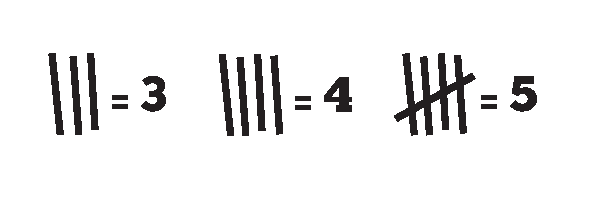
\includegraphics{pictures/Kuva1-1-tukkimiehenkirjanpito.pdf}
\end{center}

Hienostuneempi versio tukkimiehen kirjanpidosta ovat \termi{roomalaiset luvut}{roomalaiset luvut}, jotka nimensä mukaisesti olivat yleisin lukujärjestelmä antiikin Roomassa. Roomalaisia lukuja käytetään yhä nykyäänkin erityisesti järjestyksen merkitsemisessä. Roomalaisten lukujen numeromerkit ovat I, V, X, L, C, D ja M. Ne vastaavat desimaalijärjestelmän lukuja seuraavalla tavalla:

\begin{equation*}
	\textrm{I}=1\quad
	\textrm{V}=5\quad
	\textrm{X}=10\quad
	\textrm{L}=50\quad
	\textrm{C}=100\quad
	\textrm{D}=500\quad
	\textrm{M}=1\,000
\end{equation*}

Roomalaiset luvut merkitään kirjoittamalla merkkejä laskevassa järjestyksessä, poikkeuksena vähennyssääntö. Merkkien kokonaisarvo määrää luvun. Vähennyssääntö tarkoittaa kuutta kaksimerkkistä ilmaisua:

\begin{equation*}
	\textrm{IV}=4\quad
	\textrm{IX}=9\quad
	\textrm{XL}=40\quad
	\textrm{XC}=90\quad
	\textrm{CD}=400\quad
	\textrm{CM}=900
\end{equation*}

Joissain vanhoissa teksteissä (ja jopa kellotauluissa) luku $4$ on merkitty myös IIII.

Luvussa voi olla vain kerran IV tai IX, vain kerran XL tai XC ja vain kerran CD tai CM. Kaksimerkkisiin ilmaisuihin pätevät samat säännöt kuin numeromerkkeihinkin: I$=1$ ei voi edeltää numeroa IV$=4$, eikä IV$=4$ numeroa V$=5$. Lisäksi merkinnät IXV, XCL ja CMD eivät ole sallittuja. Oikea roomalainen luku minimoi käytettyjen merkkien määrän. Esimerkiksi VIV ei ole roomalainen luku, sillä IX on esityksenä lyhyempi.

\termi{nolla}{Nollaa} roomalaisissa numeroissa ei ole; nolla nykyisessä merkityksessään kehitettiin vasta Intiassa 800-luvulla jaa.

\newpage % VIIMEISTELY
\begin{esimerkki}
	Roomalaisia lukuja:
	\alakohdat{
		§ III$=1+1+1=3$
		§ IX$=10-1=9$
		§ XII$=10+1+1=12$
		§ XIV$= 10 + (5 - 1) = 14$
		§ CDX$=500-100+10=410$
		§ MDC$=1\,000+500+100=1\,600$
	}
\end{esimerkki}

\begin{tehtavasivu}

\begin{tehtava}
Muunna seuraavat binääriluvut kymmenjärjestelmään.
	\alakohdat{
		§ $101,0_2$
		§ $1,00101_2$
		§ $100101,1101_2$
	}
\begin{vastaus}
	\alakohdatm{
		§ $5,0_{10}$
		§ $1,15625_{10}$
		§ $37,8125_{10}$
	}
\end{vastaus}
\end{tehtava}

\begin{tehtava}
Muunna seuraavat luvut binäärijärjestelmään.
	\alakohdatm{
		§ $7,0_{10}$
		§ $2,5_{10}$
		§ $11,1875_{10}$
	}
\begin{vastaus}
	\alakohdatm{
		§ $111,0_2$
		§ $10,1_2$
		§ $1011,0011_2$
	}
\end{vastaus}
\end{tehtava}

\begin{tehtava}
Muuta seuraavat kymmenjärjestelmän luvut heksadesimaaliluvuiksi.
\alakohdat{§ $175$ § $384$}
\end{tehtava}

\begin{tehtava}
	Laske
	\alakohdat{
		§ $1101_2 \cdot 100_2$ %joskus tulevaisuudessa meillä on esimerkkejä jakokulmasta binääriluvuille ;_;
		§ $1101001_2 \cdot 100000_2$
		§ $10110_2 \cdot 0,01_2$.
	}
	\begin{vastaus}
		\alakohdat{
			§ $110100_2$
			§ $110100100000_2$
			§ $101,1_2$
		}
	\end{vastaus}
\end{tehtava}

\begin{tehtava}
Mitkä seuraavista ovat oikeita roomalaisia lukuja? Mitä ne ovat kymmenjärjestelmässä?
\alakohdatm{
§ CLI
§ IVX
§ VIZI
§ CCLI
§ CCCLXXXVI
§ CMVCI
§ MMDCXLIIII
§ CDXCIII
§ DCXLIX
} 
\begin{vastaus}
\alakohdatm{
§ $151$
§ Ei ole oikea roomalainen luku.
§ Ei ole oikea roomalainen luku.
§ $251$
§ $386$
§ Ei ole oikea roomalainen luku.
§ Ei ole oikea roomalainen luku.
§ $493$
§ $649$
}
\end{vastaus}
\end{tehtava}

\begin{tehtava}
Muuta seuraavat kymmenjärjestelmän luvut roomalaisiksi luvuiksi. Kuinka monta merkkiä tarvitaan luvun kirjoittamiseen?
\alakohdatm{
§ $278$
§ $712$
§ $1\,478$
§ $3\,999$
}
\begin{vastaus}
\alakohdat{
§ CCLXXVIII, $9$ merkkiä 
§ DCCXII, $6$ merkkiä
§ MCDLXXVIII, $10$ merkkiä
§ MMMCMXCIX, $9$ merkkiä
}
\end{vastaus}
\end{tehtava}

\begin{tehtava}
Tunnetusti $10\cdot 10=100$. Samannäköiseen tuloon päädytään myös, vaikka luku tulkittaisiin kaksikantaisena: $10_2 \cdot 10_2 = 2_{10}\cdot 2_{10}=4_{10}=100_2$. Tutki, päteekö tulo yleisesti, eli onko $10_n\cdot 10_n = 100_n$ myös kaikilla $n >2$.
	\begin{vastaus}
$10_n=1\cdot n^1+0\cdot n^0=n$, eli $10_n \cdot 10_n =n\cdot n = n^2= 1\cdot n^2 + 0 \cdot n^1 + 0\cdot n^0 =100_n$. Väite siis pätee kaikilla kantaluvuilla. (Huomaa, että välivaiheiden eksponentit ja kertoimet ovat kymmenjärjestelmän lukuja.)
	\end{vastaus}
\end{tehtava}

\begin{tehtava}
Muodosta kertotaulu binääriluvuille $1$--$100$.
	\begin{vastaus}
\begin{tabular}{|c||c|c|c|c|}
	\hline 
	$\cdot$ & $1$ & $10$ & $11$ & $100$ \\
	\hline
	\hline
	$1$ & $1$ & $10$ & $11$ & $100$ \\
	\hline 
	$10$ & $10$ & $100$ & $110$ & $1000$  \\
	\hline 
	$11$ & $11$ & $110$ & $1001$ & $1010$ \\
	\hline 
	$100$ & $100$ & $1000$ & $1010$ & $10000$ \\
	\hline 
	\end{tabular} 	
	\end{vastaus}
\end{tehtava}

\begin{tehtava}
	$\star$ Mikä on suuruusjärjestyksessä $148$. positiivinen kokonaisluku, jonka kymmenjärjestelmäesityksessä on vain nollia ja ykkösiä?
	\begin{vastaus}
		$10\,010\,100$
	\end{vastaus}
\end{tehtava}

%\begin{tehtava}
%tallennustilasta, kuinka paljon tilaa tarvitaan tallentaamaan jokin luku halutullal tarkkuudella binäärijärejstelmäääs
%	\begin{vastaus}
%
%	\end{vastaus}
%\end{tehtava}

\end{tehtavasivu}}
    \section*{Paraabeli} \addcontentsline{toc}{section}{Paraabeli} \lukufilter{LIITE_paraabeli}{\subsection*{Toisen asteen polynomin kuvaaja}
\label{paraabeli_tod}

Tässä liitteessä perustellaan, miksi kaikkien toisen asteen polynomifunktioiden kuvaajat näyttävät samalta. Lisäksi tarkastellaan, mitkä tekijät vaikuttavat kuvaajien muotoon.

\underline{Funktio $P(x)=x^2$}

Aloitetaan funktiosta $P(x)=x^2$. Mitä tiedämme siitä piirtämättä kuvaajaa?
\luettelo{
§ Algebrallisen päättelyn avulla voimme todeta, että funktion pienin arvo on $P(0) = 0$, sillä tulon merkkisäännön perusteella lauseke $x^2$ ei voi saada negatiivisia arvoja – ei ole olemassa sellaista reaalilukua $x$, jonka neliö olisi negatiivinen. (Kompleksiluvuilla tällaista rajoitusta ei ole, tästä lisää liitteessä.) Kuvaajan alin kohta sijoittuu siis origoon ja kuvaajan kaikki muut pisteet sen yläpuolelle.
§ Kun $x > 0$, lauseke $x^2$  on sitä
suurempi, mitä suurempi $x$ on. Tästä tiedämme, että nollasta oikealle siirryttäessä funktion kuvaaja nousee.
§ Koska $(-x)^2 = x^2$, kuvaaja on symmetrinen $y$-akselin suhteen.
}

Näiden tietojen avulla voimme päätellä, että funktion kuvaaja koostuu kahdesta
identtisestä haarasta, jotka kohtaavat, kun $x=0$. Mitä kauempana $x$ on nollasta, sitä suurempia ovat funktion arvot. Tämän kaiken voi päätellä jo ennen kuvaajan piirtämistä.

Merkitsemällä koordinaatistoon yhtälön $y=x^2$ toteuttavia pisteitä, muodostuu lopulta funktion kuvaaja:
\begin{center}
\begin{kuvaajapohja}{2}{-2}{2}{-1}{4}
  \kuvaaja{x**2}{$f(x)=x^2$}{blue}
\end{kuvaajapohja}
\end{center}

% FIXME: ongelmallista: ''alaspäin aukeava'' vasta seuraavaksi
Kuvaajan muoto on geometriselta nimeltään \emph{paraabeli}. Paraabeleja esiintyy monessa yhteydessä: esimerksi polttopeilin ja radioteleskoopin pinta kaareutuu paraabelin muotoisena. Samoin ilmaan heitetyn kappaleen rata on likimain alaspäin aukeava paraabeli, kun ilmanvastus on pieni.

\underline{Funktio $P(x)=ax^2, \quad a\neq 0$}

Polynomien $P(x)=ax^2$ arvot ovat ovat lausekkeeseen $x^2$ nähden $a$-kertaisia. Muuten paraabelin symmetrisyys ja muut keskeiset ominaisuudet säilyvät.

\luettelo{
§ Kun $a > 0$, myös $ax^2\geq 0$, joten pienin arvo on yhä $0$.\\
Paraabeli on \termi{ylöspäin aukeava}{ylöspäin aukeava}.
§ Kun $a < 0$, tulon merkkisäännön nojalla $ax^2 \leq 0$. \\
 Nyt $P(0)=0$ onkin suurin arvo, ja funktion arvot ovat sitä pienempiä,
mitä enemmän $x$ poikkeaa nollasta. \\
Paraabeli on \termi{alaspäin aukeava}{alaspäin aukeava}.
§ Mitä enemmän $a$ poikkeaa nollasta, sitä nopeammin funktion arvot
muuttuvat $x$:n muuttuessa ja sitä kapeampi paraabeli on.
}

\begin{center}
$a>0$, paraabeli aukeaa ylöspäin:\\
\begin{tabular}{cc}
$f(x)=\frac{1}{2}x^2$& $f(x)=2x^2$ \\
\begin{kuvaajapohja}{1}{-2}{2}{-1}{4}
  \kuvaaja{0.5*x**2}{}{blue}
\end{kuvaajapohja} &
\begin{kuvaajapohja}{1}{-2}{2}{-1}{4}
  \kuvaaja{2*x**2}{}{blue}
\end{kuvaajapohja}
\end{tabular}

$a<0$, paraabeli aukeaa alaspäin:\\
\begin{tabular}{cc}
$f(x)=-\frac{1}{2}x^2$ & $f(x)=-2x^2$ \\
\begin{kuvaajapohja}{1}{-2}{2}{-4}{1}
  \kuvaaja{-0.5*x**2}{}{blue}
\end{kuvaajapohja} &
\begin{kuvaajapohja}{1}{-2}{2}{-4}{1}
  \kuvaaja{-2*x**2}{}{blue}
\end{kuvaajapohja}
\end{tabular}
\end{center}

\underline{Funktio $P(x)=ax^2+c$}

Lisäämällä vakiotermi $c$ saadaan $P(x)=ax^2+c$. Vakion lisääminen nostaa tai laskee funktion kuvaajaa (riippuen siitä, onko $c > 0$ tai $c<0$), joten kuvaajan muoto ei muutu.

\underline{Funktio $P(x)=ax^2+bx+c$}

Miksi sitten täydellisen toisen asteen polynomin $P(x)=ax^2+bx+c$ kuvaaja on myös paraabeli? Muokataan lauseketta, aloitetaan ottamalla yhteinen tekijä:
\begin{align*}
P(x) &=ax^2+bx+c \\
&= a\left(x^2 +\frac{b}{a}x\right) + c  \quad &
\text{ lavennetaan } \frac{b}{a} \text{ kahdella} \\
&= a\left(x^2 +2\cdot x \cdot \frac{b}{2a} \quad\right) + c  &
\text{ täydennetään neliöksi lisäämällä} \left( \frac{b}{2a} \right)^2 \\
&= a \Bigg( \underbrace{x^2 +2\cdot x \cdot \frac{b}{2a}+\left(\frac{b}{2a} \right)^2}_{\left( x+\frac{b}{2a} \right)^2}
- \left(\frac{b}{2a}\right)^2 \Bigg)  + c \\
&= a \left( \left( x + \frac{b}{2a} \right )^2-\frac{b^2}{4a^2} \right) + c &
\text{ kerrotaan sulut auki } \\
&= a \underbrace{\left(  x + \frac{b}{2a} \right)^2}_{\text{neliö}}-
\underbrace{\frac{b^2}{4a} + c}_{\text{vakio}}
\end{align*}

Tästä neliöksi täydennetyksi muodosta nähdään, että $P(x)$ on muotoa
$a\cdot$neliö + vakio. Kuvaaja on siis samanlainen kuin tapauksessa
$ax^2+c$, huippu on vain siirtynyt.
Koska neliö $\geq 0$, saadaan

\luettelo{
§ Kun $a>0$, kyseinen vakio on polynomin pienin arvo ja kuvaaja on
ylöspäin aukeava paraabeli.
§ Kun $a<0$, kyseinen vakio on suurin arvo ja kuvaaja on alaspäin
aukeava paraabeli.
}

Paraabelin \termi{huippu}{huippu} (eli kuvaajan piste, jossa suurin tai pienin arvo
saavutetaan) on aina kohdassa
$x=-\frac{b}{2a}$, koska silloin neliö on nolla.

%Toisen asteen polynomifunktio on muotoa $f(x)=ax^2+bx+c$, jossa $a,b,c \in \R$ ja $a \neq 0$. Toisen asteen polynomifunktion kuvaaja on paraabeli. Toisen asteen polynomifunktioita käytetään matemaattisessa mallinnuksessa talouden, tieteen ja tekniikan aloilla. Esimerkiksi heittoliikkeessä olevan kappaleen lentorata on aina paraabelin muotoinen. \\
%\textbf{Esimerkki 1.}
%a) Piirrä funktion $f(x)=x^2-2$ kuvaaja. \\
%b) Ratkaise funktion $f$ nollakohdat. \\ \\
%
%\begin{kuvaajapohja}{1}{-2}{2}{-3}{1}
%  \kuvaaja{x**2-2}{$f(x)=x^2-2$}{blue}
%\end{kuvaajapohja}
%
%Funtkion kuvaaja on ylöspäin aukeava paraabeli, joka leikkaa x-akselin kohdissa joissa $f(x)=0$. \\
%Graafisesti funktion nollakohdat saadaan ratkaistua kuvaajasta. Kuvaajasta nähdään, että funktion nollakohdat ovat $x_1 \approx 1,4$ ja $x_2 \approx -1,4$. \\
%Algebrallisesti saadaan ratkaistua, että funktion nollakohdat ovat
%\begin{align*}
%f(x)&=0 \\
%x^2-2&=0 \\
%x^2&=2 \\
%x&= \pm \sqrt[]{2}
%\end{align*}
%Funktion $f$ kuvaajasta huomataan, että se on symmetrinen y-akselin suhteen.
%
%\textbf{Esimerkki 2.} \\
%Piirrä funktioiden $f(x)=x^2+1$, $g(x)=2x^2$ ja $h(x)=\frac{1}{3}x^2$ kuvaajat. \\ \\
%
%\begin{kuvaajapohja}{1}{-2}{2}{-1}{3}
%  \kuvaaja{x**2+1}{$f(x)=x^2+1$}{blue}
%\end{kuvaajapohja}
%
%
%\begin{kuvaajapohja}{1}{-2}{2}{-1}{3}
%  \kuvaaja{2*x**2}{$g(x)=2x^2$}{blue}
%\end{kuvaajapohja}
%
%\begin{kuvaajapohja}{1}{-2}{2}{-1}{3}
%  \kuvaaja{(1 / 3.0)*(x**2)}{$h(x)=\frac{1}{3}x^2$}{blue}
%\end{kuvaajapohja}
%
%Mitä tapahtuu funktion kuvaajan muodolle, kun termin $ax^2$ kerroin $a$ muuttuu? \\ \\
%
%\textbf{Esimerkki 3.} \\
%Piirrä funktioiden $f(x)=-x^2+x$, $g(x)=-x^2+2x+1$ ja $h(x)=-x^2+\frac{1}{2}x-1$ kuvaajat. \\
%\missingfigure \\
%Mitä tapahtuu funktion kuvaajan muodolle, kun termin $bx$ kerroin $b$ muuttuu? \\ \\
%
%\textbf{Esimerkki 4.} \\
%Piirrä funktioiden $f(x)=x^2$, $g(x)=x^2-2$ ja $h(x)=x^2+\frac{3}{2}$ kuvaajat. \\ \\
%Mitä tapahtuu funktion kuvaajan muodolle, kun vakiotermi $c$ muuttuu? \\ \\

Koottuna:

\luettelolaatikko{Toisen asteen polynomifunktion $f(x)=ax^2+bx+c$ kuvaaja}{
§ Ylöspäin aukeava paraabeli, kun $a>0$.
§ Alaspäin aukeava paraabeli, kun $a<0$.
§ Sitä kapeampi, mitä suurempi $|a|$ on.
}

% FIXME: selitys tulisi hoitaa ilman itseisarvoa

%\textbf{Esimerkki 5.} \\
%Ratkaise funktion $f(x)=4x^2-13x+8$ nollakohdat.
%\begin{align*}
%f(x)&=0 \\
%4x^2-13x+8&=0 \\
%x&=\frac{-(-13) \pm \sqrt[]{(-13)^2-4 \cdot 4 \cdot 8}}{2 \cdot 4} \\
%x&=\frac{13 \pm \sqrt[]{169-128}}{8} \\
%x&=\frac{13 \pm \sqrt[]{41}}{8} \\
%x&=\frac{13 \pm \sqrt[]{41}}{8}
%\end{align*}




%Kuvaajaan transformaatioihin esimerkkiä myös muuttujan x muuttamisesta. Piirrä f(x+1):n kuvaaja jne.}
    %\nluku{LIITE_aksioomat}{Reaalilukujen aksioomat}
    %\nluku{LIITE_sanasto}{Hakemisto ja suomi–ruotsi–englanti-sanasto}

\Closesolutionfile{ans}

\osa{Vastaukset ja hakemisto}
\vast
% hakemisto tulee yleisestä rakenteesta
